%*******10********20********30********40********50********60********70********80

% For all chapters, use the newdefined chap{} instead of chapter{}
% This will make the text at the top-left of the page be the same as the chapter

\chap{Θεωρητικό Υπόβαθρο και Σχετική Βιβλιογραφία} \label{c:complex}
%ΠΕΡΙΓΡΑΦΗ ΤΟΥ ΤΙ ΑΚΡΙΒΩΣ ΠΑΡΟΥΣΙΑΖΕΤΑΙ ΣΤΟ ΚΕΦΑΛΑΙΟ

Στο συγκεκριμένο κεφάλαιο γίνεται επεξήγηση των βασικών εννοιών και τεχνολογιών που αναφέρονται στην εργασία. Παρουσιάζονται οι έννοιες της Επαυξημένης Πραγματικότητας, του μοντέλου κάμερας pinhole, της ανίχνευσης δεικτών (markers) και το πεδίο της αναγνώρισης χειρονομιών σε εφαρμογές. Επιπλέον γίνεται ανασκόπηση των σχετικών επιστημονικών εργασιών και εφαρμογών, καθώς και των ανοικτών προκλήσεων στον ερευνητικό τομέα.



\section{Επαυξημένη Πραγματικότητα}
%ΟΡΙΣΜΟΣ+ΤΙ ΥΠΑΡΧΕΙ ΣΗΜΕΡΑ+ΔΙΑΦΟΡΑ ΑΠΟ VR+ OTI EXEI NA KANEI ME AR APO ERGASIES ALLON


%verykokou
Ο όρος επαυξημένη πραγματικότητα, διεθνώς γνωστή ως augmented reality (AR), αναφέρεται στην τεχνολογία που επιτρέπει την προσθήκη ψηφιακών πληροφοριών, που παράγονται από έναν υπολογιστή, στον πραγματικό κόσμο, μέσω κατάλληλων συσκευών. Πρόκειται για ένα ταχέως εξελισσόμενο ερευνητικό πεδίο, το οποίο στοχεύει στον εμπλουτισμό της αντίληψης της πραγματικότητας από το χρήστη.


Ιδανικά, τα αντικείμενα που συμπληρώνουν τον πραγματικό κόσμο παρουσιάζονται να συνυπάρχουν στον ίδιο χώρο με αυτόν. Ωστόσο, δεν αποτελούν μόνο οπτικές πληροφορίες. Η επαυξημένη πραγματικότητα, δυνητικά, μπορεί να βελτιώσει και τις πέντε αισθήσεις, και κυρίως – εκτός από την όραση – την ακοή και την αφή, αν και σήμερα η κυρίαρχη χρήση της είναι η προσθήκη οπτικών πληροφοριών στον πραγματικό κόσμο. 


Υπάρχουν διάφοροι ορισμοί της επαυξημένης πραγματικότητας, εκ των οποίων ευρέως αποδεκτός είναι ο ορισμός που έδωσε ο Ronald Azuma το 1997 \cite{azuma1997}. Σύμφωνα με αυτόν, η επαυξημένη πραγματικότητα είναι μία παραλλαγή της εικονικής πραγματικότητας (virtual reality), αλλά δε θα πρέπει να συγχέεται με την τελευταία, διότι συμπληρώνει τον πραγματικό κόσμο και δεν τον υποκαθιστά. 



Στόχος της εικονικής πραγματικότητας είναι η πλήρης «εμβύθιση» του χρήστη σε ένα περιβάλλον πλήρως ελεγχόμενο από υπολογιστή, το οποίο δεν του επιτρέπει να δει τον πραγματικό κόσμο γύρω του. Οι χρήστες εμβυθίζονται σε μία σκηνή που αν και αποτελείται εξ' ολοκλήρου από γραφικά, γίνται αντιληπτή σαν να ήταν πραγματική.  Για να δημιουργηθεί μια ρεαλιστική εικονική σκηνή, το επίπεδο των λεπτομερειών των γραφικών που συνιστούν τα αντικείμενα της εικονικής σκηνής πρέπει να είναι ιδιαίτερα υψηλό και η απεικόνιση πρέπει να πραγματοποιείται σε πραγματικό χρόνο. Ωστόσο όσο υψηλότερο είναι το επίπεδο των λεπτομερειών, τόσο μειώνεται η απόδοση ενός συστήματος προσπαθώντας να τα απεικονίσει. Ο συνθετικός αυτός κόσμος μπορεί να μιμείται τις ιδιότητες ενός πραγματικού κόσμου, είτε αυτός υπάρχει είτε όχι, ή και να διαφέρει σημαντικά από την πραγματικότητα, δημιουργώντας ένα φανταστικό κόσμο, στον οποίο οι φυσικοί νόμοι δεν ισχύουν πλέον [8]. 


Η επαυξημένη πραγματικότητα στοχεύει στην ενσωμάτωση συνθετικών πληροφοριών στο πραγματικό περιβάλλον – ή σε ένα βίντεο του πραγματικού περιβάλλοντος – με αποτέλεσμα αυτό να μην αποκρύπτεται εντελώς, αλλά αντίθετα να έχει κυρίαρχο ρόλο. Τα εικονικά αντικείμενα σε ένα περιβάλλον επαυξημένης πραγματικότητας, δεν είναι απαραίτητο να έχουν ένα υψηλό επίπεδο λεπτομερειών. Η ρεαλιστική ποιότητά τους περιορίζεται μόνο από τις παραμέτρους της εφαρμογής. 

Μία ακόμα διαφορά ανάμεσα σε συστήματα επαυξημένης και εικονικής πραγματικότητας βασίζεται στο ποσοστό του περιεχομένου της σκηνής που απεικονίζεται. Ένα σύστημα επαυξημένης πραγματικότητας, στο οποίο απεικονίζονται μόνο μερικά απλά εικονικά αντικείμενα σε μία σκηνή, απαιτεί λιγότερη ισχύ από ένα σύστημα εικονικής πραγματικότητας, στο οποίο πρέπει να απεικονίζεται ολόκληρη η σκηνή.


Επιπλέον, διαφορές ανάμεσα στα δύο συστήματα παρατηρούνται στο πρόβλημα του registration(γεωαναφορά). Αφού το registration ασχολείται με τη σωστή τοποθέτηση εικονικών αντικειμένων εντός ενός πραγματικού περιβάλλοντος, τα συστήματα εικονικής πραγματικότητας δεν επηρεάζονται, αφού έχουν να κάνουν μόνο με εικονικές σκηνές. Η θέση όλων των αντικειμένων σε μία σκηνή VR περιγράφεται με βάση ένα κοινό σύστημα συντεταγμένων. Αυτό σημαίνει ότι ένα σύστημα VR έχει πάντα σωστό registration χωρίς να πρέπει να σπαταλά υπολογιστικούς πόρους για την εύρεσή του. Όσον αφορά την απόδοση, το χαμηλό υπολογιστικό κόστος για απεικόνιση γραφικών χαμηλής ποιότητας αντισταθμίζεται από το υπολογιστικό κόστος που απαιτείται για το registration.

Τέλος, στα συστήματα VR, οι συσκευές απεικόνισης χρησιμοποιούνται για να ανιχνεύουν τη τη θέση του χρήστη μαζί με μία οθόνη που απεικονίζει την ψηφιακή σκηνή. Σε ένα σύστημα επαυξημένης πραγματικότητας, υπάρχουν πολλοί διαφορετκοί συνδυασμοί εξοπλισμοί για την ανίχνευση και την πληροφόρηση του χρήστη.
%---

Τα συστήματα επαυξημένης πραγματικότητας σύμφωνα με την καταπληκτική ερευνητική επισκόπηση του πεδίου από τους Azuma et al. (2001) έχουν τα ακόλουθα τρία χαρακτηριστικά \cite{azuma2001}:

\begin{itemize}
\item Συνδυάζουν το πραγματική με την εικονική πληροφορία
\item Επιτρέπουν την αλληλεπίδραση σε πραγματικό χρόνο
\item Λειτουργούν αναφορικά με τον πραγματικό τρισδιάστατο κόσμο
\end{itemize}  


Τα παραπάνω χαρακτηριστικά καθίστανται σημαντικά στην αξιολόγηση αν ένα σύστημα είναι σύστημα επαυξημένης πραγματικότητας ή όχι. Έτσι, για παράδειγμα, κάποιες ταινίες, μολονότι μπορεί να περιλαμβάνουν φωτορεαλιστικά εικονικά αντικείμενα τα οποία συνδυάζονται ομαλά με το τρισδιάστατο πραγματικό περιβάλλον, δεν είναι διαδραστικές σε πραγματικό χρόνο και επομένως δεν αποτελούν συστήματα επαυξημένης πραγματικότητας \cite{azuma1997}. Αντίθετα, η εισαγωγή των εικονικών δεδομένων οφείλεται σε προεπεξεργασία, η οποία αντιτίθεται με το δεύτερο χαρακτηριστικό των συστημάτων επαυξημένης πραγματικότητας.

%augmented virtuality continuum
Σύμφωνα με τους Paul Milgram et al. (1994), η επαυξημένη πραγματικότητα ανήκει στην τεχνολογία της μικτής πραγματικότητας (mixed reality) [8].

Στη δημοσίευσή τους, ορίζεται το «συνεχές πραγματικότητας - εικονικότητας» (reality - virtuality continuum), το οποίο μπορεί να χρησιμοποιηθεί για τη σύγκριση των διαφόρων μορφών της μεικτής πραγματικότητας με την τοποθέτησή τους σε ένα φάσμα, όπως φαίνεται στην Εικόνα 1-1. 

Στη μία άκρη του φάσματους βρίσκεται το πραγματικό περιβάλλον, που δεν περιέχει καμία εικονική πληροφορία. Ενώ μετακινούμαστε προς τα δεξιά, εντοπίζεται η επαυξημένη πραγματικότητα, όπου τα τεχνητά αντικείμενα προστίθενται στον φυσικό κόσμο. Αμέσως πιο δεξιά, εντοπίζεται η επαυξημένη εικονικότητα, όπου τα αντικείμενα του φυσικού κόσμου(όπως μία ζωντανή απεικόνιση μίας απομακρυσμένης προβολής) προστίθενται σε ένα πλήρως εικονικό περιβάλλον "εμβύθισης". Φτάνοντας στο δεξί άκρος του φάσματος, παρατηρείται ένα πλήρως συνθετικό περιβάλλον, στο οποίο δεν υπάρχει καμία πληροφορία από τον φυσικό κόσμο.Κάθε είδος 3D περιβάλλοντος μπορεί να τοποθετηθεί κατά μήκος του φάσματος και μπορεί να χρησιμοποιηθεί για την εύκολη σύγκριση των χαρακτηριστικών του.

Επομένως στο περιβάλλον μεικτής πραγματικότητας, αντικείμενα του πραγματικού και του εικονικού κόσμου – δηλαδή οτιδήποτε μεταξύ των άκρων του συνεχούς – παρουσιάζονται μαζί σε μία συσκευή θέασης. Η μεικτή πραγματικότητα περιλαμβάνει τόσο την επαυξημένη πραγματικότητα, όσο και την επαυξημένη εικονικότητα (augmented virtuality). Ενώ στην πρώτη, το περιβάλλον που παρατηρείται είναι κυρίως αληθινό και έχουν προστεθεί βελτιώσεις που παράγονται από υπολογιστή, στην επαυξημένη εικονικότητα το παρατηρούμενο περιβάλλον είναι κυρίως εικονικό και επαυξάνεται με τη χρήση πραγματικών δεδομένων.

%ADD IMAGE OF CONTINUUM

Αυτός ο ορισμός δεν περιορίζει την επαυξημένη πραγματικότητα στη χρήση μόνο συσκευών απεικόνισης που τοποθετούνται στο κεφάλι του χρήστη(HMDs), επιτρέποντας τη χρήση προβολέων και φορητών συσκευών απεικόνισης, αλλά απκλείοντας μη διαδραστικά μέσα όπως οι ταινίες και τα τηλεοπτικά δρώμενα. 

Για να υπερθέσουμε τρισδιάστατα εικονικά μοντέλα σε αυτ΄που βλέπουν οι χρήστες, ένα σύστημα ΑR πρέπει να συνδυάζει τις πληροφορίες που παράγονται από έναν υπολογιστή με αισθητήρες που μπορούν να μετρήσουν τη θέση και τον προσανατολισμό του χρήστη. 

Καθώς ο χρήστης κινείται στο φυσικό κόσμο, η απεικόνιση των πληροφοριών ανανεώνεται σε πραγματικό χρόνο από τον υπολογιστή. Η ακρίβεια της τοποθέτησης των εικονικών αντικειμένων πάνω στο φυσικό κόσμο επηρεάζει τον ρεαλισμό της εμπειρίας του χρήστη.


%-----------


%AR=Combination of Computer Graphics & COmputer Vision
Ουσιαστικά η επαυξημένη πραγματικότητα αποτελεί συνδυασμό του κλάδου των Γραφικών Υπολογιστών και της Όρασης Υπολογιστών. Ο συνδυασμός αλγορίθμων και μεθόδων των δύο αυτών συγγενών επιστημών είναι το κλειδί για την επίτευξη σημαντικών αποτελεσμάτων σε εφαρμογές που επεξεργάζονται εικόνες ή βίντεο, εξάγουν πληροφορίες από μία σκηνή και επαυξάνουν τη σκηνή με γραφικά.

Για να μπορέσει ο υπολογιστής να δημιουργήσει συναφείς πληροφορίες, πρέπει πρώτα να κατανοήσει κάποιες παραμέτρους. Οι παράμετροι αυτοί έχουν να κάνουν με πληροφορίες σχετικά με το περιβάλλον στο οποίο βρίσκεται ο χρήστης, καθώς και με τη θέση και τον προσανατολισμό του μέσα στο περιβάλλον αυτό. Με βάση αυτές τις πληροφορίες, ο υπολογιστής μπορεί να τοποθετήσει τις επαυξημένες πληροφορίες σωστά σε σχέση με τoν περιβάλλοντα χώρο. Αυτή η εναρμόνιση των εικονικών αντικειμένων με αντικείμενα της πραγματικής σκηνή είναι γνωστή με τον όρο registration. 

Η ανάπτυξη των τεχνικών της όρασης υπολογιστών συντελεί στην καλύτερη αναγνώριση της σκηνής και την εξαγωγή χαρακτηριστικών που βοηθούν στη γνώση της ακριβούς τοποθεσίας στην οποία πρέπει να τοποθετηθούν τα εικονικά αντικείμενα. Ορισμένες ερευνητικές μέθοδοι που αναπτύχθηκαν στο πεδίο της όρασης υπολογιστών εφαρμόζονται και σε συστήματα επαυξημένης πραγματικότητας. Μερικές από αυτές είναι ο εντοπισμός και η ανίχνευση markers και χαρακτηριστικών μία σκηνής, η ανίχνευση και ο εντοπισμός κίνησης, η ανάλυση εικόνας, η αναγνώριση χειρονομιών και η κατασκευή περιβαλλόντων που περιέχουν έναν αριθμό από διαφορετικούς αισθητήρες.


Από την άλλη πλευρά, τα γραφικά συντελούν στην επαύξηση της πραγματικότητας με τη φωτορεαλιστική απεικόνιση τρισδιάστατων μοντέλων σε πραγματικό χρόνο, και τις διαδραστικές κινήσεις τους (animations)

%-------------------------------------------------


Ένα τυπικό σύστημα επαυξημένης πραγματικότητας μπορεί να διαιρεθεί σε 2 κύριες εργασίες: το tracking και το registration.
Πρέπει δηλαδή να ανιχνευθεί ένα γνωστό πρότυπο που είναι αποθηκευμένο στη μνήμη ενός υπολογιστή(marker tracking) \cite{krevelen2010} και έπειτα να προστεθεί ένα εικονικό αντικείμενο στη σκηνή σωστά πάνω σε αυτό το πρότυπο.



\subsection{Ιστορική Αναδρομή}
%ΣΥΝΤΟΜΗ ΙΣΤΟΡΙΚΗ ΑΝΑΔΡΟΜΗ ΑΠΟ ΑΛΛΕΣ ΕΡΓΑΣΙΕΣ

Η τεχνολογίας της επαυξημένης πραγματικότητας υπαινίσσεται για πρώτη φορά το 1901, μέσα από το μυθιστόρημά του Frank Baum με τίτλο «The Master Key», όπου περιγράφεται ένα ζευγάρι ειδικών γυαλιών, το οποίο υπερθέτει στο μέτωπο του κάθε ανθρώπου, που βρίσκεται στο οπτικό πεδίο εκείνου που φοράει τα γυαλιά, ένα γράμμα το οποίο περιγράφει το χαρακτήρα του. [1] [9].


Τα πρώτα πρωτότυπα επαυξημένης πραγματικότητας(Fig. 3), δημιουργήθηκαν από τον πρωτοπόρο στην επιστήμη των γραφικών υπολογιστών Ivan Sutherland και τους φοιτητές του στα πανεπιστήμια του Harvard και της Utah, την δεκαετία του 1960 [151]. Συγκεκριμένα κατασκεύασαν μία τρισδιάστατη συσκευή απεικόνισης που τοποθετείται στο κεφάλι του χρήστη, ενώ παράλληλα κρέμεται από το ταβάνι, με σκοπό να επαυξήσει την σκηνή με τρισδιάστατες πληροφορίες, παρουσιάζοντας στο χρήστη μία προοπτική εικόνα, η οποία αλλάζει καθώς αυτός κουνά το κεφάλι του ή κινείται σε μία περιορισμένη περιοχή. Λόγω των ειδικών κατόπτρων στα πρίσματα μέσω των οποίων ο χρήστης κοιτάζει, μπορεί να βλέπει ταυτόχρονα τόσο τις εικόνες αυτές όσο και αντικείμενα από τον πραγματικό χώρο. Οι εικόνες που παρουσιάζονται στο χρήστη είναι εικόνες διάφανων τρισδιάστατων αντικειμένων, τα οποία αποτελούνται μόνο από τις κύριες ακμές τους και όχι συμπαγών τρισδιάστατων αντικειμένων, λόγω των τεχνικών περιορισμών της εποχής. Το συγκεκριμένο σύστημα θεωρείται, ωστόσο, το πρώτο σύστημα επαυξημένης πραγματικότητας και είναι πραγματικά καινοτόμο για την εποχή. \cite{sutherland1968head}


 

Το 1975 ο Myron Krueger δημιουργεί ένα εργαστήριο τεχνητής πραγματικότητας με το όνομα "Videoplace" στο Πανεπιστήμιο του Κονέκτικατ στις Ηνωμένες Πολιτείες, το οποίο αποτελείται από δύο ή περισσότερα δωμάτια που μπορεί να απέχουν οποιαδήποτε απόσταση μεταξύ τους, μία οθόνη προβολής σε κάθε δωμάτιο και ειδικό hardware, έτσι ώστε οι χρήστες να βλέπουν την εικόνα τους ως μία λευκή σιλουέτα στην οθόνη προβολής να κάνει τις ίδιες κινήσεις με αυτούς. Ταυτόχρονα, δίνεται η δυνατότητα αλληλεπίδρασης με γραφικά αντικείμενα της οθόνης, όπως κείμενο. Επίσης, η εικόνα κάθε χρήστη μπορεί να χρωματιστεί, να σμικρυνθεί ή να περιστραφεί, ενώ γενικά προσφέρονται πολλοί τρόποι αλληλεπίδρασης, όπως η ζωγραφική με τα δάκτυλα [12], [13], [14]. 


Στις αρχές της δεκαετίες του 1990, και συγκεκριμένα το 1992, επινοείται ο όρος "επαυξημένη πραγματικότητα" από δύο επιστήμονες που εργάζονταν στη Boeing, τους Caudell and Mizell [42], οι οποίοι ανέπτυξαν ένα πειραματικό σύστημα επαυξημένης πραγματικότητας για να βοηθήσουν τους εργάτες να συναρμολογήσουν τις πολύπλοκες δέσμες καλωδίων των αεροσκφών[21]. Η εικόνα Figure 1 παρουσιάζει το HMD που αναπτύχθηκε.


Το ίδιο έτος, οι Steven Feiner, Blair MacIntyre και Doree Seligmann παρουσιάζουν το πρώτο κύριο άρθρο πάνω σε ένα πρωτότυπο σύστημα επαυξημένης πραγματικότητας (βλ. Εικόνα 1-4). Tο σύστημα αυτό, με την ονομασία KARMA («Knowledge-based Augmented Reality Maintenance Assistance»), χρησιμοποιεί ένα σύστημα HMD για την υποβοήθηση του τελικού χρήστη κατά τη συντήρηση ενός εκτυπωτή laser \cite{feiner1993knowledge}.



Το 1994, όπως αναφέραμε και σε προηγούμενη ενότητα, ο Paul Milgram παρουσίασε το συνεχές εικονικότητας-πραγματικότητας\cite{milgram1994taxonomy}, το οποίο αποκαλείται και συνεχές επαυξημένης πραγματικότητας. Την ίδια χρονιά, η επαυξημένη πραγματικότητα εισάγεται στο χώρο της τέχνης και της διασκέδασης, αφού δημιουργείται η πρώτη θεατρική παραγωγή επαυξημένης πραγματικότητας με την ονομασία «Dancing in Cyberspace», στην οποία χορευτές και ακροβάτες αλληλεπιδρούν με εικονικά αντικείμενα σε πραγματικό χρόνο, τα οποία προβάλλονται στη σκηνή [1], [17], [20]. 



Το 1995 ο Jun Rekimoto αναπτύσσει το πρώτο φορητό σύστημα χειρός επαυξημένης πραγματικότητας που βασίζεται σε έγχρωμους επίπεδους στόχους, ευρέως γνωστούς μέχρι σήμερα ως markers, το επονομαζόμενο NaviCam (βλ. Εικόνα 1-5). Το 1996 ο ίδιος δημιουργεί ένα 2D barcode σύστημα για εφαρμογές επαυξημένης πραγματικότητας (βλ. Εικόνα 1-6), που βασίζεται σε ασπρόμαυρα τετράγωνα markers δύο διαστάσεων, το CyberCode. Αυτός ο τύπος marker χρησιμοποιείται ακόμα και σήμερα \cite{arth2015history}


Το 1997, ο Ronald Azuma δημοσίευεσε μία αναλυτική έρευνα πάνω στο πεδίο της επαυξημένης πραγματικότητας\cite{azuma1997}, ενώ το 1998 οι Bruce Thomas et al. [25] επιχειρούν να επεκτείνουν την επαυξημένη πραγματικότητα σε εξωτερικούς χώρους, αφού αναπτύσσουν ένα οπτικό σύστημα πλοήγησης για πεζούς, το «Map-in-hat». Πρόκειται για ένα φορητό υπολογιστικό σύστημα, εφοδιασμένο με λογισμικό πλοήγησης, με μία διάφανη συσκευή θέασης, ψηφιακή πυξίδα και GPS (βλ. Εικόνα 1-7). To σύστημα αυτό, ενώ αρχικά περιορίζεται μόνο σε εφαρμογές πλοήγησης, αργότερα εξελίσσεται στο σύστημα Tinmith, που χρησιμοποιείται σε πληθώρα εφαρμογών επαυξημένης πραγματικότητας [21].

Το 1999 ιδρύεται η εταιρία Total Immersion μία από τις πρώτες εταιρίες ανάπτυξης λύσεων επαυξημένης πραγματικότητας, η οποία με το προϊόν της, D’Fusion, παρέχει μία πληθώρα εργαλείων για δημιουργία εφαρμογών επαυξημένης πραγματικότητας [4], [26].

Την ίδια χρονιά, ο Hirokazu Kato αναπτύσσει τη βιβλιοθήκη για εφαρμογές επαυξημένης πραγματικότητας ARToolKit, η οποία παρέχεται στο κοινό ως βιβλιοθήκη ανοικτού κώδικα από το εργαστήριο ΗΙΤ Lab (Human Interface Technology Laboratory) του Πανεπιστημίου της Washington. H βιβλιοθήκη αυτή επιτρέπει τη λήψη βίντεο και την τοποθέτηση – σε πραγματικό χρόνο – εικονικών μοντέλων πάνω σε markers που εντοπίζονται στην εκάστοτε σκηνή, έτσι ώστε να ακολουθούν την κίνηση της κάμερας. Η βιβλιοθήκη ARToolKit αποτελεί τη βάση για πολλές εφαρμογές επαυξημένης πραγματικότητας που ακολουθούν και χρησιμοποιείται ευρέως ακόμα και σήμερα ως έχει ή ελαφρώς παραλλαγμένη.



Έκτοτε σημειώνονται σημαντικά βήματα προόδου στον τομέα της επαυξημένης πραγματικότητας και όλο και περισσότεροι επιστήμονες, αλλά και εταιρίες δείχνουν ενδιαφέρον για την τεχνολογία αυτή, με αποτέλεσμα να αναπτύσσεται πληθώρα εφαρμογών. Από τα επιτεύγματα των ετών αυτών, έως το 2013, κρίνεται σκόπιμη η παράθεση κάποιων σταθμών - σημαντικών γεγονότων στην ιστορία της επαυξημένης πραγματικότητας.

Λόγω της ραγδαίας ανάπτυξης του κλάδου της επαυξημένης πραγματικότητας, ο R.Azuma δημοσίευσε και νέα έρευνα το 2001\cite{azuma2001}, όπου αναλύει τις νεότερες εφαρμογές και καινοτομίες που παρουσίαστηκαν.
Την ίδια χρονιά δημιουργείται το πρώτο πρόγραμμα περιήγησης επαυξημένης πραγματικότητας, Real-World Wide Web (RWWW), από τους Bob Kooper και Blair MacIntyre [30], μια εφαρμογή που υπερθέτει δεδομένα από τον Παγκόσμιο Ιστό (World Wide Web) στον πραγματικό κόσμο, μέσω μίας συσκευής HMD. Τα δεδομένα αυτά ανανεώνονται ανάλογα με τη θέση και τον προσανατολισμό του χρήστη.
Επίσης την ίδια χρονιά, οι Vlahakis et al. παρουσιάζουν το Archeoguide, ένα σύστημα επαυξημένης πραγματικότητας για μνημεία πολιτιστικης κληρονομιας 
το οποίο δημιουργείται για τον ιστορικό χώρο της Αρχαίας Ολυμπίας στην Ελλάδα. Περιλαμβάνει μία διεπαφή πλοήγησης στο χώρο, τρισδιάστατα μοντέλα αρχαίων ναών και αγαλμάτων, καθώς και εικονικούς δρομείς που συναγωνίζονται για τη νίκη στο αρχαίο στάδιο.


Το 2002, ο Mann [25] προσέθεσε έναν ακόμα άξονα στο συνεχές πραγματικότητας-εικονικότητας του Milgram για να καλύψει και άλλες μορφές του φάσματος. Το νέο αυτό δισδιάστατο συνεχές που παρουσίασε, ορίζει τις έννοιες mediated reality και mediated virtuality (see left illustration in Figure 3). Όπως αναφέρεται, ένα σύστημα μπορεί να αλλάξει την πραγματικότητα με διάφορους τρόπους. Μπορεί να προθέσει κάτι (augmented reality), να αφαιρέσει κάτι (diminished reality), ή να μετατρέχει κάτι σε κάτι άλλο (modulated reality). Με τον όρο diminished reality, αναφερόμαστε στη διαδικασία κατά την οποία αφαιρούμε από τη περιβάλλον πραγματικά αντικείμενα της σκηνής. Επομένως η diminished reality είναι κατά κάποιον τρόπο το αντίθετο της επαξημένης πραγματικότητας. 

Επίσης, την ίδια χρονιά (2002) διοργανώνεται το πρώτο διεθνές συνέδριο μικτής και επαυξημένης πραγματικότητας, International Symposium on Mixed Reality and Augmented Reality (ISMAR), το οποίο διοργανώνεται σε ετήσια βάση μέχρι και σήμερα και δίνει τη δυνατότητα στους ερευνητές να ανταλλάσσουν ιδέες, σκέψεις και συμπεράσματα \cite{ismar}.


Το 2006 η Nokia εισάγει το πρόγραμμα MARA (Mobile Augmented Reality Applications project). H πρωτότυπη αυτή εφαρμογή χρησιμοποιεί εργαλεία όπως επιταχυνσιόμετρο, πυξίδα και GPS για τον υπολογισμό της θέσης και του προσανατολισμού του κινητού τηλεφώνου, με αποτέλεσματην υπέρθεση πληροφοριών για πραγματικά αντικείμενα σε ζωντανό βίντεο, εκμεταλλευόμενη τις δυνατότητες του κινητού τηλεφώνου [36], [37], ενώ το 2008 δημιουργείται το πρόγραμμα περιήγησης επαυξημένης πραγματικότητας Wikitude από την Αυστριακή εταιρία Mobilizy GmbH (βλ. Εικόνα 1-10), μία εφαρμογή επαυξημένης πραγματικότητας βάσει θέσης, που αξιοποιεί τα χαρακτηριστικά και την κάμερα ενός κινητού τηλεφώνου για να υπερθέσει πληροφορίες από το διαδίκτυο για τον περιβάλλοντα χώρο σε βίντεο, σε πραγματικό χρόνο.[39].

Το 2009, η εταιρία SPRXmobile δημιουργεί το πρόγραμμα περιήγησης επαυξημένης πραγματικότητας Layar, μία παραλλαγή του Wikitude [21]. Με την εφαρμογή αυτή, ανιχνεύοντας με το κινητό τηλέφωνο το περιεχόμενο διαφόρων προϊόντων, όπως εφημερίδες και περιοδικά που συνοδεύονται από το σήμα του Layar, οι χρήστες μπορούν να δουν επιπρόσθετο ψηφιακό υλικό, όπως για παράδειγμα βίντεο σχετικό με τη στατική εικόνα που απεικονίζεται. Επίσης, παρέχεται και η δυνατότητα σε όποιον θέλει – επί πληρωμή – να προσθέσει ψηφιακό υλικό σε στατικές εικόνες, με το προϊόν Layar Creator.

Το 2010 η Microsoft δημιούργησε τη συσκευή Kinect η οποία αποτέλεσε τη βάση για την ανάπτυξη εφαρμογών επαυξημένης πραγματικότητας και κυρίως βιντεοπαιχνιδιών σε μεγαλύτερη κλίμακα.

Το 2012 η εταιρεία Oculus VR ανακοινώνει τη συσκευή ανάπτυξης Oculus Rift, ένα HMD εικονικής πραγματικότητας head-mounted display. Η δημοσιότητα που έλαβε η δημιουργία του συγκεκριμένου προϊόντος αποτέλεσε την αρχή για τη δημιουργία μιας σειρά από head-mounted displays κυρίως για το χώρο της βιομηχανίας των βιντεοπαιχνιδιών. (see Fig.17(a)).


To 2013 διατίθεται το Google Glass μέσω του προγράμματος "Explorer", το οποίο είχε ανακοινωθεί ως Project Glass το 2012 από την Google και συγκεντρώνει θετικά και αρνητικά σχόλια, καθώς και προβληματισμό σχετικά με την προστασία των προσωπικών δεδομένων(see Fig.17(b). Ωστόσο η διάθεση του συγκεκριμένου προϊόντος σταμάτησε το 2015.

Τον Ιανουάριο του 2015, η Microsoft ανακοίνωσε τη συσκευή Hololens,η οποία συνδυάζει την εικονική και την επαυξημένη πραγματικότητα [93]. Πρόκειται για μία συσκευή η οποία είναι ένας ολοκληρωμένος υπολογιστής με μία see-through display και αρκετούς αισθητήρες.\cite{hololens}
Το 2015 μία από τις μεγαλύτερες εταιρίες ανάπτυξης εργαλείων λογισμικού επαυξημένης πραγματικότητας, η Metaio, η οποία δημιούργησε το Junaio, έναν περιηγητή επαυξημένης πραγματικότητας για φορητές συσκευές Android και iOS, εξαγοράστηκε από την Apple σε μία κίνηση\cite{applemetaio} που δείχνει πως το μέλλον της ανθρωπότητας θα είναι σίγουρα "επαυξημένο". 


Η επαυξημένη πραγματικότητα είναι μία τεχνολογία που μπορεί να αξιοποιηθεί από πολλούς επιστημονικούς κλάδους και επιτρέπει την ανάπτυξη πληθώρας εφαρμογών. Σήμερα γίνονται προσπάθειες για την αξιοποίηση των δυνατοτήτων της πολλά υποσχόμενης εν λόγω τεχνολογίας σε διάφορους τομείς, μέσω της ανάπτυξης εφαρμογών που απευθύνονται σε άτομα με διαφορετικά ενδιαφέροντα και ασχολίες.




\subsection{Εφαρμογές} \label{sec:apps}
%ΑΝΑΦΕΡΕ ΧΑΡΑΚΤΗΡΙΣΤΙΚΕΣ ΕΦΑΡΜΟΓΕΣ ΣΕ GAMING,IATRIΚΗ, MILITARY,TOURISM

Στην ενότητα αυτή καταγράφονται οι κυριότεροι τομείς στους οποίους η επαυξημένη πραγματικότητα έχει εφαρμογή και αναφέρονται συνοπτικά διάφορα αντιπροσωπευτικά είδη εφαρμογών σε κάθε τομέα. 

Η τεχνολογίας της Επαυξημένης Πραγματικότητας μπορεί να αξιοποιηθεί σε πολλές περιοχές εφαρμογών. Αυτές περιλαμβάνουν  It is well suited for on-site visualisation both indoors and outdoors, for visual guidance in assembly, maintenance and training.

Η επαυξημένη πραγματικότητα επιτρέπει τη δημιουργία διαδραστικών βιντεοπαιχνιδιών και εναλλακτικών τρόπων διαφήμισης προϊόντων. Επίσης μπορεί να χρησιμοποιηθεί για τη σύνδεση τρισδιάστατων γραφικών και βίντεο με έντυπα όπως περιοδικά ή διαφημιστικά φυλλάδια. Τέλος, έχει δοκιμαστεί σε ιατρικές εφαρμογές για διάφορους σκοπούς. Στη συνέχεια παρουσιάζονται χρήσεις της επαυξημένης πραγματικότητας και παραδείγματα εφαρμογών, που δείχνουν πώς αξιοποιήθηκε.  



%AR for entertainment and gaming

Η επαυξημένη πραγματικότητα έχει διεισδύσει στον τομέα της ψυχαγωγίας, δείχνοντας τις συναρπαστικές δυνατότητές της. Κυκλοφορούν πολλά παιχνίδια επαυξημένης πραγματικότητας, τα οποία προσελκύουν το κοινό λόγω της δυνατότητας που του προσφέρουν να αλληλεπιδρά σε πραγματικό χρόνο τόσο με πραγματικά όσο και με εικονικά αντικείμενα. Μπορεί να απευθύνονται σε έναν ή περισσότερους χρήστες και να χρησιμοποιούν κινητά τηλέφωνα, υπολογιστές, φορητούς ή μη, ή ΗΜDs, προσφέροντας μοναδικές εμπειρίες στους χρήστες. Πέρα όμως από τα παιχνίδια, υπάρχουν και λογοτεχνικά βιβλία επαυξημένης πραγματικότητας για παιδιά αλλά και κόμικς [47], όπου τρισδιάστατες σκηνές της ιστορίας παρουσιάζονται πάνω από τις πραγματικές σελίδες και καθιστούν πιο ενδιαφέρουσα την εμπειρία του διαβάσματος. Κοινή είναι πλέον η χρήση της στα καθημερινά δελτία καιρού. Ο τηλεθεατής. μέσω του δέκτη του, βλέπει τον παρουσιαστή μπροστά από το χάρτη πρόγνωσης του καιρού, ο οποίος στην πραγματικότητα δεν υπάρχει. Με χρήση της επαυξημένης πραγματικότητας, το φόντο μπροστά από το οποίο βρίσκεται ο παρουσιαστής, αντικαθίσταται σε πραγματικό χρόνο από το χάρτη, ο οποίος μάλιστα περιλαμβάνει κινούμενα γραφικά στοιχεία. Η επαυξημένη πραγματικότητα χρησιμοποιείται και στον αθλητισμό και η τεχνολογία αυτή εφαρμόζεται ήδη κατά την αναμετάδοση αγώνων. Ένα παράδειγμα αποτελεί η παραγόμενη από υπολογιστή κίτρινη γραμμή που φαίνεται στα γήπεδα των ποδοσφαιρικών αγώνων στους τηλεοπτικούς δέκτες (βλ. Εικόνα 1-15) και είναι ορατή μόνο από τους τηλεθεατές, διευκολύνοντάς τους στην κατανόηση τυχούσας παράβασης των κανονισμών του παιχνιδιού [1], [48]. Επίσης, η επαυξημένη πραγματικότητα χρησιμοποιείται σε πληθώρα αθλητικών γεγονότων για να δείξει διαφημίσεις να υπερτίθενται σε συγκεκριμένες περιοχές της μεταδιδόμενης εικόνας [1], [7].


%krevelen
Όπως η εικονική πραγματικότητα, έτσι και η επαυξημένη πραγματικότητα μπορεί να εφαρμοστεί στη βιομηχανία της ψυχαγωγίας για τη δημιουργία παιχνιδιών, αλλά και για την ενίσχυση  σημαντικών γεγονότων που λαμβάνουν χώρα κατά τη μετάδοση αγώνων και αθλημάτων. 
Οι πισίνες, οι αγωνιστικοίς χώροι, οι πίστες αγώνων ταχύτητας και άλλα παρόμοια περιβάλλοντα έχουν γνωστές ιδιότητες και χαρακτηριστικά, με αποτέλεσμα η επαύξηση του βίντεο το οποίο τα απεικονίζει να μπορεί να γίνει εύκολα. Ένα παράδειγμα είναι το σύστημα Fox-Trax [43], που χρησιμοποιείται για την επισήμανση της τοποθεσίας μιας σφαίρας hockey, η οποία δεν φαίνεται εύκολα, καθώς μετακινείται γρήγορα στον πάγο. Επίσης η επαυξημένη πραγματικότητα μπορεί να χρησιμοποιηθεί για την ζωντανή απεικόνιση της απόδοσης κολυμβητών αλλά και για την ζωντανή κατάταξη οδηγών σε αγώνες ταχύτητας.  Χάρη στα προβλεπόμενα περιβάλλοντα(ομοιόμορφοι παίκτες σε πράσινα, λευκά ή μπλε πίστες), οι επισημάνσεις απεικονίζονται στην πίστα αλλά όχι πάνω στους παίκτες.(Fig. 21b).



Το 2000 οι Bruce Thomas et al. [29] δημιουργούν το πρώτο παιχνίδι επαυξημένης πραγματικότητας, το ARQuake, που αποτελεί μία παραλλαγή του διάσημου παιχνιδιού Quake για ηλεκτρονικό υπολογιστή (βλ. Εικόνα 1-8). Το παιχνίδι βασίζεται σε ένα σύστημα ανίχνευσης 6 βαθμών ελευθερίας και χρησιμοποιεί GPS, μία ψηφιακή πυξίδα και οπτική ανίχνευση των επίπεδων στόχων. Οι χρήστες εφοδιάζονται με ένα φορητό υπολογιστή στην πλάτη τους, ένα HMD και μία απλή συσκευή εισόδου [4], [21].

Ένας αριθμός από βιντεοπαιχνίδια για προετοιμασμένα εσωτερικά περιβάλλοντα έχουν αναπτυχθεί, όπως το παιχνίδι μάχης ενάντια σε εξωγήινους "Aqua-
Gauntlet" [155], το "ContactWater", το "ARHockey" και το "2001 AR Odyssey" [154]. Έχουν είσης αναπτυχθεί βιντεοπαιχνίδια επαυξημένης πραγματικότητας όπως το"AR-Bowling" του Matysczok et al. [104] , και το AR tennis για κινητά της Nokia από τους Henrysson et al. [71] created  (Fig. 22).



Τρία είναι εκείνα τα χαρακτηριστικά της επαυξημένης πραγματικότητας που επιτρέπουν την υποστήριξη καινοτόμων βιντεοπαιχνιδιών για υπολογιστές σε σύγκριση με την εικονική πραγματικότητα \cite{Thomas2012}.

\begin{itemize}
\item \textbf{Η Επαυξημένη πραγματικότητα απαιτεί την απεικόνιση γραφικών μόνο σε ένα συγκεκριμένο ποσοστό του οπτικού πεδίου του χρήστη.} Το μεγαλύτερο ποστοστό της σκηνής που βλέπει ο χρήστης αποτελείται από τον πραγματικό κόσμο και μονο τα ψηφιακά αντικείμενα του παιχνιδιού απαιτούν γραφικά που παράγονται από υπολογιστές. Αντίθετα στην εικονική πραγματικότητα, ολόκληρος ο ψηφιακός κόσμος πρέπει να δημιουργηθεί από τους υπολογιστές, προκαλώντας τους χρήστες να νομίζουν ότι βρίσκονται σε έναν συνθετικό κόσμο. Η χρήση βοηθημάτων και συστημάτων απεικόνισης CAVE επιτρέπει πιο φυσική αλληλεπίδραση, αλλά και πάλι ο χρήστης βρίσκεται εγκλωβισμένος σε έναν συνθετικό κόσμο, αν και αυτό δεν είναι πάντα κακό, αφού για παράδειγμα ο χρήστης μπορεί να "μεταφερθεί" σε έναν νέο ψηφιακό κόσμο που δεν υπάρχει στην πραγματικότητα.
  
\item \textbf{Η ιδιότητα της επαυξημένης πραγματικότητας να επιτρέπει στους χρήστες να βλέπουν τον φυσικό κόσμο, παρέχει μία καλύτερη αίσθηση του που βρίσκονται και ποιος είναι γύρω τους.} H δυνατότητα να βλέπουν οι χρήστες τον πραγματικό κόσμο κατά τη διάρκεια του βιντεοπαιχνιδιού επιτρέπει την ελευθερία των κινήσεων και την αποφυγή εμποδίων όπως καρέκλες, δέντρα ή άλλα άτομα. Επίσης το γεγονός ότι μπορούν να βλέπουν άλλα άτομα είναι ένας ιδιαίτερα ενδιαφέρων συνδυασμός για συνεργασία μέσα σε βιντεοπαιχνίδια. Για παράδειγμα, το να στοχεύει ένας χρήστης ένα άλλο άτομο με ένα πραγματικό όπλο ακτίνων laser και να το πυροβολά εικονικά είναι πιο άμεσο από το να πυροβολά έναν εικονικό χαρακτήρα. 
  
\item \textbf{Η φυσικότητα της κίνησης σε ανοιχτούς χώρους είναι πιο ελκυστική για τους χρήστες.} Η κίνηση των χρηστών σε μεγάλες ή μικρές περιοχές επιτρέπει την κατανόηση και την εμπειρία του παιχνιδιού καλύτερα. Το να περπατάει κάποιος σε μία θέση είναι διασθητικά πιο εύκολο από το να χρησιμοποιεί ένα πληκτρολόγιο ή ένα ποντίκι. Επίσης το να μπορεί να σηκώσει πραγματικά αντικείμενα και να τα χρησιμοποιήσει ως συσκευές εισόδου είναι ιδιαίτερα ευχάριστο για το χρήστη.
\end{itemize}

  


%Medical apps

Πέρα από τον τομέα της ψυγαγωγίας, ένα από τα πιο σημαντικά πεδία εφαρμογών της επαυξημένης πραγματικότητας είναι εκείνο του τομέα της ιατρικής, όπου  μπορεί να χρησιμοποιηθεί για τη βοήθεια στη διάγνωση και τη θεραπεία μίας νόσου ή για την εκτέλεση μίας χειρουργικής επέμβασης. 

Για παράδειγμα, τα δεδομένα που συλλέγονται από μία εξέταση όπως είναι η μαγνητική τομογραφία, η αξονική τομογραφία ή οι απεικονίσεις υπερήχων μπορούν να συνδυαστούν έτσι ώστε να υπερτεθούν συγκεκριμένες πληροφορίες σχετικά με την ανατομία ενός ασθενή, πάνω του. Έτσι ο γιατρός έχει τη δυνατότητα να δει στο "εσωτερικό" του ασθενούς κατά την ώρα της εξέτασης και να συμβάλλει στην ολοκλήρωση της διάγνωσης με ένα τρόπο περισσότερο καινοτόμο σε σχέση με μία απλή εξέταση (βλ. Εικόνα 1-11) [1], [4], [42], [43]. Ακόμη, τέτοιου είδους πληροφορίες είναι πολύ σημαντικές στον τομέα της ελάχιστα επεμβατικής χειρουργικής, διότι παρέχουν μία εικόνα του εσωτερικού του ασθενούς, χωρίς την ανάγκη για μεγαλύτερες τομές \cite{fuchs1998augmented}. Κατά τη διάρκεια μίας επέμβασης, η επαυξημένη πραγματικότητα θα μπορούσε να χρησιμοποιηθεί για την αναγνώριση και επισήμανση οργάνων του ασθενούς και μελών του σώματός του στα οποία θα πρέπει – ή θα απαγορεύεται – να επέμβουν οι γιατροί. Παράλληλα, εικονικές οδηγίες θα μπορούσαν να υπενθυμίζουν στο χειρούργο τα βήματα μίας εγχείρισης.

Ο Fuchs et al. [62] παρουσίασε ένα σύστημα για λαπαροσκοπική εγχείριση όπου προσομοιώνεται η θέση των λαπαροσκοπίων που πραγματοποιείται μέσω μικρών τομών στον ασθενή. (Fig. 19). Οι Kotranza and Lok [92] παρατήρησαν ότι η χρήση επαυξημένων ανδρείκελων ασθενών σε συνδυασμό με απτικής ανάδραση είχε ως αποτέλεσμα την επίκληση της ίδιας συμπεριφορά από τους ειδικούς σαν να είχαν μπροστά τους πραγματικούς ασθενείς. 


%GRAPSE GIA TO ARACHNOFOBIA TREATMENT APO HIT LAB NZ




%combat and simulation
Τέλος, πρέπει να σημειωθεί ότι από τη δεκαετία του 70 και μέχρι σήμερα, στρατιωτικές υπηρεσίες σε συνεργασία με διάφορα πανεπιστημιακά ιδρύματα και ερευνητικά κέντρα ασχολούνται με την αξιοποίηση των δυνατοτήτων της επαυξημένης πραγματικότητας, για εφαρμογές σχετικές με τις ανάγκες των σωμάτων στρατού, ναυτικού και αεροπορίας, σε θέματα διεξαγωγής πολεμικών επιχειρήσεων, εκπαίδευσης προσωπικού κ.ά. Μάλιστα αξίζει να αναφερθεί, ότι το μεγαλύτερο μέρος της έρευνας σε πανεπιστήμια και εταιρίες είναι αποτέλεσμα χρηματοδότησης για στρατιωτική έρευνα.


Εφαρμογές επαυξημένης πραγματικότητας αναπτύχθηκαν για τα μαχητικά αεροσκάφη έτσι ώστε να παρέχουν οπτικές ενδείξεις στους πιλότους, επαυξάνοντας τη σκηνή που παρατηρούν.Συγκεκριμένα τα Head-Up Displays (HUDs) αποτελούν μία διάφανη συσκευή που τοποθετείται στο οπτικό πεδίο των πιλότων και δείχνει τις επιπρόσθετες πληροφορίες, επιτρέποντάς τους να έχουν «το κεφάλι ψηλά», ενώ τα Helmet-Mounted Displays (HMDs) προσαρμόζονται στο κράνος τους και προβάλλουν πληροφορίες μπροστά στα μάτια τους. Σε περίπτωση μάχης, ένα σύστημα επαυξημένης πραγματικότητας θα μπορούσε να προβάλλει χρήσιμα δεδομένα σε ειδικά γυαλιά των στρατιωτών σε πραγματικό χρόνο. Για παράδειγμα, άνθρωποι ή διάφορα αντικείμενα θα μπορούσαν να επισημαίνονται με κατάλληλα σήματα, τα οποία να δείχνουν αν πρόκειται για πιθανούς εχθρούς ή κινδύνους. 


Προφανώς οι δυνατότητες ανάπτυξης εφαρμογών επαυξημένης πραγματικότητας εντοπίζονται σε πολλά ακόμα επιστημονικά πεδία, όπως αυτό του τουρισμού, της συναρμολόγησης, των κατασκευών και της διαφήμισης.



\subsection{Περιβάλλον και Τεχνολογίες Επαύξησης}
%ziegler
Ένα από τα σημαντικότερα ζητήματα κατά το σχεδιασμό μιας εφαρμογής επαυξημένης πραγματικότητας είναι πώς θα επιτευχθεί ο συνδυασμός εικονικού και πραγματικού κόσμου. Αυτό επιτυγχάνεται κυρίως μέσω της χρήσης συσκεύων απεικόνισης που προσαρτώνται στο κεφάλι του χρήστη, ωστόσο μπορούν να χρησιμοποιηθούν και φορητές συσκευές.
Μάλιστα οι περισσότερες πειραματικές εργασίες χρησιμοποιούν την οθόνη ενός υπολογιστή, ενός tablet ή ενός κινητού, διότι το κόστος συσκευών HMDs είναι πολύ μεγάλο. 

%--
Ένα απλό σύστημα επαυξημένης πραγματικότητας αποτελείται από μία κάμερα, μία υπολογιστική μονάδα(φορητός υπολογιστής, tablet, etc), μία οθόνη, κατάλληλο λογισμικό και – ανάλογα με την εφαρμογή – διάφορους αισθητήρες (GPS, πυξίδα, επιταχυνσιόμετρα), markers ή εικόνες - πρότυπα προς αναγνώριση και πιθανώς και άλλα.
Η κάμερα καταγράφει την εικόνα μιας πραγματικής σκηνής και έπειτα το σύστημα επαυξάνει την εικόνα προσθέτοντας εικονικά αντικείμενα. Το τελικό αποτέλεσμα εμφανίζεται στην οθόνη.
Η εικόνα \ref{fig:ar_example} παρουσιάζει ένα παράδειγμα απλού συστήματος επαυξημένης πραγματικότητας που βασίζεται στην ανίχνευση ενός ασπρόμαυρου δείκτη (marker).
Πιο συγκεκριμένα το σύστημα καταγράφει τη σκηνή, ανιχνεύει το marker και εξάγει την τοποθεσία και τον προσανατολισμό της κάμερας. Στη συνέχεια επαυξάνει το βίντεο, τοποθετώντας το εικονικό αντικείμενο πάνω στη σκηνή και συγκεκριμένα πάνω στο marker και έπειτα το τελικό επαυξημένο βίντεο παρουσιάζεται στην οθόνη.


\begin{figure}[H]
    \centering
    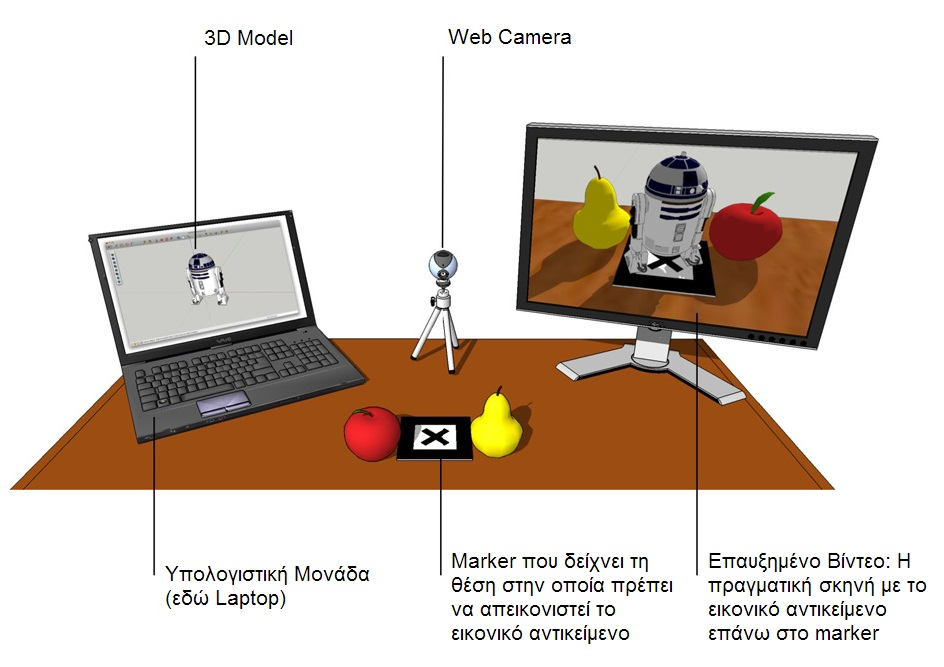
\includegraphics[scale=0.25, angle=0]{Files/Figures/ar_system_example.jpg}
    \caption[Παράδειγμα εγκατάστασης ενός συστήματος επαυξημένης πραγματικότητας ]{ Παράδειγμα εγκατάστασης ενός συστήματος επαυξημένης πραγματικότητας \cite{ar_example}}
    \label{fig:ar_example}
\end{figure}


Η κύρια διαδικασία για τη σωστή λειτουργία ενός συστήματος επαυξημένης πραγματκότητας έχει να κάνει με το κομμάτι της ανίχνευσης. Το κομμάτι αυτό ασχολείται με τον υπολογισμό της σχετικής πόζας της κάμερας σε πραγματικό χρόνο. Με τον όρο πόζα (pose) περιγράφουμε τους 6 βαθμούς ελευθερίας της τοποθεσίας ενός αντικειμένου, δηλαδή τη θέση του στον τρισδιάστατο χώρο και τον προσανατολισμό στον τριασδιάστατο χώρο.

Η διαδικασία της ανίχνευσης είναι αυτή που επιτρέπει την προσθήκη εικονικών αντικειμένων σε μία πραγματική σκηνή.
Η βασική διαφορά σε σύγκριση με άλλα εργαλεία επεξεργασίας εικόνας παρατηρείται στο γεγονός ότι στην επαυξημένη πραγματικότητα τα εικονικά αντικείμενα μετακινούνται και περιστρέφονται σε 3 διαστάσεις αντί για 2 όπως γίνεται συνήθως σε εικόνες.  Ο απλούστερος τρόπος εκτίμησης της πόζας είναι η χρήση δεικτών (markers). 
Ωστόσο, το μαθηματικό μοντέλο ( προβολική γεωμετρία) πίσω από τις μεθόδους υπολογισμού της πόζας είναι το ίδιο. 

Παρόμοια προβλήματα βελτιστοποίησης διαμορφώνονται σε διαφορετικές μεθόδους υπολογισμού της πόζας και λύνονται με τις ίδιες μεθόδους βελτιστοποίησης.  
Μπορούμε να θεωρήσουμε ότι οι markers είναι ένας ειδικός τύπος χαρακτηριστικού και επομένως μπορούμε να ορίσουμε μεθόδους με βάση την ανίχνευση markers και μετέπειτα μεθόδους με βάση την ανίχνευση χαρακτηριστικών, καθώς και υβριδικές μεθόδους. Στη συγκεκριμένη διπλωματική εργασία θα επικεντρωθούμε σε συστήματα επαυξημένης πραγματικότητας που βασίζονται σε markers.

Συνήθως η καταγραφή της εικόνας δεν είναι σημαντικό κομμάτι στην επαυξημένη πραγματικότητα. Συνήθως χρησιμοποιούνται έτοιμες βιβλιοθήκες για το σκοπό αυτό,

Τα εργαλεία και οι βιβλιοθήκες επαυξημένης πραγματικότητας παρέχουν υποστήριξη για την καταγραφή εικόνας και βίντεο. Η διαδικασία τηςα απεικόνισης ζωγραφίζει την εικονική εικόνα πάνω στην εικόνα του βίντεο. Στα γραφικά υπολογιστών, η εικονική σκηνή προβάλλεται πάνω στο επίπεδο της εικόνας χρησιμοποιώντας μία εικονική κάμερα και αυτή η προβολή απεικονίζεται στο τέλος. 

Απαιτείται ουσιαστικά η χρήση μίας εικονικής κάμερας που είναι παρόμοια με τη πραγματική κάμερα του συστήματος. Με αυτό τον τρόπο τα εικονικά αντικείμενα προβάλλονται στη σκηνή με τον ίδιο τρόπο με τον οποίο θα προβάλλονταν πραγματικά αντικείμενα και το αποτέλεσμα είναι γεωμετρικά πειστικό. Για να μπορέσουμε να μιμηθούμε τις ιδιότητες της πραγματικής κάμερας, το σύστημα πρέπει να ξέρει τα οπτικά χαρακτηριστικά της κάμερας. Η διαδικασία κατά την οποία προσδιορίζονται αυτά τα χαρακτηριστικά ονομάζεται βαθμονόμηση κάμερας.

Η βαθμονόμηση της κάμερας μπορεί να είναι μέρος του συστήματος επαυξημένης πραγματικότητας ή ξεχωριστή διαδικασία. Πολλές βιβλιοθήκες παρέχουν εργαλεία βαθμονόμησης, όπως για παράδειγμα οι βιβλιοθήκες ArUco, ALVAR, ARToolkit.


Ωστόσο για τη διαδικασία της βαθμονόμησης μπορούν να χρησιμοποιηθούν και τρίτα εργαλεία βιβλιοθηκών όπως το Matlab ή η OpenCV. 

Στην εργασία αυτή αφού περιγράψουμε τη διαδικασία της βαθμονόμησης, θεωρούμε ότ έχουμε πάντα μία σωστά βαθμονομημένη κάμερα για την ανάπτυξη της εφαρμογής μας.

Η ποικιλία των συσκευών οι οποίες υποστηρίζουν συστήματα επαυξημένης πραγματικότητας είναι μεγάλη και περιλαμβάνει σταθερούς και φορητούς υπολογιστές, tablets, κινητά και άλλες υπολογιστικές μονάδες. Ανάλογα με την εφαρμογή, μπορεί να αξιοποιηθεί η ενσωματωμένη κάμερα της συσκευής, μία απλή USC κάμερα, μία Firewire κάμερα ή μία ψηφιακή κάμερα. Μπορεί επίσης να χρησιμοποιηθεί μία συσκευή απεικόνισης που προσαρτάται στο κεφάλι του χρήστη(HMD), μία συσκευή απεικόνισης οπτικής τεχνολογίας ή η ίδια η οθόνη της υπολογιστικής μονάδας. Επίσης μπορεί το σύστημα να προβάλλει την επαυξημένη σκηνή στον πραγματικό κόσμο\cite{jones2013illumiroom} ή να χρησιμοποιηθεί μια στερεοσκοπική συσκευή απεικόνισης. Η κατάλληλη εγκατάσταση εξαρτάται από την εφαρμογή και το περιβάλλον στο οποίο αναπτύσσεται.









Ο συνδυασμός πραγματικών και εικονικών εικόνων σε μία συγχωνευμένη εικόνα παρουσιάζει τεχνικές δυσκολίες για τους σχεδιαστές εφαρμογών επαυξημένης πραγματικότητας.  Το ερώτημα, στο οποίο καλούνται να απαντήσουν, έχει να κάνει με το πώς θα πραγματοποιηθεί η συνένωση των δύο εικόνων. Στην ενότητα αυτή παρουσιάζονται τα είδη τεχνολογιών θέασης της επαυξημένης σκηνής \cite{azuma1997} \cite{Vallino1998}  \cite{azuma2001}.





-Head-Worn Displays (HWDs)
Οι συσκευές αυτές, γνωστές ως Head-Worn Displays (HWD) ή Head-Attached Displays, φοριούνται στο κεφάλι του χρήστη ή σε κάποιο μέρος του κεφαλιού. Στις παρακάτω παραγράφους περιγράφονται οι κυριότερες κατηγορίες των συσκευών αυτών.\cite{barfield2001fundamentals}


Στην επαυξημένη πραγματικότητα υπάρχουν δύο βασικές κατηγορίες συστημάτων απεικόνισης που αξιοποιούν τα HMDs ως μέσο για την οπτική διεπαφή. 

Επιτυγχάνεται τοποθετώντας οπτικούς μπροστά από τα μάτια του χρήστη. Κάθε σύστημα έχει συγκεκριμένα πλεονεκτήματα και μειονεκτήματα, που σχετίζονται με το σχεδιασμό μιας εφαρμογής και είναι απαραίτητο  να θεωρήσουμε όλες τις παραμέτρους πριν την υλοποίηση του συστήματος AR.Αξίζει να σημειωθεί ότι τα non-immersive HMDs μπορεί να είναι μονοσκοπικά ή στερεοσκοπικά. Οι διαφορές ανάμεσα τους πρέπει να εξεταστούν όταν γίνεται η επιλογή του σχεδιασμού με βάση ένα optical based system. Οι οπτικές προσεγγίσεις είναι απλούστερες και φθηνότερες. Ο κόσμος φαίνεται μέσα από οπτικούς combiners,οπότε υπάρχει μόνο ένα video stream να ανησυχούμε. Στα see-through systems η μόνη διαθέσιμη πληροφορία είναι η θέση της κεφαλής του χρήστη που προέρχεται από έναν head tracker. 



Για την ενίσχυση της "εμβύθισης" του χρήστη χρειάζονται διάφορες τεχνολογίες απεικόνισης της επαυξημένης σκηνής. Τα HMDs έχουν ευρεία χρήση σε εφαρμογές εικονικής πραγματικότητας. Ένα σύστημα Head-Mounted Display (HMD) είναι μία συσκευή που προσαρτάται στο κεφάλι του χρήστη και συνδυάζει την εικόνα του πραγματικού κόσμου με εικονικά αντικείμενα, μέσω χρήσης οπτικής ή βίντεο τεχνολογίας. 
Στο πεδίο της επαυξημένης πραγματικότητας χρησιμοποιούνται 2 είδη HMD. Συγκεκριμένα τα video see-through and optical see-through. Ο όρος “see-through” προέρχεται από την ανάγκη του χρήστη να μπορεί να βλέπει τον πραγματικό κόσμο που βρίσκεται μπροστά του, ακόμα και όταν φοράει το HMD.

 
\textbf{Optical See-Through Displays}


Η τεχνολογία αυτή βασίζεται στη δημιουργία ενός συστήματος παρουσίασης το οποίο προσαρτάται στο κεφάλι του χρήστη (optical see-through HMDs) που απαιτεί την τοποθέτηση "οπτικών συνδυαστών" (συνήθως ημιδιαπερατών και ημιανακλαστικών κάτοπτρων ) μπροστά από τα μάτια του χρήστη, που του επιτρέπουν να δει τόσο το πραγματικό περιβάλλον γύρω του, όσο και τα εικονικά αντικείμενα που παράγονται από τον υπολογιστή. 
Τα εικονικά αντικείμενα ανακλούνται μέσω των κατόπτρων από τις οθόνες που είναι προσαρτημένες στο κεφάλι του, με βάση την τρέχουσα θέση του, όπως φαίνεται στην εικόνα ~\ref{fig:videoseethrough} ).  Επομένως, όταν οι χρήστες μετακινούν τα κεφάλια τους, τα εικονικά αντικείμενα διατηρούν τη θέση τους στον κόσμο σαν να ήταν κομμάτι του πραγματικου περιβάλλοντος.



Τα optical see-through συστήματα δε χρησιμοποιούν καθόλου την είσοδο του σήματος βίντεο, με αποτέλεσμα ο χρήστη να βλέπει το πραγματικό περιβάλλον, και όχι μία αναπαράσταση μέσω βίντεο, πετυχαίνοντας την αξιοποίηση της υψηλής ανάλυσης του πραγματικού κόσμου όπως τον παρατηρεί ο χρήστης. Ουσιαστικά, η συγχώνευση του πραγματικού κόσμου με την εικονική επαύξηση γίνεται οπτικά μπροστά από το χρήστη \cite{Vallino1998} . Αυτή η τεχνολογία είναι παρόμοια με τα  heads up displays (HUD) που χρησιμοποιούνται στα cockpits μαχητικών αεροσκαφών και παρουσιάστηκαν στην προηγούμενη ενότητα~\ref{sec:apps}

Επιπλέον παρουσιάζουν ορισμένα πλεονεκτήματα. Αρχικά θεωρούνται ασφαλή διότι οι χρήστες μπορούν να δουν τη πραγματική σκηνή που βρίσκεται μπροστά τους, ακόμα και αν υπάρξει σφάλμα στην παροχή ισχύος, με αποτέλεσμα η συγκεκριμένη τεχνολογία να είναι ιδανική για στρατιωτικούς και ιατρικούς σκοπούς. Ωστόσο, κι άλλες συσκευές εισόδου όπως κάμερες είναι απαραίτητες για αλληλεπίδραση και registration. Επιπλέον παρουσιάζουν χαμηλό κόστος, και δεν επηρεάζονται από το πρόβλημα της παράλλαξης το οποίο δημιουργεί μία διαφορά ως προς τη θέση των ματιών και της κάμερας \cite{krevelen2010} .


Εφόσον οι χρήστες βλέπουν την πραγματική σκηνή, το εικονικό μέρος είναι ο μόνος λόγος που προκαλείται καθυστέρηση(lag). Για τον ίδιο λόγο, η ποιότητα της σκηνής της προβολής του κόσμου είναι πολύ καλύτερη από την αναπαράσταση μέσω βίντεο. Επομένως η χρήση ενός see-through system εξαλείφει το πρόβλημα της καθυστέρησης του συστήματος και βελτιώνει την ποιότητα προβολής της επαυξημένης σκηνής. 


Ωστόσο πέρα από πλεονεκτήματα, ο συνδυασμός εικονικών αντικειμένων ολογραφικά μέσα από κάτοπτρα και φακούς δημιουργεί και μειονεκτήματα, καθώς μειώνεται η φωτεινότητα, αλλά και η αίσθηση "εμβύθισης" του χρήστη. Επομένως η συγκεκριμένη τεχνική φαίνεται ακατάλληλη για εξωτερική χρήση. Παράλληλα, μία σημαντική παράμετρος, αυτή του πεδίου όρασης του χρήστη (field-of-view) περιορίζεται και μπορεί να προκληθεί ψαλιδισμός των εικονικών εικόνων στα άκρα των ανακλαστήρων. Τέλος, η απόκρυψη των πραγματικών αντικειμένων (occlusion) είναι δυσκολότερη επειδή το φως συνδυάζεται πάντα με την εικονική εικόνα. 

Επιπλέον το γεγονός ότι δεν υπάρχει σήμα βίντεο, αφού δεν υπάρχει κάμερα. Επομένως οι αισθητήρες θέσης μέσα στο HMD είναι ο μόνος τρόπος να εξάγουμε πληροφορίες της πόζας για λόγους registration. Αυτό έχει σαν συνέπεια τη μείωση της ακρίβειας του registration, αν η επιλεγμένη μέθοδος head tracking που χρησιμοποιείται δεν είναι απόλυτα ακριβής \cite{Malik2002} .

H ποιότητα της εικονικής επαύξησης είναι συνήθως χαμηλή, αφού ο μικρός οπτικός συνδυαστής μπροστά από το μάτι του χρήστη είναι χαμηλής ανάλυσης. Έτσι περιορίζεται η εμφάνιση την εμφάνιση των λεπτομερειών των γραφικών που προβάλλονται στην έξοδο. Η ποιότητα των εικονικών αντικειμένων περιορίζεται από την ταχύτητα επεξεργασίας και τις γραφικές ικανότητες του συστήματος επαύξησης. Επομένως η δημιουργία πειστικών επαυξήσεων γίνεται δυσκολότερη αφού ο πραγματικός κόσμος θα εμφανίζεται κανονικά, σε αντίθεση με τα εικονικά αντικείμενα που θα εμφανίζονται pixilated. Αν ένα σύστημα επαυξημένης πραγματικότητας απαιτεί εικονικά αντικείμενα με γραφικά υψηλής ανάλυσης, τότε προτιμώνται συνήθως συστήματα video see-through ή monitor-based \cite{Mcdonald2003} . 


\begin{figure}[H]
    \centering
    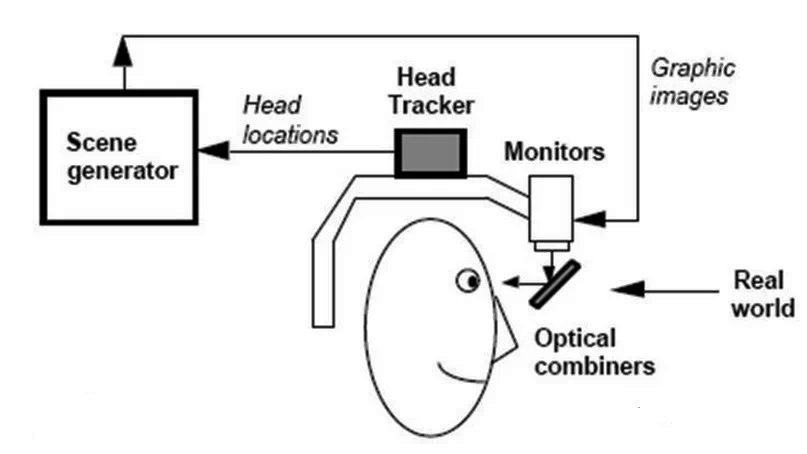
\includegraphics[scale=0.7, angle=0]{Files/Figures/optical.jpg}
    \caption[Διάγραμμα συστήματος Optical See-Through Display \cite{azuma1997}]{ Διάγραμμα συστήματος Optical See-Through Display \cite{azuma1997}}
    \label{fig:opticalseethrough}
\end{figure}



\textbf{Video See-Through Displays}

Τα HMDs που χρησιμοποιούν βίντεο τεχνολογία (video see-through HMDs), συνδυάζουν ένα «κλειστό» HMD (closed-view HMD) και μία ή δύο βιντεοκάμερες προσαρτημένες στο κεφάλι του χρήστη, όπως φαίνεται στην εικόνα ~\ref{fig:videoseethrough} . Η σκηνή του πραγματικού κόσμου καταγράφεται από τις βιντεοκάμερες, οι οποίες του παρέχουν τη δυνατότητα να βλέπει τον πραγματικό κόσμο. Με αυτό τον τρόπο, ο χρήστης δε βλέπει τον πραγματικό κόσμο απευθείας, αλλά αντίθετα βλέπει μόνο αυτό που απεικονίζεται στις μικρές οθόνες στο εσωτερικό του HMD.  

 

Το πλεονέκτημα των συστημάτων τέτοιου τύπου παρατηρείται στο ότι κατά τη καταγραφή της πραγματικής σκηνής μέσω βίντεο, μπορούν να εξαχθούν πληροφορίες για τη σκηνή. Οι ψηφιοποιημένες εικόνες επιτρέπουν την ανίχνευση της κίνησης του κεφαλιού του χρήστη παρέχοντας μεγαλύτερη ακρίβεια κατά τη διαδικασία του tracking της θέσης του κεφαλιού και επομένως οδηγεί σε πιο ακριβές registration. Επιπλέον η απεικόνιση του βίντεο είναι συνήθως υψηλής ανάλυσης και δίνεται η δυνατότητα να απεικονιστούν τα εικονικά αντικείμενα με λεπτομερή γραφικά σε συνδυασμό με το βίντεο εισόδου.Συνεπώς, αυξάνεται η ρεαλιστικότητα και η εμβύθιση του χρήστη που μπορεί να προσφέρει ο επαυξημένος κόσμος \cite{krevelen2010} .


Αυτή η διαδικασία συγχώνευσης προσθέτει ωστόσο καθυστερήσεις στο σύστημα. Οι καθυστερήσεις του συστήματος λόγω της καταγραφής, της επεξεργασίας, της επαύξησης και της απεικόνισης σε κάθε frame του βίντεο μεταφράζεται σε lag που καταλαβαίνει ο χρήστης με αποτέλεσμα να χάνεται η αίσθηση της εμβύθισης. Αυτό είναι ένα μειονέκτημα στα συστήματα video see-through technology που δεν μπορεί να αποφευχθεί αλλά μπορεί να ελαχιστοποιηθεί. Μειονεκτήματα εντοπίζονται επίσης στη χαμηλή ανάλυση απεικόνισης του πραγματικού κόσμου, στο περιορισμένο field-of-view (αν και μπορεί να αυξηθεί εύκολα), και τον αποπροσανατολισμό των χρηστών λόγω της παράλλαξης (eye-offset) λόγω της θέσης της κάμερας σε μία απόσταση από τη πραγματική θέση των ματιών του χρήστη. Τέλος, μία μεγάλη διαφορά ανάμεσα στις κάμερες και τα μάτια του χρήστη, μπορεί να ελλατώσει την αίσθηση της εμβύθισης, αφού τα πάντα στις σκηνές που καταγράφονται θα μετατοπιστούν ψηλότερα ή χαμηλότερα από εκεί που θα έπρεπε να είναι(ως προς την κανονικό επίπεδο της θέσης των ματιών) \cite{Malik2002} . 



\begin{figure}[H]
    \centering
    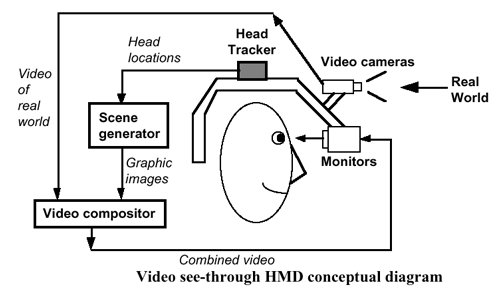
\includegraphics[scale=0.8, angle=0]{Files/Figures/videoseethrough.jpg}
    \caption[Διάγραμμα συστήματος Video See-Through Display \cite{azuma1997}]{ Διάγραμμα συστήματος Video See-Through Display \cite{azuma1997}}
    \label{fig:videoseethrough}
\end{figure}


\textbf{Monitor-based Systems}


Πέρα όμως από τις συσκευές τεχνολογίας HMD, υπάρχουν και συσκεύες απεικόνισης σε οθόνη με χρήση βίντεο-τεχνολογίας. Οι συσκευές αυτές απεικονίζουν τις επαυξημένες σκηνές σε μία κοινή οθόνη, κάνοντας χρήση της επεξεργασίας εικόνας και της μίξης του εικονικού με το πραγματικό. Η απλούστερη προσέγγιση ενός monitor-based συστήματος απεικόνισης, φαίνεται στο~\ref{fig:monitor} .

Το είδος αυτό της επαυξημένης πραγματικότητας αποτελεί μία από τις πιο απλές και αποδοτικές λύσεις, καθώς απαιτεί έναν τυπικό ηλεκτρονικό υπολογιστή και  και μία βιντεοκάμερα USB ή Firewire. Ωστόσο αυτή η απλότητα προκαλεί συνέπειες στον τομέα της εμβύθισης του χρήστη σε περιβάλλοντα επαυξημένης πραγματικότητας, λόγω του σχετικά μικρού μεγέθους της οθόνης και του συνακόλουθου μικρού οπτικού πεδίου. Το σύστημα επαύξησης μπορεί να χρησιμοποιήσει τεχνικές με βάση την όραση υπολογιστών για να υπολογίσει τις πληροφορίες της πόζας(θέση και προσανατολισμός) του χρήστη για σκοπούς registration (ανιχνεύοντας χαρακτηριστικά ή πρότυπα για παράδειγμα).

Ακόμη, μειονέκτημα αποτελεί η ποιότητα της εικόνας, καθώς αυτή περιορίζεται από την ανάλυση της κάμερας. Προφανώς, το να βλέπει κάποιος τον πραγματικό κόσμο μέσα από τη μικρή οθόνη ενός υπολογιστή περιορίζει το ρεαλισμό και την φορητότητα του επαυξημένου κόσμου. Επιπλέον, εφόσο κάθε frame της κάμερας χρειάζεται επεξεργασία από το σύστημα επαύξησης, μπορεί να καταγραφεί καθυστέρηση λόγω του χρόνου από τη στιγμή που καταγράφεται η πραγματική σκηνή, μέχρι να απεικονιστεί η τελική επαυξημένη εικόνα. 




\begin{figure}[H]
    \centering
    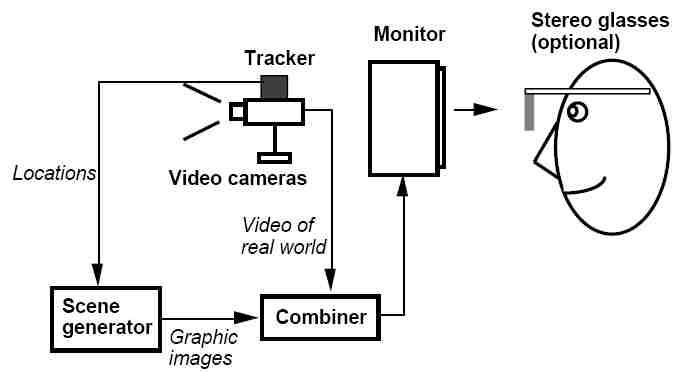
\includegraphics[scale=0.8, angle=0]{Files/Figures/monitor.jpg}
    \caption[Διάγραμμα συστήματος Monitor Display \cite{azuma1997}]{ Διάγραμμα συστήματος Monitor Display \cite{azuma1997}}
    \label{fig:monitor}
\end{figure}


\begin{figure}[H]
    \centering
    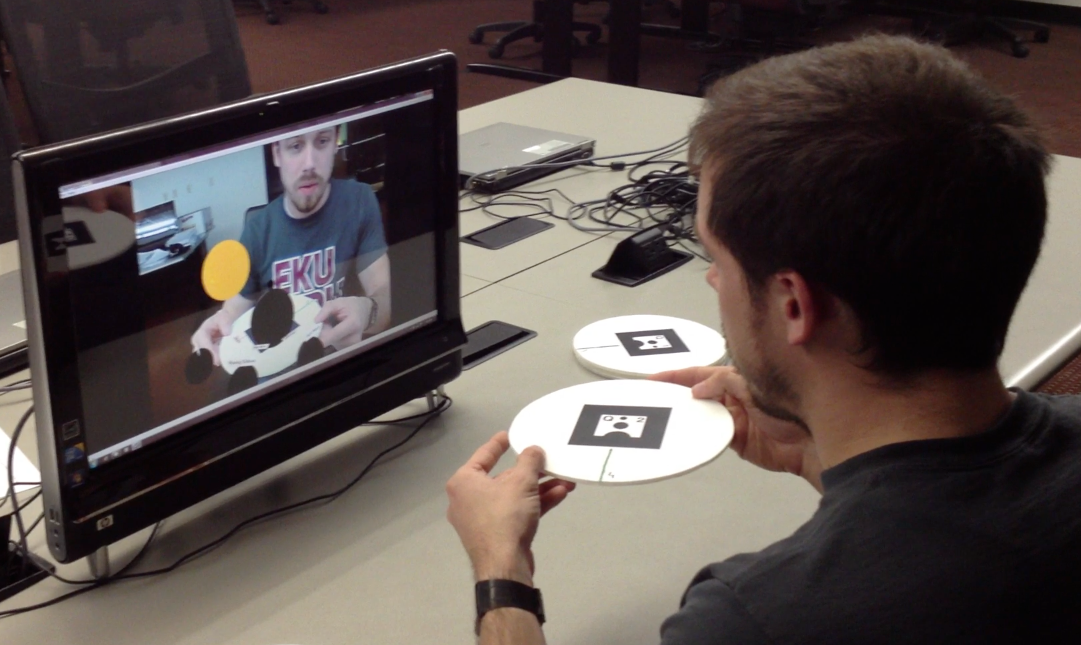
\includegraphics[scale=0.2, angle=0]{Files/Figures/monitor_example.png}
    \caption[Παράδειγμα εφαρμογής μέσω συσκευής απεικόνισης σε
οθόνη \cite{monitor_ar} .]{ Παράδειγμα εφαρμογής μέσω συσκευής απεικόνισης σε
οθόνη \cite{monitor_ar} .}
    \label{fig:monitor_example}
\end{figure}


\textbf{Φορητές Συσκευές}


Οι συσκευές αυτές, ευρέως γνωστές ως Handheld Displays (HDs), περιλαμβάνουν μία οθόνη, μέσω της οποίας είναι δυνατή η θέαση της επαυξημένης σκηνής, και είναι φορητές, μικρού μεγέθους, έτσι ώστε ο χρήστης να μπορεί να τις κρατήσει στο χέρι του και να τις μεταφέρει μαζί του. 

Τέτοιες συσκευές είναι τα κινητά τηλέφωνα – και συγκεκριμένα τα «έξυπνα» κινητά τηλέφωνα, γνωστά ως smartphones – τα tablet PCs και οι – λιγότερο χρησιμοποιούμενοι πλέον – προσωπικοί ψηφιακοί οδηγοί PDAs (Personal Digital Assistants). 

Στη μεγάλη πλειονότητα των εφαρμογών επαυξημένης πραγματικότητας που προορίζονται για φορητές συσκευές χειρός, η βιντεοκάμερα «αιχμαλωτίζει» τη ζωντανή εικόνα του πραγματικού περιβάλλοντος, η οποία επαυξάνεται με επιπρόσθετες γραφικές πληροφορίες πριν την απεικόνισή της στην οθόνη. 

Μέσω των συσκευών αυτών, ο χρήστης δεν «βυθίζεται» στο επαυξημένο περιβάλλον, αλλά το παρακολουθεί μέσω της οθόνης της συσκευής του, γεγονός το οποίο θα μπορούσε να θεωρηθεί ως μειονέκτημα. 

Επίσης, η συνήθως χαμηλή επεξεργαστική ισχύ και μνήμη τους, μπορεί να προκαλέσει καθυστερήσεις κατά την εκτέλεση της εφαρμογής. Ωστόσο οι συσκευές αυτές παρουσιάζουν το πλεονέκτημα του μικρότερου μεγέθους και βάρους \cite{wagner2007handheld} \cite{arth2015history} .

Τα τελευταία χρόνια έχουν αναπτυχθεί και σύγχρονα συστήματα απεικόνισης όπως ειδικοί φακοί επαφής, ωστόσο δε θα αναφέρουμε περισσότερα για τη συγκεκριμένη τεχνολογία.





\section{Marker-based Tracking}
%MONO FIDUCIAL MARKER TRACKING

%eisagogi enotitas
While some approaches seek natural features such as key points or textures,fiducial markers are still an attractive approach because they are easy to detect and high speed, as well as precision may be achieved.


Σε αυτό το κεφάλαιο γίνεται μία εισαγωγή στις μαθηματικές έννοιες της επαυξημένης πραγματικότητας, στις μεθόδους που χρησιμοποιούνται και στην αναγνώριση δεικτών.  
In this chapter, we review prior work in the field of augmented reality from which our research draws upon. We start by providing an introduction to the mathematical concepts of augmented reality, and describe how they relate to the registration problem. We then present a brief survey of various proposed solutions to the registration problem in the current augmented reality literature. We conclude by briefly describing some open issues.

%siltanen
Η επαυξημένη πραγματικότητα παρουσιάζει πληροφορίες στα πλαίσια του πραγματικού κόσμου. Για να συμβεί αυτό, το σύστημα πρέπει να γνωρίζει που βρίσκεται ο χρήστης και προς τα που κοιτά σε κάθε χρονική στιγμή. Συνήθως ο χρήστης εξερευνεί το περιβάλλον μέσα από μία οθόνη που απεικονίζει την εικόνα που καταγράφει η κάμερα μαζί με την επαυξημένη πληροφορία.  
Επομένως, το σύστημα χρειάζεται πρακτικά να ξέρει τη θέση και τον προσανατολισμό της κάμερας, έτσι ώστε να απεικονίσει τα εικονικά αντικείμενα στη σωστή θέση. Αυτή η διαδικασία ονομάζεται tracking και αναφέρεται στον υπολογισμό της σχετικής πόζας(pose) της κάμερας (θέση και προσανατολισμός) σε πραγματικό χρόνο και είναι ένα από τα βασικότερα μέρη ανάπτυξης εφαρμογών επαυξημένης πραγματικότητας.


Οι ερευνητές στα πεδία της όρασης υπολογιστών έχουν αναπτύξει έναν αξιοσημείωτο αριθμό μεθόδων tracking. Οι μέθοδοι αυτές μπορούν να ταξινομηθούν με βάση τον εξοπλισμό που χρησιμοποιείται σε μεθόδους sensor tracking, visual tracking και υβριδικές. Εφόσον στα περισσότερα συστήματα επαυξημένης πραγματικότητας χρησιμοποιείται συνήθως μία κάμερα, οι τεχνικές visual tracking είναι αυτές που παρουσιάζουν μεγαλύτερο ενδιαφέρον, οπότε θα επικεντρωθούμε σε αυτές.


Στα συστήματα visual tracking, η πόζα της κάμερας μπορεί να υπολογιστεί με βάση την παρατήρηση των σκηνών που καταγράφει. Σε ένα άγνωστο περιβάλλον, παρατηρούνται πολλές δυσκολίες, καθώς απαιτείται αρκετός χρόνος προκειμένου να γίνει η συλλογή αρκετών δεδομένων για τον υπολογισμό της πόζας και επιπλέον, η εκτίμηση των υπολογισμών ολισθαίνει με την πάροδο του χρόνου. Καθώς το περιβάλλον δεν είναι γνωστό στο σύστημα, ο προσανατολισμός του άξονα συντεταγμένων επιλέγεται τυχαία, κάτι το οποίο μπορεί να μην είναι ιδιαίτερα βολικό για το χρήστη. Επιπλέον, είναι αδύνατο να υπολογιστεί η σωστή κλίμακα μόνο με βάση τις οπτικές παρατηρήσεις. Μία λύση που θα μπορούσε να ξεπεράσει αυτές τις δυσκολίες, εντοπίζεται στην εισαγωγή ενός ανιχνεύσιμου προκαθορισμένου στόχου στο περιβάλλον και στη χρήση τεχνικών όρασης υπολογιστών για τον εντοπισμό του στη σκηνή. 

Ο στόχος αυτός είναι ουσιαστικά ένας δείκτης ή marker, ένα σημάδι ή μια εικόνα, που μπορεί να εντοπιστεί από ένα υπολογιστικό σύστημα μέσω του βίντεο χρησιμοποιώντας τεχνικές επεξεργασίας εικόνας, αναγνώρισης προτύπων και υπολογιστικής όρασης (π.χ~\ref{fig:marker})). Μόλις εντοπιστεί ένας marker, μπορεί να οριστεί η σωστή θέση και ο προσανατολισμός της κάμερας. Αυτή η προσέγγιση ονομάζεται ανίχνευση βασισμένη σε marker (marker-based tracking) και χρησιμοποιείται ευρύτατα στην επαυξημένη πραγματικότητα.%vale link

\begin{figure}[H]
    \centering
    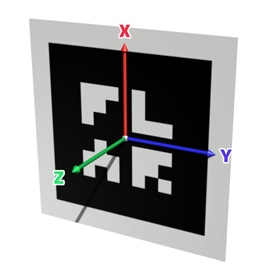
\includegraphics[scale=0.6, angle=0]{Files/Figures/marker-axis.jpg}
    \caption[Παράδειγμα marker]{ Παράδειγμα marker}
    \label{fig:marker}
\end{figure}




Άλλες προσεγγίσεις χρησιμοποιούν ανίχνευση με βάση τον εντοπισμό οπτικών χαρακτηριστικών και εντοπισμό προκαθορισμένων μοντέλων. Στον εντοπισμό με βάση προκαθορισμένα μοντέλα, το σύστημα γνωρίζει εκ των προτέρων τις ιδιότητες ενός μοντέλου ή μέρους της σκηνής (π.χ CAD μοντέλο). Πραγματοποιείται σύγκριση ανάμεσα στα frames που κταγράφονται και γίνεται προσπάθεια να γίνει αντιστοίχηση του μοντέλου με ένα μέρος της σκηνής. Μόλις συμβεί αυτό, μπορεί να υπολογιστεί και η πόζα της κάμερας. Στη διαδικασία feature-based tracking,το σύστημα προσπαθεί να ανιχνεύσει οπτικά χαρακτηριστικά της σκηνής μέσα από τις εικόνες και να γνωρίσει το περιβάλλον με βάση ορισμένες παρατηρήσεις κινήσεων ανάμεσα σε διαδοχικά frames. Αν και η επικρατούσα τάση στην έρευνα σχετικά με το visual tracking τείνει προς το feature-based tracking, που δεν απαιτεί την εκτύπωση και χρήση markers, οι μέθοδοι που βασίζονται σε markers παρουσιάζουν καλύτερες επιδόσεις από τις μεθόδους feature-based σε συγκεκριμένες περιπτώσεις και χρησιμοποιούνται ακόμα πολύ συχνά σε εφαρμογές επαυξημένης πραγματικότητας \cite{wagner2008robust} \cite{rabbi2014applications} .


Η ευρεία χρήση συστημάτων που λειτουργούν με βάση την ανίχνευση markers εξηγείται και από το γεγονός ότι είναι εύκολα στην υλοποίηση και υπάρχουν πολλά διαθέσιμα εργαλεία για την ανάπτυξη τέτοιων εφαρμογών (π.χ ARToolKit \cite{artoolkit}, ALVAR \cite{alvar}, ArUco \cite{aruco}). Τα εργαλεία αυτά αποτελούν μία καλή βάση για να ξεκινήσει κάποιος την ανάπτυξη εφαρμογών επαυξημένης πραγματικότητας. Επιπλέον, οι markers παρέχουν εκτιμήσεις για τη σωστή κλίμακα και βολικές συντεταγμένες για κάθε frame όπως αναφέρθηκε και προηγουμένως. Μπορούν να κωδικοποιήσουν πληροφορίες ή να έχουν απλά ένα ID. Κάτι τέτοιο, επιτρέπει στο σύστημα να επισυνάψει συγκεκριμένα αντικείμενα ή αλληλεπιδράσεις στα markers. Στη συστήματα που χρησιμοποιούν marker-based tracking, απαιτείται η ανίχνευση του marker, η ταυτοποίηση του και ο υπολογισμός της πόζας. 

Στις παρακάτω ενότητες, παρουσιάζεται η διαδικασία υπολογισμού της πόζας ενός δείκτη. Αρχικά παρουσιάζονται περιληπτικά οι βασικές αρχές της προβολικής γεωμετρίας και το μοντέλο κάμερας pinhole. Ύστερα αναλύεται η διαδικασία βαθμονόμησης κάμερας με αποτέλεσμα τον υπολογισμό των παραμέτρων της και ο τρόπος ανίχνευσης ενός marker. Στο τέλος της ενότητας παρουσιάζεται ένας τρόπος αξιοποίησης πολλαπλών markers με στόχο τη βελτίωση της επίδοσης του συστήματος.





Στη συνέχεια του κεφαλαίου θα χρησιμοποιήσουμε ομογενείς συντεταγμένες. Οι ομογενείς συντεταγμένες (homogeneous coordinates) είναι ένα είδος συντεταγμένων που χρησιμοποιείται στην προβολική γεωμετρία, αντίστοιχα με τις καρτεσιανές συντεταγμένες που χρησιμοποιούνται στην ευκλείδεια γεωμετρία. Στα πλεονεκτήματά τους συγκαταλέγονται η δυνατότητα αναπαράστασης όλων των σημείων, ακόμα και των σημείων του απείρου, με πεπερασμένες συντεταγμένες, καθώς και η δυνατότητα έκφρασης ενός προβολικού μετασχηματισμού με τη βοήθεια ενός μόνο πίνακα.

Πιο συγκεκριμένα, έστω ένα σημείο της εικόνας με καρτεσιανές συντεταγμένες \[\begin{bmatrix} x \\ y \end{bmatrix}\]
Το αντίστοιχο σημείο, σε ομογενείς συντεταγμένες μπορεί να αναπαρασταθεί ως: \[\begin{bmatrix} wx \\ wy \\ w\end{bmatrix}=
\begin{bmatrix}x'\\y'\\w\end{bmatrix} , w\neq0 \].

Ομοίως στον 3D χώρο ένα σημείο με καρτεσιανές συντεταγμένες \[\begin{bmatrix} x \\ y \\ z \end{bmatrix}\] μπορεί να αναπαρασταθεί ως: \[\begin{bmatrix} wx \\ wy \\ wz \\ w\end{bmatrix}=
\begin{bmatrix}x'\\y'\\z' \\ w\end{bmatrix} , όπου w\neq0 \].


Παρά το γεγονός ότι μπορεί να χρησιμοποιηθεί ένας οποιοσδήποτε μη μηδενικός αριθμός $w$, συνήθως παίρνουμε $w=1$, ώστε η αλλαγή συστήματος συντεταγμένων να γίνεται ευκολότερα.

Ο παρακάτω πίνακας συνοψίζει την αναπαράσταση των σημείων που θα χρησιμοποιηθεί:




\begin{tabu} to 0.9\textwidth { | X[l] | X[c,m] | X[c,m] | }
   \hline
    & Ευκλείδεια Γεωμετρία & Προβολική Γεωμετρία \\[0.5cm]
   \hline
   Σημείο στο 2Δ Χώρο  & $\begin{bmatrix} x \\ y\end{bmatrix}$  & $\begin{bmatrix} x \\ y\end{bmatrix}$  \\[1cm]
   \hline
   Σημείο στο 2Δ Χώρο  & $\begin{bmatrix} x \\ y\end{bmatrix}$  & $\begin{bmatrix} x \\ y\end{bmatrix}$  \\[1cm]
   \hline
\end{tabu}




\subsection{Το Μοντέλο Κάμερας Pinhole}
%TO ΜΟΝΤΕΛΟ ΚΑΜΕΡΑΣ ΑΠΟ ΑΛΛΗ ΕΡΓΑΣΙΑ-
%mcdonald,malik,clarke


%gt pinhole?
Το σύνηθες μαθηματικό μοντέλο το οποίο περιγράφει τη σχέση μεταξύ των συντεταγμένων χώρου ενός αντικειμένου και της προβολής τους στην εικόνα είναι το μοντέλο κεντρικής προβολής. Στην πραγματικότητα, η κεντρική προβολή περιγράφει με ακρίβεια μόνο τη μηχανή σημειακής οπής (pinhole camera), με αποτέλεσμα να αναφέρεται συχνά και ως pinhole camera model. 


Το μοντέλο αυτό, βασίζεται στην θεώρηση ότι όλες οι ακτίνες φωτός περνούν μέσα από μία οπή αμελητέων διαστάσεων και το είδωλο ενός αντικειμένου προβάλλεται πάνω στο επίπεδο μιας εικόνας. Επειδή μέσω της κεντρικής προβολής δημιουργούνται ανεστραμμένες εικόνες \cite{fig:pinhole3}, πολλές φορές καθίσταται βολική η θεώρηση του επιπέδου προβολής μπροστά από την μικροσκοπική οπή, στην ίδια απόσταση που βρισκόταν και προηγουμένως, με αποτέλεσμα η φανταστική αυτή εικόνα να μην είναι ανεστραμμένη. 



%εδω ξεκιναμε να λέμε για τα focal length kai ideal to sensor 
Στις ψηφιακές κάμερες, η εικόνα εγγράφεται στον αισθητήρα της εικόνας και οι συντεταγμένες των στοιχείων του διαφέρουν από τις ιδανικές συντεταγμένες. Η εικόνα της κάμερας εξαρτάται από τα φυσικά χαρακτηριστικά της κάμερας, όπως την εστιακή απόσταση, τον προσανατολισμό του αισθητήρα και το μέγεθος. H εικόνα, λοιπόν, η οποία δεν αποτελεί μία αυστηρά κεντρική προβολή, λόγω ποικίλων σφαλμάτων που οφείλονται στους φακούς, στην ατμόσφαιρα, κ.λπ., προσεγγίζεται γεωμετρικά από το μοντέλο αυτό, στο πλαίσιο της όρασης υπολογιστών.



%malik

Το σχήμα~\ref{fig:pinhole2} δείχνει το μοντέλο κάμερας pinhole. Ο οπτικός άξονας ορίζεται ως η γραμμή που διαπερνά το κέντρο της εστίασης, που είναι κάθετο στο επίπεδο της εικόνας. Η εικόνας μιας pinhole κάμερας σχηματίζεται στο επίπεδο $z=f$, όπου f είναι το εστιακό μήκος κάμερας(focal length).
To principal point είναι η τομή ανάμεσα στον οπτικό άξονα(principal axis) και το επίπεδο της εικόνας. 

Συμπεραίνοντας ότι έχουμε οποιοδήποτε άλλο σημείο P = [X, Y, Z] στο 3Δ χώρο, και αν θεωρήσουμε το επίπεδο της εικόνας για να ορίσουμε τη δισδιάστατη εικόνα, τότε η δισδιάστατη προβολή του P είναι η τομή ανάμεσα στο επίπεδο της εικόνας και της γραμμής που σχηματίζεται ανάμεσα στο κέντρο της εστίασης και το P, που ορίζεται ως p = [x, y]. 


%-----
%ksekinoun mathematics
Το μοντέλο της κάμερας έχει στόχο να μετασχηματίσει ένα 3D σημείο 
$X = \begin{bmatrix} X\\ Y\\ Z\\ 1\end{bmatrix}$ του πραγματικού κόσμου σε ένα 2Δ σημείο $X = \begin{bmatrix} X\\ Y\\ 1\end{bmatrix}$

Για το μετασχηματισμό αυτό, αρκεί μία απλή προοπτική προβολή. Με άλλα λόγια:


\begin{equation}
X=f\frac{X}{Z}\\
Y=f\frac{Y}{Z}
\end{equation}




\begin{figure}[H]
    \centering
    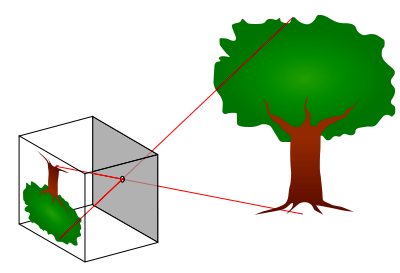
\includegraphics[scale=0.5, angle=0]{Files/Figures/pinhole3.png}
    \caption[Το μοντέλο κεντρικής προβολής (pinhole camera model)]{ Το μοντέλο κεντρικής προβολής (pinhole camera model) \cite{pinhole} .}
    \label{fig:pinhole3}
\end{figure}

\begin{figure}[H]
    \centering
    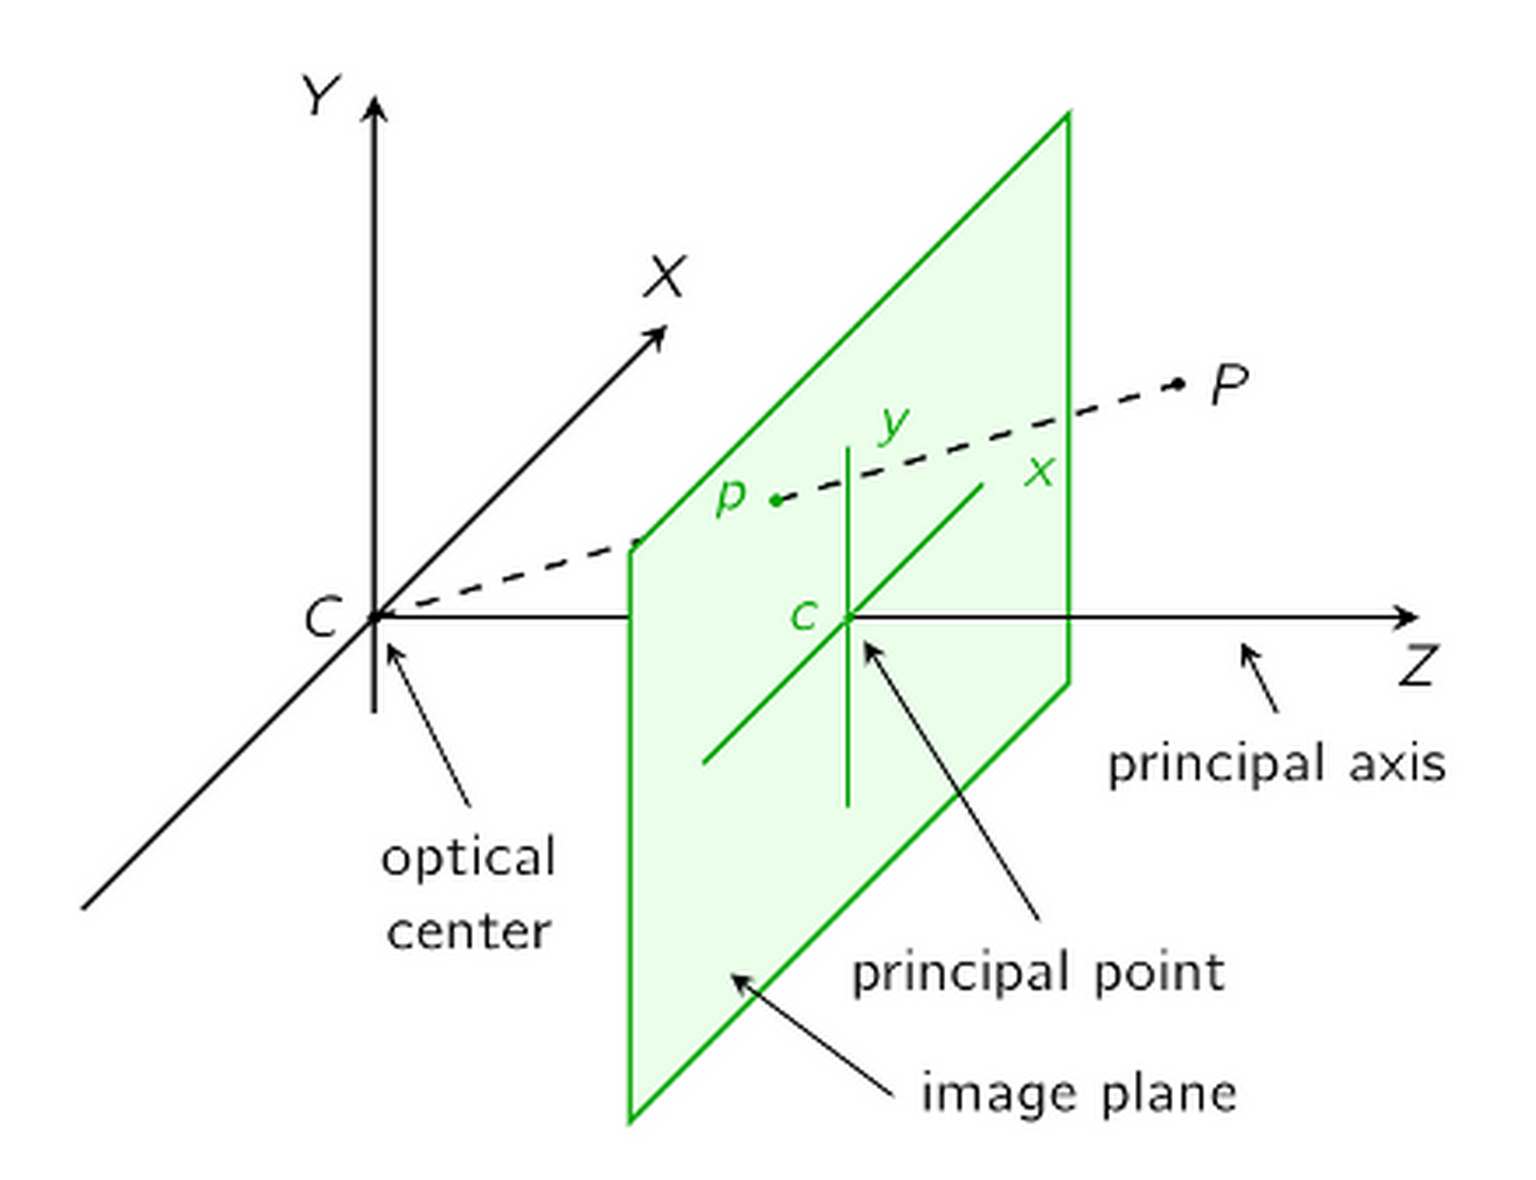
\includegraphics[scale=0.5, angle=0]{Files/Figures/pinhole1.png}
    \caption[Το μοντέλο κεντρικής προβολής (pinhole camera model)]{ Το μοντέλο κεντρικής προβολής (pinhole camera model) \cite{pinhole} .}
    \label{fig:pinhole1}
\end{figure}

\begin{figure}[H]
    \centering
    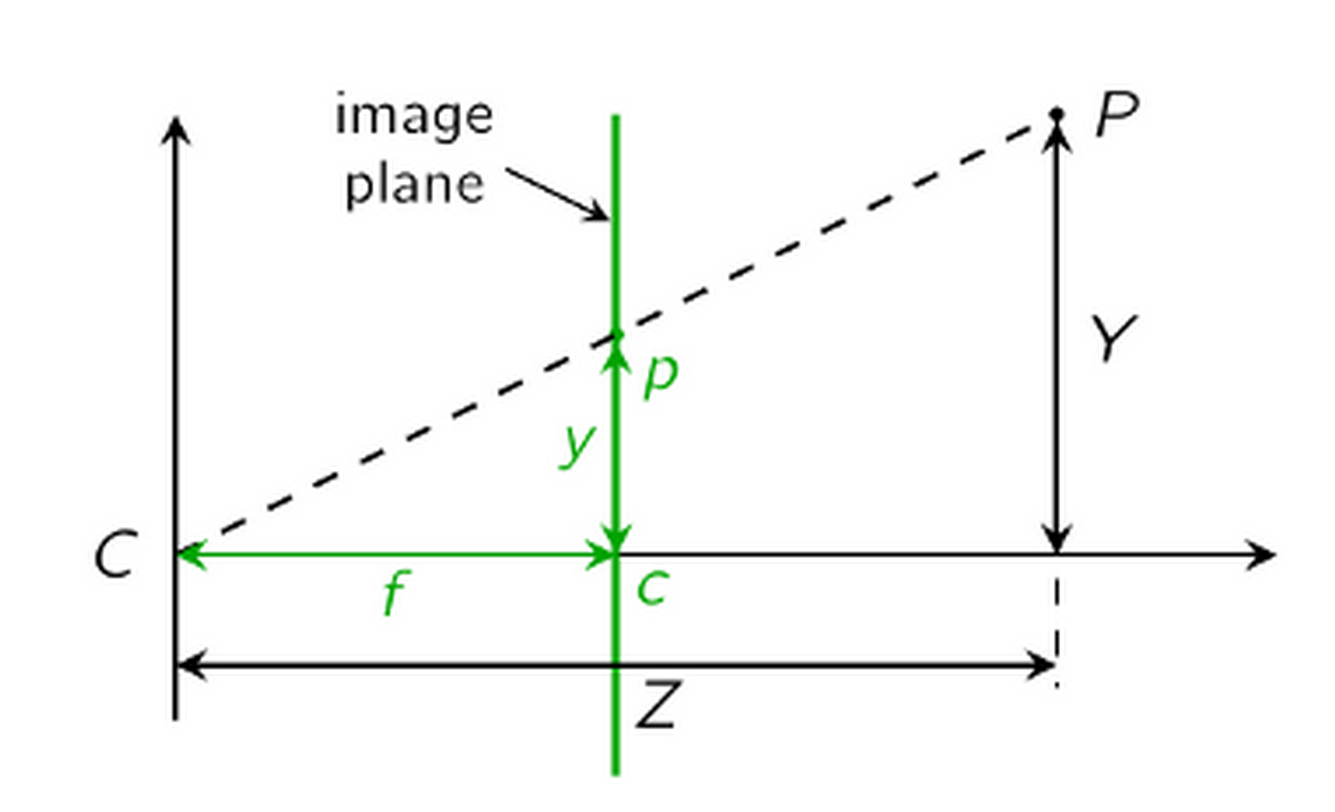
\includegraphics[scale=0.5, angle=0]{Files/Figures/pinhole2.png}
    \caption[Πλάγια όψη του μοντέλου κεντρικής προβολής (pinhole camera model)]{ Πλάγια όψη του μοντέλου κεντρικής προβολής (pinhole camera model) \cite{pinhole} .}
    \label{fig:pinhole2}
\end{figure}


\begin{figure}[H]
    \centering
    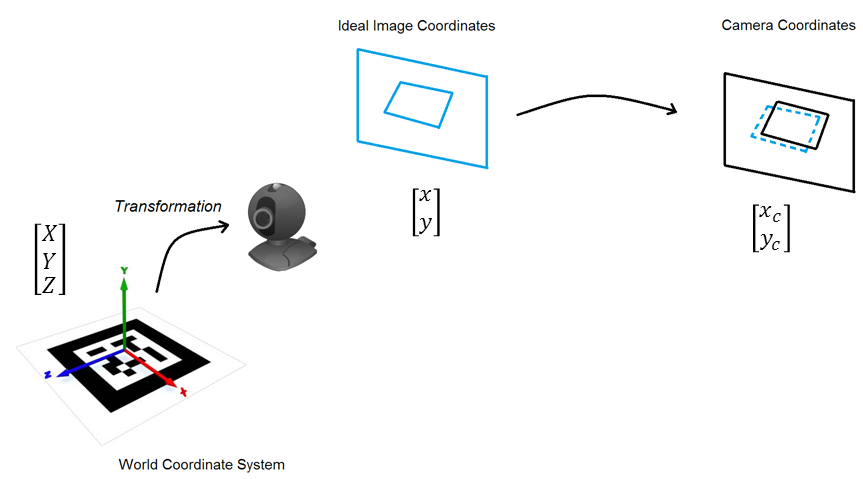
\includegraphics[scale=0.6, angle=0]{Files/Figures/transformation1.png}
    \caption[Στιγμιότυπο κατά τη διαδικασία της βαθμονόμησης κάμερας μέσω της OpenCV]{ Στιγμιότυπο κατά τη διαδικασία της βαθμονόμησης κάμερας μέσω της OpenCV}
    \label{fig:transformation1}
\end{figure}





%siltanen ta leei poli apla kai katanoita-exei lathi



%allo pinhole allo pragmatikes kameres!!!!!!
-camera calibration matrix and optical distortions
Τα φυσικά χαρακτηριστικά μιας κάμερας ορίζουν πώς θα διαμορφωθεί μία εικόνα στον αισθητήρα εικόνας μιας κάμερας. 

Ενώ στο μοντέλο pinhole, μόνο το εστιακό μήκος της κάμερας επηρεάζει τη διάταξη της εικόνας, στις πραγματικές κάμερες, ο αισθητήρας μπορεί να είναι ασύμμετρος, η αναλογία διαστάσεων pixel μπορεί να είναι ανόμοια και το κέντρο του αισθητήρα εικόνας $(c_{x},c_{y}$ μπορεί να διαφέρει σε απόσταση από τον οπτικό άξονα του συστήματος φακού.

Ένας τρόπος που χρησιμοποιείται, συνήθως, είναι η αναπαράσταση του μοντέλου της κάμερας ως ένας πίνακας βαθμονόμησης κάμερας (intrinsic camera calibration matrix) K, ή απλά πίνακας κάμερας (camera matrix). Πρόκειται για μία αντιστοίχηση ανάμεσα στις συντεταγμένες της ιδανικής 2D εικόνας και τις συντεταγμένες της εικόνας που απεικονίζεται στον αισθητήρα της κάμερας (observed pixel coordinates), $x_{pix}=Κx_{c}$. Επομένως, ο πίνακας βαθμονόμησης (calibration matrix) εξαρτάται μόνο από τις ιδιότητες της κάμερας.


\begin{equation}
\begin{bmatrix}
x_{pix} \\ y_{pix} \\ 1
\end{bmatrix}
=
\begin{bmatrix}
f_{x} & s & c_{x} & 0\\
0 & f_{y} & c_{y} & 0\\
0 & 0 & 1 & 0
\end{bmatrix}
\begin{bmatrix}
x_{c}\\
y_{c}\\
z_{c}
\end{bmatrix}
\end{equation} .

Επιπλέον, μία πραγματική κάμερα μπορεί να παράγει συστηματικά γεωμετρικά σφάλματα, που ονομάζονται παραμορφώσεις, λόγω ατελειών του φακού. 
Η παραμόρφωση αυτή συμβαίνει στο φακό της κάμερας. 
Επομένως, θεωρητικά, η παραμόρφωση πρέπει να ληφθεί υπόψη πριν γίνει ο μετασχηματισμός των ιδανικών συντεταγμένων σε συντεταγμένες κάμερας. 
Ωστόσο στις περισσότερες σύγχρονες κάμερες, τα pixels είναι τετράγωνα και οι στήλες και σειρές είναι ευθείες. Αυτό σημαίνει ότι στον πίνακα της κάμερας $s=0$, και $f_{x}=f_{y}$.

\begin{equation}
K=
\begin{bmatrix}
f & 0 & c_{x} & 0\\
0 & f & c_{y} & 0\\
0 & 0 & 1 & 0
\end{bmatrix}
\end{equation} .


%paramorfosi
Σε αυτή την περίπτωση, η παραμόρφωση μπορεί να μοντελοποιηθεί μετά μετά τον εσωτερικό μετασχηματισμό της κάμερας (camera’s intrinsic transformation). Ο πίνακας κάμερας μετατρέπει τις ιδανικές συντεταγμένες εικόνας σε συντεταγμένες κάμερας και έπειτα, η συνάρτηση παραμόρφωσης μετατρέπει τις συντεταγμένες κάμερας σε συντεταγμένες pixel.

\begin{equation}
D
\left(
\begin{bmatrix}
x_{c}\\
y_{c}   
\end{bmatrix}
\right )
=
\begin{bmatrix}
x_{pix}\\
y_{pix}   
\end{bmatrix}
\end{equation} 


\begin{equation}
D^{-1}
\left (
\begin{bmatrix}
x\\
y  
\end{bmatrix}
\right )
)=
\begin{bmatrix}
x_{c}\\
y_{c}
\end{bmatrix}
\end{equation} 


Η αντίστροφη συνάρτηση παραμόρφωσης $D^{-1}$, εξομαλύνει τις συντεταγμένες pixel σε συντεταγμένες κάμερας.




Η διαδικασία της βαθμονόμησης περιλαμβάνει, ουσιαστικά, την ταυτοποίηση των εσωτερικών παραμέτρων της κάμερας, δηλαδή του πίνακα κάμερας και την εκτίμηση της συνάρτησης παραμόρφωσης.


Οι εφαρμογές επαυξημένης πραγματικότητας συχνά χρησιμοποιούν ξεχωριστά εργαλεία βαθμονόμησης ή διενεργούν την διαδικασία βαθμονόμησης ξεχωριστά από την εφαρμογή. Συνήθως το εργαλείο βαθμονόμησης αποθηκεύει τα αποτελέσματα σε ένα αρχείο, το οποίο διαβάζει η εφαρμογή επαυξημένης πραγματικότητας. Από εδώ και στο εξής θα θεωρούμε ότι η συνάρτηση εξομάλυνσης (undistortion) $D^{-1}$ αι ο πίνακας βαθμονόμησης Κ είναι γνωστά. 


Συνοπτικά, ένα σύστημα εντοπισμού marker μπορεί να μετατρέψει τις συντεταγμένες εικόνας που παρατηρεί (pixel coordinates) μιας βαθμονομημένης κάμερας σε συντεταγμένες ιδανικής οθόνης. Οι συντεταγμένες pixel μετασχηματίζονται πρώτα σε συντεταγμένες κάμερας και μετά εξομαλύνονται:

\begin{equation}
K^{-1}D^{-1} 
\left (\begin{bmatrix}
x_{pix}\\ 
y_{pix}
\end{bmatrix}  \right )
=K_{-1}
\left (\begin{bmatrix}
x_{c}\\ 
y_{c}
\end{bmatrix}  \right )
=
\begin{bmatrix}
x\\ 
y
\end{bmatrix}
\end{equation}

Από την άλλη πλευρά, οι ιδανικές συντεταγμένες μπορούν να μετασχηματιστούν σε κοσμικές συντεταγμένες και αντίστροφα. Τέλος, μπορούμε να αναπαραστήσουμε τη σχέση ανάμεσα σε στις κοσμικές συντεταγμένες $X$ και τις παρατηρούμενες συντεταγμένες εικόνας $x_{pix}$,

\begin{equation}
K^{-1}D^{-1} 
\left (\begin{bmatrix}
x_{pix}\\ 
y_{pix}
\end{bmatrix}  \right )
=D
\left (KT \begin{bmatrix}
X\\ 
Y\\
Z
\end{bmatrix}  \right )
\end{equation}





%programming cv with python






Πέρα από την εστιακή απόσταση, οι μόνες παράμετροι είναι οι συντεταγμένες του οπτικού κέντρου(principal point), το σημείο εικόνας c = [cx, cy], όπου ο οπτικός άξονας τέμνει το επίπεδο της εικόνας. Εφόσον αυτό συνήθως συμβαίνει στο κέντρο της εικόνας και οι συντεταγμένες της εικόνας υπολογίζονται από την πάνω-αριστερή γωνία, αυτές οι τιμές μπορούν να προσεγγιστούν με το μισό μήκος και πλάτος της εικόνας.








%tzionas
Σαν μοντέλο κάμερας στην παρούσα εργασία επιλέγεται το pinhole μοντέλο, σε συνδυασμό με ορισμένες παραμέτρους που μοντελοποιούν κάποιες παραμορφώσεις.

-Απλό pinhole μοντέλο
Το pinhole μοντέλο είναι το απλούστερο μοντέλο κάμερας, το οποίο γίνεται μάλιστα και εύκολα κατανοητό μέσω του παραδείγματος της pinhole φωτογραφικής μηχανής (camera obscura) που μπορεί να κατασκευάσει κάποιος εύκολα.

Όπως βλέπουμε στην εικόνα, θεωρώντας την κάμερα σαν ένα κουτί με μία μικρή τρύπα στην "μπροστινή" επιφάνεια (χωρίς την ύπαρξη φακού), έχουμε τη δημιουργία μιας απλής φωτογραφικής μηχανής. Οι ακτίνες φωτός, αφού προσπέσουν πάνω σε ένα αντικέιμενο, περνάνε μέσα από την τρύπα της pinhole καμερας και καταλήγουν στην πισω επιφάνεια του κουτιού, όπου απεικονίζεται η τελική φωτογραφία που απεικονίζει τη σκηνή του πραγματικού κόσμου ανεστραμμένη.

Κατά τη φωτογράφιση έχουμε μία αποτύπωση του τρισδιάστατου περιβάλλοντος χώρου σε μία δισδιάστατη εικόνα μέσω του του φωτός, χάνοντας μάλιστα με τον τρόπο αυτό πληρφοροία από την πραγματική σκηνη (διατηρούνται οι γραμμές αλλά όχι τα σχήματα). Μία αναπαράσταση αυτής της αποτύπωσης-προβολής έχουμε στην παρακάτω εικόνα.


Όπως βλέπουμε, με αυτή τη νοητή μεταφορά έχουμε μία απλούστερη και πιο κατανοητή αναπατάσταση της διαδικασίας φωτογράφισης, καθώς πλέον δεν έχουμε ανεστραμμένη αποτύπωση των πραγματικών αντικειμένων στην εικόνα. Για λόγους απλούστευσης, χωρίς απώλεια της γενικότητας, θα διατηρηθεί αυτή η σύμβαση στο υπόλοιπο της εργασίας.

Μία πιο αυστηρή αναπαράσταση εμφανίζεται στην παρακάτω εικόνα.

Το σημείο pinhole που πάιζει και τον κεντρικό ρόλο στην όλη διαδικασία ονομάζεται και camera center ή optical center, ενώ το επίπεδο που περνάει από αυτό και είναι παράλληλο στο επίπεδο της εικόνα, δηλαδή το image plane, ονομάζεται principal plane (επίπεδο XCY). Ό άξονας που ξεκινά από το camera center και διαπερνά κάθετα το image plane ονομάζεται principal axis ενώ το σημείο τομής με το image plane ονομάζεται principal point.

Το image plane παριστάνεται με το επίπεδο 

\begin{equation}
 Z = f
\end{equation}

όπου f είναι η εστιακή απόσταση, ενώ η αποτύπωση-προβολή ενός πραγματικού σημείου σε αυτό γίνεται μέσω της τομής του ευθύγραμμου τμήματος XC με το επίπεδο του image plane.
Έαν τα σημεία του τρισδιάστατου πραγματικού χώρου παριστάνονται ως 

\begin{equation}
\hat{X}=
\begin{bmatrix}
X\\ 
Y\\ 
Z
\end{bmatrix}
\end{equation}

και τα σημεία του image plane ως


\begin{equation}
\hat{x}=
\begin{bmatrix}
f\frac{X}{Z}\\ 
f\frac{Y}{Z}
\end{bmatrix}
\end{equation}

τότε κατά την προβολή του 3D χώρου στο image plane έχουμε την αντιστοίχιση 


\begin{equation}
\begin{bmatrix}
X\\ 
Y\\ 
Z
\end{bmatrix}
\rightarrow
\begin{bmatrix}
f\frac{X}{Z}\\ 
f\frac{Y}{Z}
\end{bmatrix}
\end{equation}

Χρησιμοποιώντας ομογενείς συντεταγμένες η αντιστοίχιση σημείων παίρνει τη μορφή 

\begin{equation}
\begin{bmatrix}
X\\ 
Y\\ 
Z\\
1
\end{bmatrix}
\rightarrow
\begin{bmatrix}
fX\\ 
fY\\
Ζ
\end{bmatrix}
=
\begin{bmatrix}
f &  &  & 0\\ 
 & f & & 0\\
 & & 1 & 0
\end{bmatrix}
\begin{bmatrix}
X\\ 
Y\\
Z\\
1
\end{bmatrix}
\end{equation}

Θέτοντας 

\begin{equation}
\hat{X}=
\begin{bmatrix}
X\\ 
Y\\
Z\\
1
\end{bmatrix}
\end{equation}

και συμβολίζοντας με $\hat{x}$ το σημείο στο image plane, παίρνουμε την πιο κομψή αναπαράσταση αντιστοίχισης των σημείων

\begin{equation}
\hat{x}=P\hat{X}
\end{equation}

όπου ο πίνακας P μεγέθους 3x4 ονομάζεται και camera projection matrix

\begin{equation}
P=
\begin{bmatrix}
f & & & 0 \\
 & f &  & 0\\
 & & 1 & 0\
\end{bmatrix}
\end{equation}


-Σχετικά με το principal point
Στα προηγούμενα θεωρήθηκε ότι το σύστημα συντεταγμένων του image plane έχει την αρχή του στο principal point, κάτι που δεν ισχύει απαραίτητα. Έτσι πρέπει να τροποιηθεί το παραπάνω μοντέλο ώστε να ληφθεί υπόψη αυτή η μετατόπιση του συστήματος συντεταγμένων.

Εάν:

\begin{equation}
p=
\begin{bmatrix}
p_{x}\\
p_{y}
\end{bmatrix}
\end{equation}

είναι οι συντεταγμένες του principal point, με βάση τις προηγούμενες εξισώσεις

\begin{equation}
\begin{bmatrix}
X\\ 
Y\\
Z
\end{bmatrix}
\rightarrow
\begin{bmatrix}
f\frac{X}{Z}+p_{x}\\
f\frac{Y}{Z}+p_{y}
\end{bmatrix}
\end{equation}

\begin{equation}
\begin{bmatrix}
X\\ 
Y\\
Z\\
1
\end{bmatrix}
\rightarrow
\begin{bmatrix}
fX+Zp_{x}\\
fY+Zp_{y}\\
Z
\end{bmatrix}
=
\begin{bmatrix}
f & & p_{x} & 0\\
 & f & & p_{y} & 0\\
 & & 1 & 0
\end{bmatrix}
\end{equation}


\begin{equation}
K=
\begin{bmatrix}
f &  & p_{x}\\
 & f & p_{y}\\
 & & 1
\end{bmatrix}
\end{equation}

όπου ο 3x3 πίνακας Κ  ονομάζεται camera calibration matrix.


-Σχετικά με τα συστήματα συντεταγμένων
Κατά την προβολή του 3d κόσμου σε μία 2d εικόνα διαχειριζόμαστε σημεία που ανήκουν σε 2 διαφορετικά συστήματα συντεταγμένων

\begin{itemize}
\item Το σύστημα συντεταγμένων της κάμερας 
\item Το σύστημα συντεταγμένων του κόσμου (world coordinates system-WCS)
\end{itemize}


Ένα σημείο μπορεί να εκφραστεί με την κατάλληλη μορφή σε οποιοδήποτε από αυτά τα 2 συστήματα συντεταγμένων

Έτσι εαν:

\begin{itemize}
\item $\tilde{X}$ το ομογενές διάνυσμα ενός σημείου στο WCS
\item $\tilde{X_{cam}}$ το ομογενές διάνυσμα του ίδιου σημείου στο σύστημα συντεταγμένων της κάμερας
\item $\tilde{C}$ οι συντεταγμένες του κέντρου της κάμερας στο WCS
\item R ο πίνακας 3x3 Rotation
\end{itemize}

Έχουμε:

\begin{equation}
\tilde{X_{cam}}=R(\tilde{X}-\tilde{C})
\end{equation}

Ενώ αν θέσουμε 


\begin{equation}
t=-R\tilde{C}
\end{equation}


Έχουμε 

\begin{equation}
\tilde{X_{cam}}=R\tilde{X}+t
\end{equation}


και ο πίνακας προβολής είναι

\begin{equation}
P=K[R|t]
\end{equation}


Ο πίνακας rotation R περιγράφει τον προσανατολισμό του συστήματος συντεταγμένων της κάμερας. Η συνολική περιστροφή που περιγράφει αυτός ο πίνακας 3x3 εκτελείται μέσω των στοιχειωδών περιστροφών που ορίζουν οι τρεις στήλες με την παρακάτω σειρά.


\begin{itemize}
\item η πρώτη στήλη περιστρέφει το αρχικό σύστημα συντεταγμένων ως προς τον άξονα x
\item η δεύτερη στήλη περιστρέφει το ήδη περιστραμμένο σύστημα ως προς τον άξονα  y
\item η τρίτη στήλη περιστρέφει το ήδη δις περιστραμμένο σύστημα ως προς τον άξονα  z 
\end{itemize}



-Παραμορφώσεις αισθητήρα κάμερας
Πριν φτάσει η κατασκευή των αισθητήρων στο σημερινό επίπεδο, ο αισθητήρας εισήγαγε ορισμένες παραμορφώσεις στο μοντέλο της κάμερας.

Έτσι αν:

\begin{itemize}
\item s(skew) είναι η γωνία των δύο πλευρών του κάθε pixel του αισθητήρα (που
μπορεί με αυτό τον τρόπο να μην έχουν ορθογώνιο σχήμα αλλά απλά παραλληλόγραμο),
\item και το εστιακό μήκος δίνεται λόγω των άνισων πλευρών του καθε pixel από τους τύπους
\end{itemize}


\begin{equation}
f_{x}=fm_{x}
\end{equation}
\\
\begin{equation}
f_{y}=fm_{y}
\end{equation}

τότε ο πίνακας calibration matrix δίνεται από τη σχέση 


\begin{equation}
Κ=
\begin{bmatrix}
f_{x} & s & x_{0}\\
 & f_{y} & y_{0}\\
 & & 1
\end{bmatrix}
\end{equation}


Σήμερα ωστόσο οι αισθητήρες μπορεί να θεωρηθεί ότι έχουν τα pixels τους αισθητήρα ορθογώνια, επομένως το s είναι συνήθως μηδενικό. 


-Σχετικά με το φακό
Προσθέτοντας στο μοντέλο της κάμερας το φακό που έχουν όλες οι κάμερες, εισάγονται αυτόματα οι παραμορφώσεις των οπτικών στοιχείων. Ανάλογα με την ποιότητα της κάμερας διαφέρει και το μέγεθος των παραμορφώσεις.

Συμβολίζοντας με :

\begin{equation}
f_{xy}=
\begin{bmatrix}
f_{x}\\
f_{y}
\end{bmatrix} το εστιακό μήκος
\end{equation}
\\
\begin{equation}
p=
\begin{bmatrix}
p_{x}\\
p_{y}
\end{bmatrix} το principal point
\end{equation}
\\
s το skew\\
$k_{c}$ ένα 5x1 διάνυσμα που μοντελοποιεί τις ακτινικές και εφαπτομενικές παραμορφώσεις

αν ένα σημείο του χώρου παριστάνεται ως προς το σύστημα συντεταγμένων της κάμερας ως:

\begin{equation}
\tilde{X_{cam}}=
\begin{bmatrix}
X_{cam}\\
Y_{cam}\\
Z_{cam}
\end{bmatrix}
\end{equation}

η προβολή του στο image plane θα είναι το κανονικοποιημένο διάνυσμα 

\begin{equation}
x_{n}=
\begin{bmatrix}
\frac{X_{cam}}{Z_{cam}}\\
\frac{Y_{cam}}{Z_{cam}}
\end{bmatrix}
\end{equation}

Θέτοντας

\begin{equation}
r^{2}=x^{2}+y^{2}
\end{equation}

το παραπάνω κανονικοποιημένο διάνυσμα παίρνει την παρακάτω μορφή που συμπεριλαμβάνει την επίδραση των παραμορφώσεων


\begin{equation}
x_{d}=
\begin{bmatrix}
x_{d}(1)\\
x_{d}(2)
\end{bmatrix}
=
(1+k_{c}(1)\cdot r^{2}+k_{c}(2)\cdot r^{4}+k_{c}(5)\cdot r^{6})x_{n}+d_{x}
\end{equation}


όπου 

\begin{equation}
x_{d}=
\begin{bmatrix}
2k_{c}(3)\cdot xy+k_{c}(4)(r^{2}+2x^{2})\\
2k_{c}(4)\cdot xy+k_{c}(3)(r^{2}+2y^{2})
\end{bmatrix}
\end{equation}

Έχοντας μοντελοποιήσει τις παραμορφώσεις, η αντιστοίχιση που περιγράφεται παίρνει πλέον τη μορφή

\begin{equation}
\begin{bmatrix}
x_{p}\\
y_{p}\\
1
\end{bmatrix}
=
K
\begin{bmatrix}
x_{d}(1)\\
y_{d}(2)\\
1
\end{bmatrix}
\end{equation}


όπου 

\begin{equation}
K=
\begin{bmatrix}
f_{x} & s\cdot f_{x} & p_{x}\\
0 & f_{y} & p_{y}\\
0 & 0 & 1
\end{bmatrix}
\end{equation}

Ωστόσο συνήθως θεωρούμε 

\begin{itemize}
\item $s=0$, θεωρώντας με ασφάλεια ότι έχουμε ορθογώνια pixels αισθητήρα
\item $k_{c}(5)=0$, όταν έχουμε φακούς περίπου κανονικής εστιακής απόστασης (και όχι αρκετά ευρυγώνιους)
\end{itemize}

Στην περίπτωση που η κάμερα μοντελοποιείται χωρίς παραμορφώσεις από τον φακό, έχουμε ότι:

\begin{equation}
K=
\begin{bmatrix}
x_{p}\\
y_{p}\\
1
\end{bmatrix}
=K
\begin{bmatrix}
x_{n}(1)\\
y_{n}(2)\\
1
\end{bmatrix}
\end{equation}


%mcdonald
Το μοντέλο κάμερας pin-hole χρησιμοποιείται συχνά στην υπολογιστική όραση και τα γραφικά υπολογιστών για την μοντελοποίηση της προβολικής μετρατοπής μίας τρισδιάστατης σκηνής σε ένα δισδιάστατο επίπεδο προβολής \cite{hartley2003multiple} .

Η εικόνα Figure 3.1 [ROTH99] δείχνει το μοντέλο της κάμερας, όπου ο φακός της βρίσκεται στην αρχή των αξόνων (origin) και ένα σημείο p προβάλλεται πάνω στο φωτογραφικό φιλμ και συγκεκριμένα πάνω στο σημείο p'. Η απόσταση ανάμεσα στο φωτογραφικό φιλμ και το φακό ονομάζεται εστιακή απόσταση και επισημαίνεται ως d.


Χρησιμοποιώντας το συγκεκριμένο μοντέλο, μπορούμε να ορίσουμε μία σχέση ανάμεσα στις τρισδιάστατες συντεταγμένες της εικονικής σκηνής, x, y, z και τις συντεταγμένες x', y' της δισδιάστατης εικόνας. 

\[ x' = d  \frac{x}{z}\] και \[ y' = d  \frac{y}{z}\]

Σε μία πιο γενική μορφή, η σχέση αυτή μπορεί να αναπαρασταθεί με τον παρακάτω τρόπο σε ομογενή μετασχηματισμό.

\[ p' = Mp\] 

όπου p και p’ είναι ομογενή σημεία και το M είναι ένας πίνακας προβολής 4x4, ο οποίος μπορεί να γραφτεί ως:


\begin{equation}
C(f) \leq n + 1 = O(n).
\end{equation}


\begin{equation}
\begin{bmatrix}
x\\ 
y\\ 
z\\ 
w
\end{bmatrix}
=
\begin{bmatrix}
0 & 0 & 0 & 0 \\ 
0 & 0 & 0 & 0 \\ 
0 &  0  & 0  & 0 \\ 
0 & 0  & 0 & 0
\end{bmatrix}
\begin{bmatrix}
x'\\ 
y'\\ 
z'\\ 
w
\end{bmatrix}
\end{equation}


Για να πάρουμε το συγκεκριμένο πίνακα προβολής για μία αυθαίρετη θέση της κάμερας στο χώρο, πρέπει να υπολογιστούν ανεξάρτητα οι εσωτερικές και οι εξωτερικές παράμετροι της κάμερας. 




\subsection{Παράμετροι Κάμερας}

Υπάρχουν δύο υποσύνολα παραμέτρων κάμερας που μπορούν να χρησιμοποιηθούν προκειμένου να καθοριστεί η σχέση ανάμεσα στα συστήματα συντεταγμένων.
Γνωστά ως εσωτερικές και εξωτερικές παράμετροι στο πεδίο της όρασης υπολογιστών, ορίζονται ως:



-Intrinsics-


%malik
Οι εσωτερικές παράμετροι είναι αυτές που σχετίζονται με την εσωτερική γεωμετρία μίας κάμερας. Με άλλα λόγια αναπαριστούν τα οπτικά, γεωμετρικά και ψηφιακα χαρακτηριστικά μιας κάμερας και είναι οι:

\begin{itemize}
\item Το εστιακό μήκος
\item Η θέση του κέντρου της εικόνας στο pixel space
\item Το μέγεθος pixel στις οριζόντιες και κάθετες κατευθύνσεις
\item οι παραμορφώσεις του φακού
\end{itemize}

The focal length
2) The location of the image center in pixel space
3) The pixel size in the horizontal and vertical directions
4) Ο συντελεστής λόγω της ακτινικής παραμόρφωσης.




%tzionas
Οι εσωτερικές παράμετροι που ορίζουν την αντιστοίχιση των συντεταγμένων στο σύστημα συντεταγμένων της εικόνας (2D) και στο σύστημα συντεταγμένων της κάμερας είναι:

\begin{itemize}
\item Το εστιακό μήκος
\item Η θέση του principal point
\item Ο συντελεστής s σχετικά με το σχήμα των pixels του αισθητήρα
\item οι παραμορφώσεις του φακού
\end{itemize}





%mcdonald
Οι εσωτερικές παράμετροι της κάμερας που πρέπει να υπολογιστούν είναι η εστιακή απόσταση, η θέση του κέντρου της εικόνας (principle point) στο χώρο των pixels, η αναλογία των διαστάσεων και ένας συντελεστής της ακτινικής παραμόρφωσης \cite{Malik2002}. 



Το κέντρο της εικόνας και η αναλογία των διαστάσεων περιγράφουν τη σχέση ανάμεσα στις συντεταγμένες εικόνας-χώρου(x', y') και τις συντεταγμένες της κάμερας (x,y) που δίνονται από τις σχέσεις:

\begin{equation}
\begin{aligned}
x=-(x'-o_{x})s_{x}
\\
y=-(y'-o_{y})s_{y}
\end{aligned}
\end{equation}

Οι μεταβλητές $(o_{x},o_{y})$ αναπαριστούν τις συντεταγμένες pixel του principal point, ενώ οι μεταβλητές (sx,sy) το μέγεθος των pixels (σε χιλιοστά) στην οριζόντια και τη κάθετη κατεύθυνση αντίστοιχα.
Συνήθως η ακτινική παραμόρφωση μπορεί να αγνοηθεί, εκτός κι αν κρίνεται απαραίτητη η υψηλή ακρίβεια σε όλα τα μέρη της εικόνας. 


-Extrinsics-

%siltanen
Οι εξωτερικές παράμετροι ορίζουν τη θέση και το προσανατολισμό της κάμερας ( ή ακριβέστερα του συστήματος συντεταγμένων της κάμερας σε σχέση με τις κοσμικές συντεταγμένες της σκηνής). Αυτός ο μετασχηματισμός M αποτελείται από μία συνιστώσα περιστροφής R και μία συνιστώσα μετατόπισης t, οι οποίες περιγράφονται σε κοσμικές συντεταγμένες (world coordinates) παρακάτω:



Ο μετασχηματισμός M ανάμεσα σε μία κάμερα και έναν marker είναι

\begin{equation}
\textbf{x=M\!X}
\end{equation}


όπου $\textbf{Χ}$ είναι ένα σημείο σε συντεταγμένες κόσμου, $\textbf{x}$ είναι η προβολή του σημείου σε συντεταγμένες ιδανικής εικόνας και M είναι ο μετασχηματισμός ανάμεσα σε κάμερα και marker, ή αλλιώς extrinsic camera matrix ή πίνακας πόζας. R είναι ένας πίνακας περιστροφής  και t ένα.

Ο μετασχηματισμός M αποτελείται από ένα  3Δ διάνυσμα μετατόπισης που περιγράφει τη θέση του κέντρου της κάμερας και από ένα πίνακα 3x3 R περιστροφής που περιγράφει τον προσανατολισμό της κάμερας. Ο μετασχηματισμός μπορεί να οριστεί σε μορφή πίνακα ως 


\begin{equation}
\textbf{x}=
\begin{bmatrix}
\textbf{R \! | \! t}
\end{bmatrix}
\textbf{X}
\end{equation}


ή σε ομογενείς συντεταγμένες :

\begin{equation}
\begin{bmatrix}
x \\ y \\ z
\end{bmatrix}
=
\begin{bmatrix}
r_{1} & r_{2} & r_{3} & t_{x}\\
r_{4} & r_{5} & r_{6} & t_{y}\\
r_{7} & r_{8} & r_{9} & t_{z}
\end{bmatrix}
\begin{bmatrix}
X\\
Y\\
Z\\
1
\end{bmatrix}
\end{equation}

Όπως είναι γνωστό, ένας πίνακας περιστροφής έχει μόνο τρεις παραμέτρους $(\alpha, \beta, \gamma)$ οι οποίες ορίζουν τα 9 στοιχεία του. Ένα διάνυσμα μετατόπισης έχει επίσης 3 παραμέτρους και επομένως ο πίνακας πόζας έχει 6 ελεύθερες παραμέτρους. Ένα σύστημα εντοπισμού marker πρέπει να λύνει αυτό τον πίνακα (camera matrix) σε κάθε frame, όταν ανιχνεύει έναν marker.









\subsection{Βαθμονόμηση Κάμερας}
%Η ΔΙΑΔΙΚΑΣΙΑ ΒΑΘΜΟΝΟΜΗΣΗΣ ΚΑΙ ΓΕΝΙΚΑ Η ΘΕΩΡΙΑ ΑΠΟ ΠΙΣΩ(ΤΟ ΠΩς ΓΙΝΕΤΑΙ ΣΤΟ ΚΕΦΑΛΑΙΟ 4)



%clarke
Η εύρεση των εσωτερικών παραμέτρων της κάμερας είναι γνωστή ως βαθμονόμηση κάμερας ή camera calibration και στόχο έχει τον προσδιορισμό των στοιχείων του εσωτερικού προσανατολισμού της κάμερας από δισδιάστατες εικόνες. Αυτές περιλαμβάνουν την εστιακή απόσταση, το "principal point" και την αναλογία των διαστάσεων (aspect ratio). 

Η συνολική απόδοση μιας εφαρμογής επαυξημένης πραγματικότητας, εξαρτάται άμεσα από την ακρίβεια της βαθμονόμησης της κάμερας. 


%%tzionas
 Παρά το γεγονός ότι το αντικείμενο παρουσιάζει ιδιαίτερο ερευνητικό ενδιαφέρον, δεν είναι στους στόχους της εργασίας η περαιτέρω ανάλυσή του. Στα πλαίσια της διπλωματικής εργασίας απαιτείται η χρήση μιας απλής μεθόδου με αξιοποίηση συνηθισμένου εξοπλισμού για την βαθμονόμηση. 


%σκακιερα
Καταφεύγουμε λοιπόν, στη λύση του εργαλείου της Opencv για την βαθμονόμηση της κάμερας[80], που προσφέρει μία έτοιμη και αποτελεσματική λύση, με χρήση μίας απλής κάμερας και μιας απλής επίπεδης εικόνας και συγκεκριμένα του μοτίβου τετραγώνων σκακιέρας, η οποία χρειάζεται απλά να εκτυπωθεί σε απλό χαρτί. 
Γενικά, η βαθμονόμηση μέσω της καταγραφής πολλαπλών λήψεων ενός επίπεδου αντικειμένου με χαρακτηριστικά σημεία, όπως είναι η σκακιέρα, επιτυγχάνεται με δεδομένα τις συντεταγμένες χώρου και εικόνας των αντίστοιχων σημείων, οι πρώτες εκ των οποίων προκύπτουν αυτόματα, ενώ οι τελευταίες αναγνωρίζονται στην εικόνα ομοίως με αυτόματο τρόπο. Ωστόσο, για την εξασφάλιση σωστών αποτελεσμάτων από τη διαδικασία της βαθμονόμησης, οι εικόνες του αντικειμένου πρέπει να ληφθούν από διαφορετικά σημεία και υπό διαφορετικές γωνίες. 




Αυτό το οποίο θα πρέπει να συγκρατήσει ο αναγνώστης, είναι ότι μέσω της διαδικασίας της βαθμονόμησης παίρνουμε τις εσωτερικές παραμέτρους της κάμερας μέσω μιας offline διαδικασίας που πραγματοποιείται μόνο μία φορά στην αρχή της διαδικασίας ανάπτυξης της εφαρμογής. Οι παράμετροι που υπολογίζονται, ορίζονται ως είσοδος στην εφαρμογή που θα αναπτυχθεί, προκειμένου να λειτουργήσει σωστά. Επομένως, δε χρειάζεται να πραγματοποιείται βαθμονόμηση κάθε φορά πριν ξεκινήσει μία εφαρμογή επαυξημένης πραγματικότητας. Αρκεί να γίνει μόνο μία φορά στην αρχή, εκτός και αν τα αποτελέσματα δεν έχουν αρκετή ακρίβεια. Ωστόσο αν σε ένα σύστημα επαυξημένης πραγματικότητας χρησιμοποιηθεί διαφορετική κάμερα, τότε πρέπει να γίνει εκ νέου βαθμονόμηση για τη νέα κάμερα.






\subsection{Ανίχνευση Marker}



\begin{figure}[H]
    \centering
    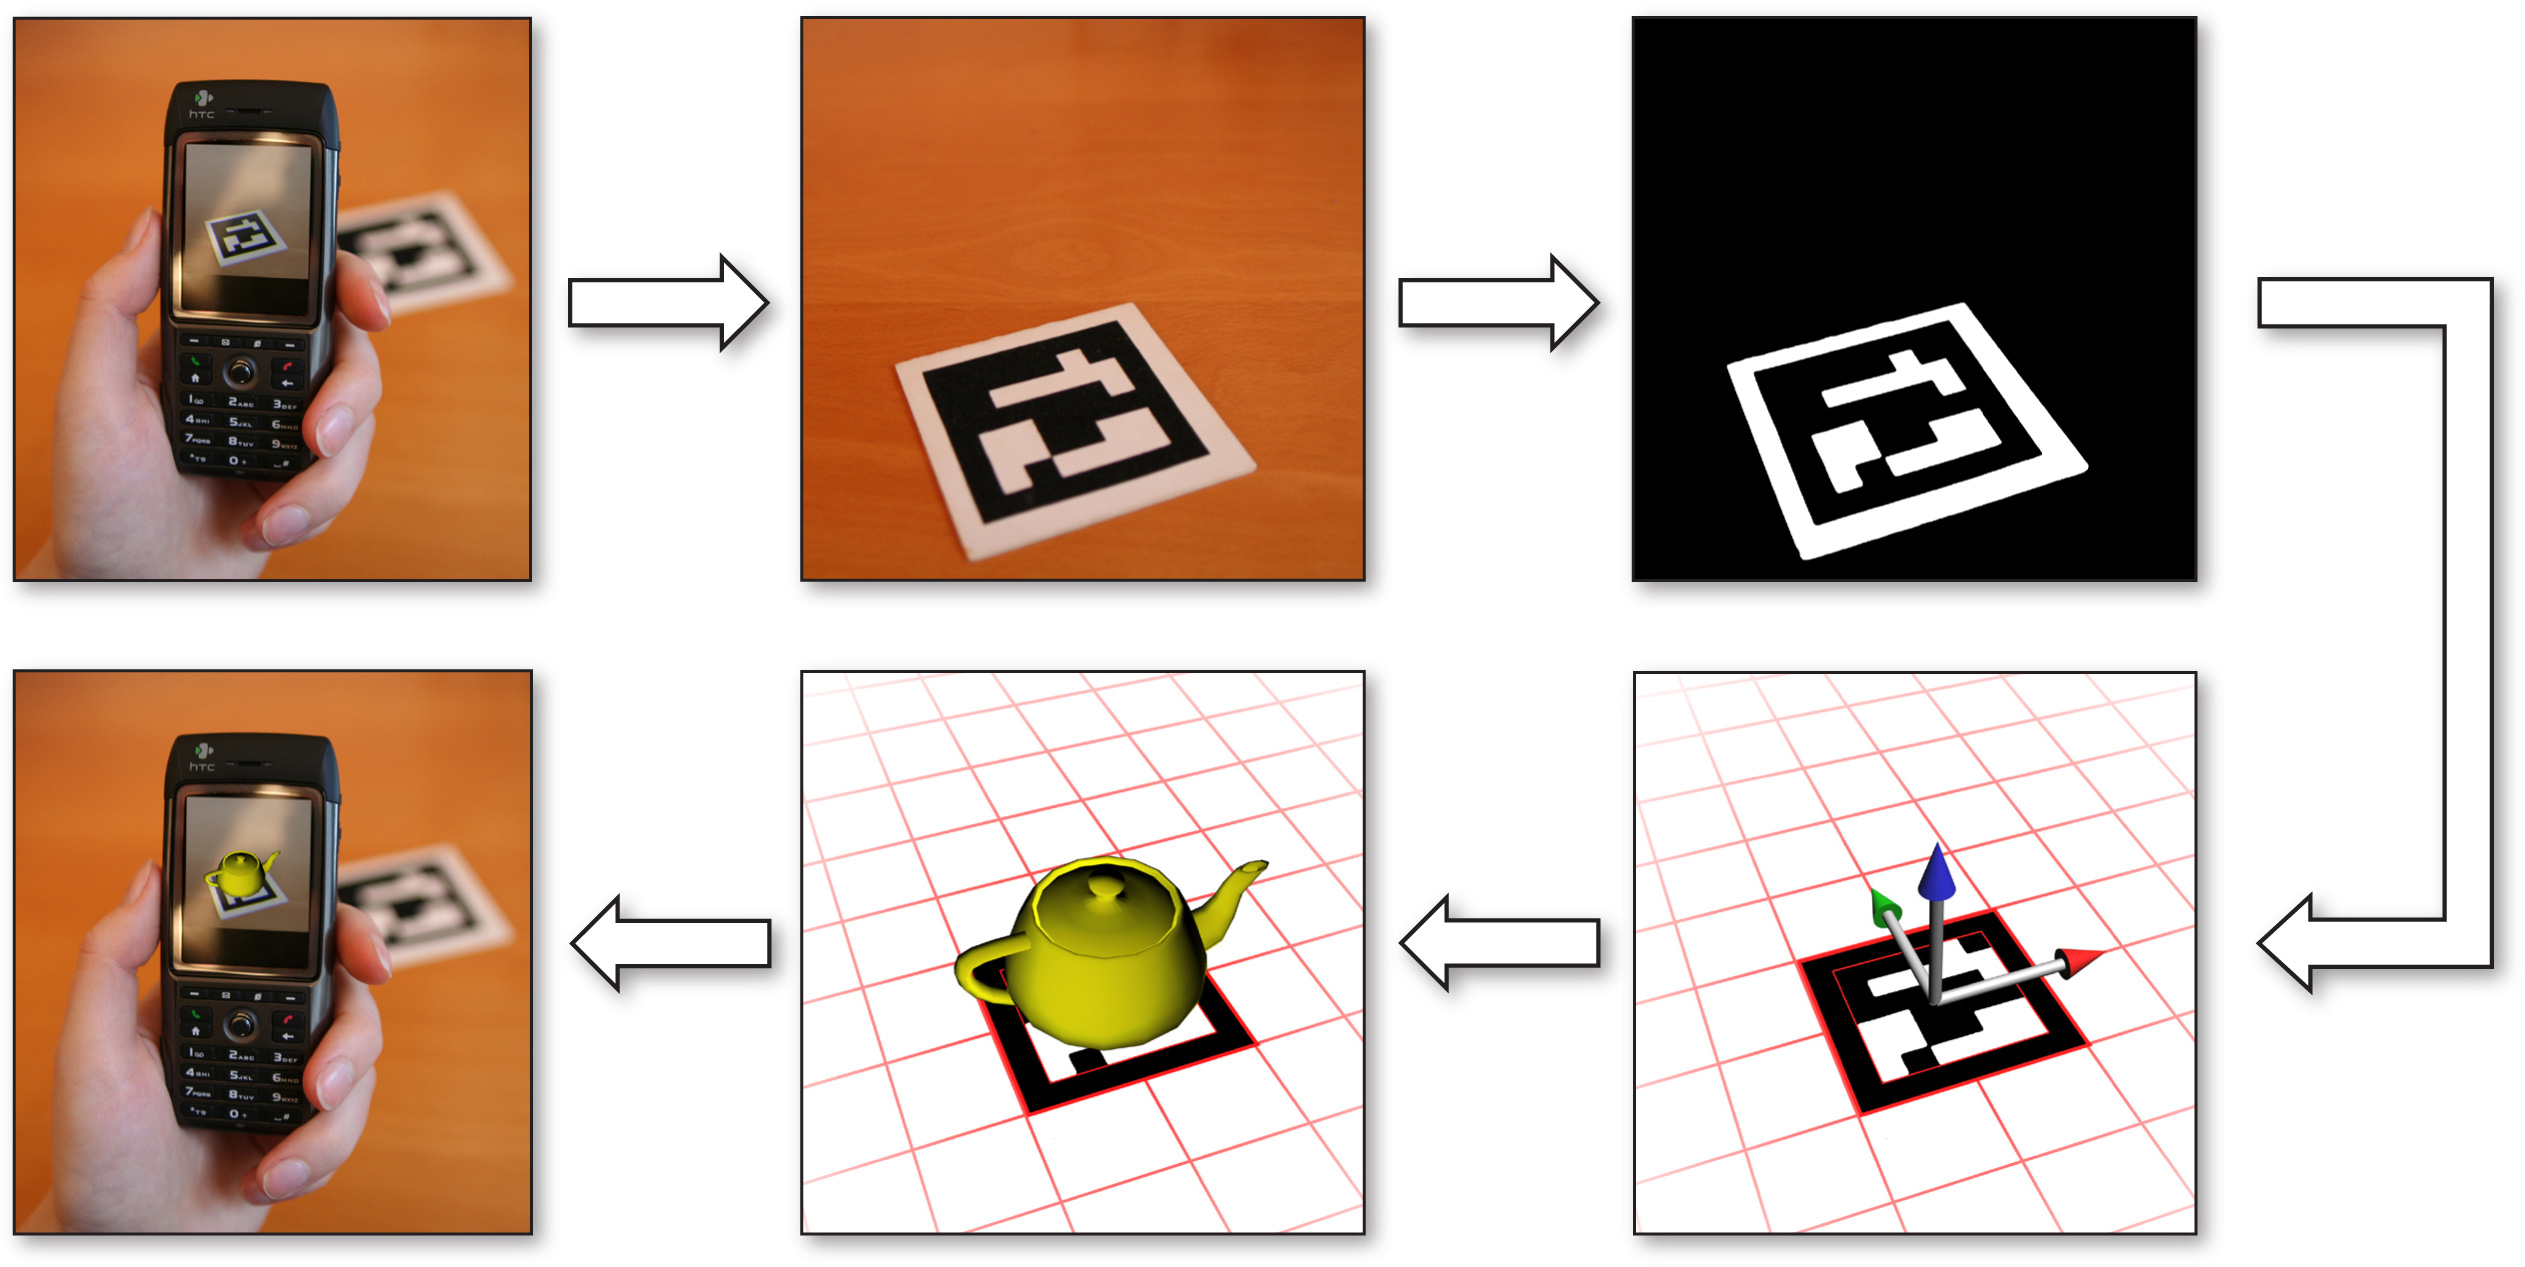
\includegraphics[scale=0.6, angle=0]{Files/Figures/HowMarkersWork.jpg}
    \caption[Παράδειγμα εντοπισμού marker και επαύξησης της σκηνής \cite{howmarkerswork}]{ Παράδειγμα εντοπισμού marker και επαύξησης της σκηνής \cite{howmarkerswork}}
    \label{fig:howmarkerswork}
\end{figure}


%siltanen
Ένας καλός marker πρέπει να μπορεί να ανιχνευθεί εύκολα και αξιόπιστα κάτω από όλες τις συνθήκες. Ορισμένες διαφορές στην φωτεινότητα(luminance) εντοπίζονται ευκολότερα από διαφορές στο χρώμα (colour) αν χρησιμοποιηθούν τεχνικές όρασης υπολογιστών \cite{hartley2003multiple} . Επιπλέον, ο φωτισμός αλλάζει τα αντιληφθέντα χρώματα των αντικειμένων και εποένως η ανίχνευση χρώματος είναι δύσκολη. Φυσικά, όσο περισσότερη αντίθεση φωτισμού υπάρχει, τόσο ευκολότερα εντοπίζονται αντικείμενα. Με αυτή την έννοια, η χρήση ασπρόμαυρων markers βελτιστοποιεί την διαδικασία ανίχνευσης. Το σύστημα πρέπει επίσης να μπορεί να υπολογίζει την πόζα της κάμερας με βάση το marker που εντοπίστηκε. Για να συμβεί αυτό, αρκεί να υπολογιστούν 4 σημεία και έτσι μπορούμε να υπολογίσουμε την μία και μοναδική λύση για την πόζα της κάμερας και ο ευκολότερος τρόπος για να συμβεί αυτό είναι η χρήση του σχήματος τετραγώνου για τα markers. Επιπλέον, οι θέσεις των γωνιακών σημείων είναι γενικά εύκολο να υπολογιστούν, καθώς αποτελούν ουσιαστικά την τομή των ακραίων ακμών ενός marker. Συμπερασματικά, τα περισσότερα συστήματα χρησιμοποιούν ασπρόμαυρους δείκτες και για αυτό το λόγο θα επεξηγηθεί στη συνέχεια η διαδικασία εντοπισμού ασπρόμαυρων markers.    




%des siltanen gia marker detection procedure


-diadikasia marker detection
Ο πρωταρχικός στόχος, επομένως, μιας διαδικασίας ανίχνευσης marker είναι η εύρεση των περιγραμμάτων πιθανών markers και μετέπειτα η εξαγωγή των γωνιών τους στην εικόνα. Επιπλέον, το σύστημα ανίχνευσης πρέπει να εξακριβώσει ότι αυτό που βρέθηκε είναι όντως marker και να αποκωδικοποιήσει την ταυτότητα του. Τέλος το σύστημα υπολογίζει την πόζα, με βάση τις πληροφορίες από τη θέση στην οποία ανιχνεύθηκε ο marker.

Τα βασικά βήματα ανίχνευσης είναι τα παρακάτω:
\begin{itemize}


\item Image acquisition
Απόκτηση μίας εικόνας έντασης
δcquisition of an intensity image.
\item Preprocessing-Προεπεξεργασία
Επεξεργασία εικόνας σε χαμηλό επίπεδο-low level image processing
Αντιστροφή της Παραμόρφωσης(undistortion)
Ανίχνευση ακμών και προσαρμογή ακμών
Ανίχνευση γωνιών marker

Πριν από την πραγματική ανίχνευση ενός marker, το σύστημα πρέπει να πάρει μία εικόνας έντασης (greyscale image). Aν το format της εικόνας που καταγράφηκε είναι άλλου τύπου, πχ RGB, τότε θα μετασχηματιστεί σε εικόνας κλίμακας γκρι χρησιμοποιώντας μία γνωστές τεχνικές \cite{Gonzalez}. 
Πρώτος στόχος είναι η ανίχνευση των ορίων πιθανών markers. Συνήθως είτε γίνεται πρώτα κατωφλίωση της εικόνας και μετά αναζήτηση για markers από τη δυαδική εικόνα, ή γίνεται ανίχνευση ακμών από την εικόνα κλίμακας του γκρι. Αυτές οι μέθοδοι επεξεργασίας χαμηλού επιπέδου(thresholding,
edge detection, line fitting, etc.) είναι γνωστές και επομένως δε θα αναλυθούν περαιτέρω στη συγκεκριμένα εργασία. Ωστόσο οι αναγνώστες μπορούν να ανατρέξούν στα \cite{Gonzalez}, \cite{szeliski2010computer}, για περισσότερα παραδείγματα.

Τα συστήματα τα οποία χρησιμοποιούν προσεγγίσεις κατωφλίωσης, συνήθως χρησιμοποιούν μεθόδους προσαρμοστικής κατωφλίωσης (e.g. [75]) ώστε να αντιμετωπίσουν τις τοπικές αλλαγές φωτεινότητας. Μετά την κατωφλίωση το σύστημα έχει μία δυαδική εικόνα που αποτελείται από το παρασκήνιο και τα αντικείμενα. Όλα τα αντικείμενα είναι πιθανοί υποψήφιοι markers σε αυτό το στάδιο. Συνήθως η επόμενη φάση είναι η επισήμανσή τους ή η συνεχής ανίχνευση τους. Κατά τη διαδικασία επισήμανσης το σύστημα μπορεί να απορρίψει αντικείμενα τα οποία είτε είναι πολύ μικρά είτε είναι οτιδήποτε άλλο εκτός από marker. Τέλος οι ακμές όλων των πιθανών markers επισημαίνονται και οι θέσεις τους εξομαλύνονται(undistort) για το στάδιο του line fitting (Figure 26). Έπειτα, το σύστημα εξετάζει και πάλι πιθανά markers, ελέγχοντας αν έχουν 4 ευθείες γραμμές και 4 γωνίες. Τέλος, το σύστημα βελτιστοποιεί τις θέσεις των γωνιών με ακρίβει sub-pixel. Figure 27 δείχνει το σύστημα συντεταγμένων του marker και την μία επαύξηση ακριβώς από πάνω του.
Η ανίχνευση ακμών σε εικόνες κλίμακας του γκρι είναι μία διαδικασία που παίρνει αρκετό χρόνο και επομένως τα συστήματα συνήθως χρησιμοποιούν υποδειγματοληψία και ανιχνεύουν ακμές μόνο σε ένα προκαθορισμένο πλέγμα. Αυτή η προσέγγιση οδηγεί σε ξεχωριστά σημεία γραμμών, το σύστημα πρέπει να συνδέσει τα pixels των ακμών σε τμήματα, αξιοποιώντας την τεχνική edge sorting. As the system samples the
original points using a coarse grid, it needs to extend the lines to full length to find the exact corners of the marker. A common procedure is to use the gradient  information of the original image to extend the edges to full length.

Συνήθως οι εικόνες δεν είναι παραμορφωμένες, αφού χρησιμοποιείται η αντίστροφη διαδικασία παραμόρφωσης η οποία υπολογίστηκε κατά τη διαδικασία της βαθμονόμησης. Ωστόσο στα συστήματα πραγματικού χρόνου, εξομαλύνονται μόνο οι θέσεις των σημείων χαρακτηριστικών, π.χ οι ακμές ενός marker που ανιχνεύθηκαν για να επιταχυνθεί η διαδικασία. Η διαδικασία της βαθμονόμησης αναλύεται σε επόμενη ενότητα.

Ακόμα και μικρά λάθη σε εντοπισμένες δισδιάστατες θέσεις ακμών και γωνιών επηρεάζουν την πόζα της κάμερας όταν υπολογίζεται. [77–79]. Λάθη ανίχνευσης μπορεί να συμβούν λόγω σφάλματος κβαντοποίησης pixel, λαθασμένης τιμής ορίου κατωφλίωσης, θολώματος κίνησης, θορύβου κλπ. Αυτά τα σφάλματα προκαλούν ενοχλητικό τρέμουλο (jitter) στην πόζα ενός αντικειμένου, ακόμα και αν η κάμερα κινείται ελάχιστα. 
Για να βελτιωθεί η ακρίβεια, τα συστήματα βελτιστοποιούν τις θέσεις μετά την αρχική ανίχνευση.


\item Ανίχνευση πιθανών markers και απόρριψη προφανών non-markers 
Γρήγορη απόρριψη των προφανών non-markers
Γρήγορη αποδοχή των πιθανών markers.

Οι εφαρμογές επαυξημένης πραγματικότητας στοχεύουν σε επεξεργασία πραγματικού χρόνου και γρήγορες αποδόσεις καθώς αυτές θεωρούνται επιτακτικές. Τα συστήματα δεν μπορούν να αντέξουν χρόνο στην επεξεργασία στοιχείων που δεν είναι markers. 
Επομένως, πολλές υλοποιήσεις χρησιμοποιούν κριτήρια αποδοχής / απόρριψης για να ξεχωρίσουν τα πραγματικά markers από τα αντικείμενα που προφανώς είναι κάτι άλλο.

Στη συνέχεια αναλύουμε ορισμένα τέτοια τεστ που χρησιμοποιούνται συχνά.
Ένα σύστημα μπορεί να απορρίψει περιοχές που αποτελούνται μόνο από μερικά pixels. Συνήθως οι περιοχές αυτές δεν είναι markers, αλλά και να ήταν, το μικρό μέγεθός τους θα σήμαινε ότι το marker είναι πολύ μακριά από την κάμερα. Σε αυτή την περίπτωση η πόζα του marker δε θα ήταν πολύ ακριβής και απομένως άχρηστη. Επιπλέον, αν το marker συρρικνωθεί σε μέγεθος μερικών μόνο pixels, το σύστημα δε θα μπορεί να το αναγνωρίσει, εκτός αν κρατά ιστορικό εμφάνισης κάθε marker.
Το σύστημα πρέπει να δίνει προσοχή σε περιοχές στο εσωτερικό των markers και να σιγουρευτεί ότι δεν αφαιρεί κομμάτια ή στοιχεία που ανήκουν στο marker. Το ιστόγραμμα ενός ασπρόμαυρου marker είναι διπολικό και το σύστημα μπορεί να αξιοποιήσει τη διπολικότητα αυτή ως ένα κριτήριο για γρήγορη αποδοχή ή απόρριψη. Ωστόσο, το τεστ πρέπει να λάβει υπόψη του τις αντανακλάσεις που μπορεί να δημιουργήσουν τιμές στη μέση του ιστογράμματος (γκρι). Ο υπολογισμός του αριθμού των εικονοστοιχείων που ανήκουν στην περίμετρο είναι μία γρήγορη διαδικασία η οποία μπορεί να πραγματοποιηθεί στο στάδιο της επισήμανσης, σε αντίθεση με τον υπολογισμό του μεγέθους του αντικειμένου που είναι πιο περίπλοκο και απαιτεί χρόνο. Ένα άλλο γρήγορο κριτήριο που χρησιμοποιείται για την εκτίμηση της περιοχής, είναι η μέγιστη διαγώνιος ή άνοιγμα. Μερικές φορές ένα σύστημα μπορεί να απορρίψει περιοχές που είναι πολύ μεγάλες αν έχει γνώση για να δικαιολογήσει το συμπέρασμα ότι είναι κάτι άλλο εκτός από marker, πχ σκοτεινές ακμές λόγω vignetting.

Το βέλτιστο όριο για το μέγεθος ενός marker εξαρτάται από την εφαρμογή και τον τύπο του marker.
Για παράδειγμα, το ARToolKit συμπεραίνει ότι τα markers είναι σε μία λογική απόσταση από την κάμερα. Η ανίχνευση markers του ARToolKit παραβλέπει περιοχές που είναι πολύ μεγάλες ή πολύ μικρές μετά την επισήμανση. Με άλλα λόγια, κρατά τις περιοχές όπου ο αριθός των pixels που ανήκουν σε αυτές είναι μέσα στα όρια για περαιτέρω ανάλυση.
Ανάλογα με τον τύπο του marker, ένα σύστημα μπορεί να γνωρίζει κάτι για την συνολική εμφάνιση του marker. Για παράδειγμα, τα απλά πρότυπα markers έχουν μία μαύρη εκόνα σε μία λευκή περιοχή που περιβάλλεται από μία μαύρη ακμή.
Σε μία ιδεατή περίπτωση, οι markers έχουν ένα γνωστό αριθμό από τρύπες (λευκές περιοχές) μέσα σε μία μαύρη περιοχή του marker. Επιπλέον οι περιοχές που είναι εντελώς μαύερες, δεν είναι markers σίγουρα.Ο υπολογισμός του αριθμού των τρυπών είναι γρήγορος και επομένως ένα σύστημα μπορεί να εφαρμόσει σαν κριτήριο απόρριψης τον αριθμό των οπών, κατά την προεπεξεργασία. Για παάδειγμα, το maerker στα αριστερά της εικόνα 28 έχεια μία λευκή οπή μέσα στο μαύρο όριο και το marker στη μέση έχει 3 οπές. Τα δυαδικά markers 2D barcode (π.χ το marker δεξιά στην εικόνα 28) έχουν ένα αριθμό δυνατών ακμών μέσα στο marker. 

Μια ευρετική μέθοδος απόρριψης προφανών μη-markers είναι ο υπολογισμός αριθμού αλλαγών έντασης σε δύο κάθετες κατευθύνσεις. Αν ο αριθμός αλλαγών είναι χαμηλός, τότε δεν μπορεί να είναι marker. Αυτό το κριτήριο λειτουργεί μόνο σε τύπους markers όπου η κωδικοποίηση εγγυάται υψηλή διακύμανση και μη ύπαρξη σχεδόν λευκών ή σχεδόν μαύρων markers. 
Μία προοπτική εικόνα ενός τετραφώνου είναι πάντα τετράπλευρη. Επομένως, βολεύει να εφαρμοστεί ένα τεστ τετραπλεύρων για τετράγωνα markers. Ο αριθμός γραμμών και γωνιών είναι εύκολο να υπολογίστει και επομένως οι υλοποιήσεις ανίχνευσης markers χρησιμοποιούν το συγκεκριμένο κριτήριο.
Για παράδειγμα το ARToolKit χρησιμοποιεί line fitting για τα pixels των ακμών για να ελέγξει την ύπαρξη ακριβώς 4 γραμμών στην περίμετρο [83]. 

Οι υπολογιστικά φθηνοί αλγόριθμοι συνήθως χρησιμοποιούν ορισμένες ευρετικές μεθόδους, όπως την εύρεση 4 γωνιών με χρήση απλών αλγορίθμων μέγιστων αποστάσεων (maximum diagonal) όπως στα [84] and [85]. Επιπροσθέτως, αυτές οι γωνίες μπορούν να χρησιμοποιηθούν ως αρχικές εκτιμήσεις για ανίχνευση γωνιών Harris. Σαν αποτέλεσμα το σύστημα χρειάζεται να εξομαλύνει μόνο τα 4 εντοπισμένα γωνιακά σημεία. 

Επιπλέον, το σύστημα μπορεί να εφαρμόσει και άλλα γρήγορα κριτήρια, ανάλογα με τον τύπο των markers, πχ για κυκλικά markers, ένα κριτήριο εξαρτάται από κάποιο τέστ κυκλικότητας. Στην επεξεργασία πραγματικού χρόνου, το σύστημα πρέπει να επικεντρώνεται στην επεξεργασία σχετικών πληροφοριών και επομένως αυτά τα γρήγορα τεστ είναι ιδιαίτερα σημαντικά. Τα τεστ αυτά πραγματοποιούνται από τα συστήματα καθόλη τη διάρκεια της ανίχνευσης markers και της διαδικασίας ταυτοποίησης. 

\item Identification and decoding of markers
Ταίριασμα template 
Αποκωδικοποίηση data marker
\item Υπολογισμός πόζας marker
Εκτίμηση της πόζας marker
Επαναληπτικός υπολογισμός πόζας για εύρεση ακριβούς πόζας

Το στάδιο της απόκτησης εικόνας είναι ουσιαστικά μια ξεχωριστή διαδικασία. Παρέχει την εικόνα για να ξεκινήσει η διαδικασία ανίχνευσης.

Γενικά οι διαδικασίες ανίχνευσης marker μπορούν να διαφέρουν από την παραπάνω σειρά βημάτων. Μπορεί η σειρά εκτέλεσης να είναι διαφορετική ή το σύστημα να συνενώσει βήματα στον ίδιο αλγόριθμο. Συγκεκριμένα, πολλές υλοποιήσεις συνδυάζουν τεστ αποδοχής/απόρριψης με άλλες διεργασίες. Το σύστημα μπορεί να απορρίψει ένα υποψήφιο marker σε οποιοδήποτε στάδιο της ανίχνευσης, μόλις παρατηρήσει ότι ο υποψήφιος δεν μπορεί να είναι marker. Ωστόσο η βασική αρχή είναι η ίδια συνήθως. 

\end{itemize}
%---



Η διαδικασία εντοπισμού ενός marker περιλαμβάνει τη χρήση αλγορίθμων για τη κατωφλίωση της εικόνας και την εύρεση ακμών χρησιμοποιώντας μία scanline αναζήτηση.  Γνωρίζοντας τις ακμές του markers, μπορούμε να βρούμε το ορθογώνιο εκείνο το οποίο ταιριάζει στο marker, αντιστοιχίζοντας τις γωνίες με βάση τις μέγιστες διαγωνίους ανάμεσα στα σημεία των ακμών. Αυτό γίνεται με στόχο την οριοθέτηση ενός ορθογωνίου παραλληλογράμου ώστε να αναγνωριστεί ένα πρότυπο κι να αντιστοιχιστεί με βάση τα πρότυπα που είναι αποθηκευμένα στη μνήμη. Μόλις αναγνωριστεί το πρότυπο αυτό, υπολογίζεται η πόζα του markers, εκτιμώντας τις παραμέτρους περιστροφής και μετατόπισης σε σχέση με την κάμερα. Αυτό γίνεται χρησιμοποιώντας ένα πίνακα μετασχηματισμού (transformation matrix) που διαμορφώνεται με τα διανύσματα γωνιών και μετατόπισης (rotation \& translation vectors). Με άλλα λόγια, ψάχνουμε να βρούμε τις συντεταγμένες του markers ως προς τις συντεταγμένες της κάμερας, χρησιμοποιώντας τα σημεία μετασχηματισμού τα οποία ονομάζονται εξωτερικές παράμετροι (extrinsic parameters) και αλλάζουν ανάλογα με την κίνηση της κάμερας και τις εσωτερικές παραμέτρους που χρησιμοποιούνται για να μετακινηθούμε από τις συντεταγμένες τις κάμερας στις συντεταγμένες της εικόνα και είναι ορισμένες εκ των προτέρων ανάλογα με την κάμερα και τις παραμέτρους που υπολογίζονται κατά τη βαθμονόμησή της, δηλαδή την εστιακή απόσταση, τις παραμέτρους κλίμακας και τις συντεταγμένες του της εικόνας προβολής.

Αφού έχει εντοπιστεί η θέση του marker, ένα εικονικό μοντέλο τοποθετείται στην ίδια θέση της των συντεταγμένων της εικόνας σε σχέση με το δείκτη. Αυτό δίνει στο χρήστη την εντύπωση ότι το εικονικό αντικείμενο είναι κολλημένο πάνω στο δείκτη και η διαδικασία αυτή ονομάζεται registration. Η τελική εικόνα απεικονίζεται στην οθόνη, όπου ο χρήστης βλέπει το εικονικό αντικείμενο πάνω από την πραγματική σκηνή. Η διαδικασία πραγματοποιείται δυναμικά και αρκετά γρήγορα, ώστε να δίνεται η αίσθηση ότι της αλληλοσυσχέτισης πραγματικού και εικονικού κόσμου. Δεν είναι υπολογιστικά ακριβή διαδικασία, αλλά το marker πρέπει να αναγνωρίζεται εύκολα, π.χ οι συνθήκες φωτιμού πρέπει να είναι ευνοϊκές και δεν πρέπει να γίνεται επικάλυψη του marker, π.χ από τα χέρια του χρήστη, διότι τότε θα αποτύχει η διαδικασία της ανίχνευσης. 




%aruco

---Detection Process in Aruco---
Η βιβλιοθήκη ArUco που χρησιμοποιήθηκε και στην ανάπτυξη της εφαρμογής στην συγκεκριμένη διπλωματική εργασία, εφαρμόζει τα παρακάτω στάδια για την ανίχνευση των markers:

\begin{itemize}
\item Εφαρμογή προσαρμοστικής κατωφλίωσης για την λήψη ορίων σχημάτων (Figure 1)
\item Εύρεση περιγραμμάτων. Μόλις γίνει αυτό, ανιχνεύονται όχι μόνο τα πραγματικά markers, αλλά και πολλά όρια σχημάτων που δε χρειάζονται.Η υπόλοιπη διαδικασία στοχεύει στο φιλτράρισμα των ορίων που δεν χρειάζονται.
\begin{itemize}
\item Αφαίρεση συνόρων με ένα μικρό αριθμό σημείων(Figure 2)
\item Πολυγωνική προσέγγιση των περιγραμμάτων και διατήρηση των κοίλων περιγραμμάτων με 4 γωνίες (π.χ τετραγώνων) (Figure 3)
\end{itemize}
\item Ταξινόμηση των γωνιών με φορά ανίθετης της κατεύθυνσης του ρολογιού.
\item Αφαίρεση πολύ κοντινών ορθογωνίων. Αυτό απαιτείται διότι η προσαρμοστική κατωφλίωση συνήθως ανιχνεύει το εξωτερικό μέρος του ορίου ενός marker. Σε αυτό το στάδιο κρατάμε το περισσότερο εξωτερικό σύνορο. (Figure 4)
\item Ταυτοποίηση Marker (Marker Identification)
\begin{itemize}
\item Αφαίρεση της προοπτικής προβολής ώστε να πάρουμε μία εμπροσθια όψη της τετραγωνικής περιοχής χρησιμοποιώντας τις αρχές της ομογραφίας (homography). (Figure 5)
\item Κατωφλίωση της εικόνας χρησιμοποιώντας τη μέθοδο Otsu.Η μέθοδος αυτή είναι μια μη παραμετρική μέθοδος κατωφλίωσης η οποία βασίζεται στο ιστόγραμμα της εικόνας. Πιο συγκεκριμένα βρίσκει εκείνο το κατώτατο όριο το οποίο ελαχιστοποιεί τη διακύμανση κάθε κλάσης των οριοθετημένων μαύρων και άσπρων pixels. Με άλλα λόγια η προσέγγιση αυτή επιλέγει το κατώφλι το οποίο έχει ως αποτέλεσμα την πιο σφιχτή ομαδοποίηση των δύο ομάδων που αναπαρίστανται από τα pixels παρασκηνίου και προσκηνίου. 
\item Ταυτοποίηση του εσωτερικού κωδικού. Το marker υποδιαιρείται σε ένα πλέγμα 6x6, όπου τα εσωτερικά 5x5 κελιά περιέχουν την πληροφορία για το ID του marker. Τα υπόλοιπα αντιστοιχούν σε ένα εξωτεριό μαύρο σύνορο. Η βιβλιοθήκη της ArUco ελέγχει πρώτα αν το εξωτερικό μαύρο σύνορο υπάρχει. Έπειτα, διαβάζουμε τα εσωτερικά 5x5 κελιά και ελέγχουμε αν παρέχουν έναν έγκυρο κωδικό(ίσως χρειαστεί η περιστροφή του κωδικού για να πάρουμε έγκυρο κωδικό). 
\end{itemize}
\item Για τα έγκυρα markers, βελτιώνουμε τις γωνίες χρησιμοποιώντας subpixel  παρεμβολή.
\item Τέλος, αν δίνονται οι παράμετροι της κάμερας, υπολογίζεται η σχετική θέση του marker ως προς την κάμερα.
\end{itemize}



\begin{figure}[H]
    \centering
    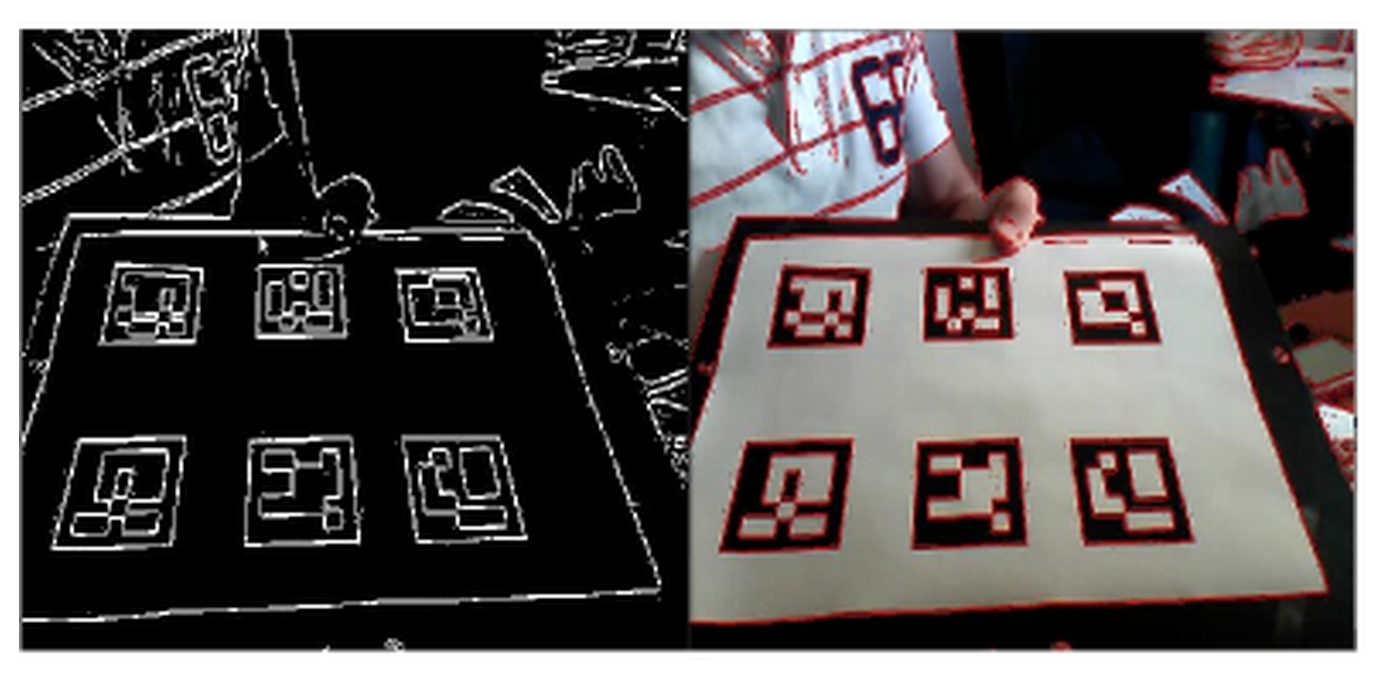
\includegraphics[scale=0.6, angle=0]{Files/Figures/aruco1.png}
    \caption[Παράδειγμα εντοπισμού marker και επαύξησης της σκηνής \cite{howmarkerswork}]{ Παράδειγμα εντοπισμού marker και επαύξησης της σκηνής }
    \label{fig:aruco1}
\end{figure}

\begin{figure}[H]
    \centering
    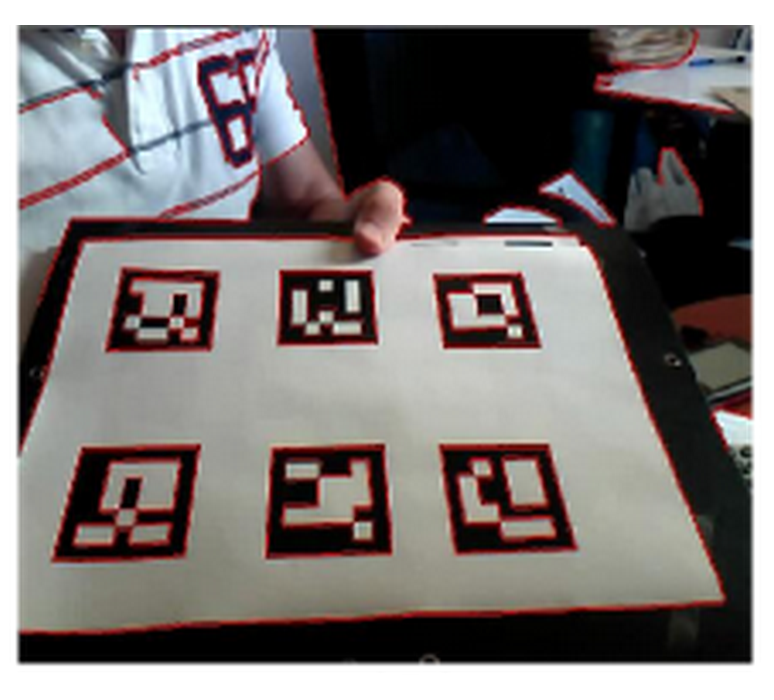
\includegraphics[scale=0.6, angle=0]{Files/Figures/aruco2.png}
    \caption[Παράδειγμα εντοπισμού marker και επαύξησης της σκηνής \cite{howmarkerswork}]{ Παράδειγμα εντοπισμού marker και επαύξησης της σκηνής \cite{howmarkerswork}}
    \label{fig:aruco2}
\end{figure}


\begin{figure}[H]
    \centering
    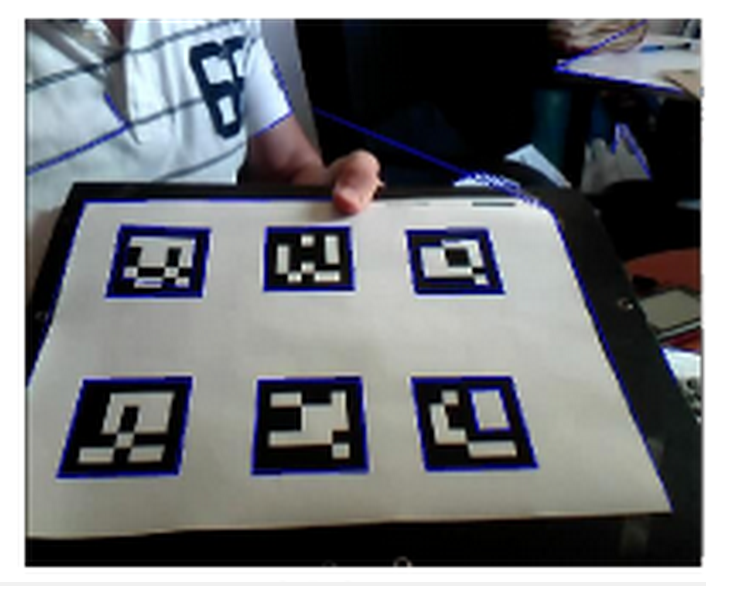
\includegraphics[scale=0.6, angle=0]{Files/Figures/aruco3.png}
    \caption[Παράδειγμα εντοπισμού marker και επαύξησης της σκηνής \cite{howmarkerswork}]{ Παράδειγμα εντοπισμού marker και επαύξησης της σκηνής \cite{howmarkerswork}}
    \label{fig:aruco3}
\end{figure}


\begin{figure}[H]
    \centering
    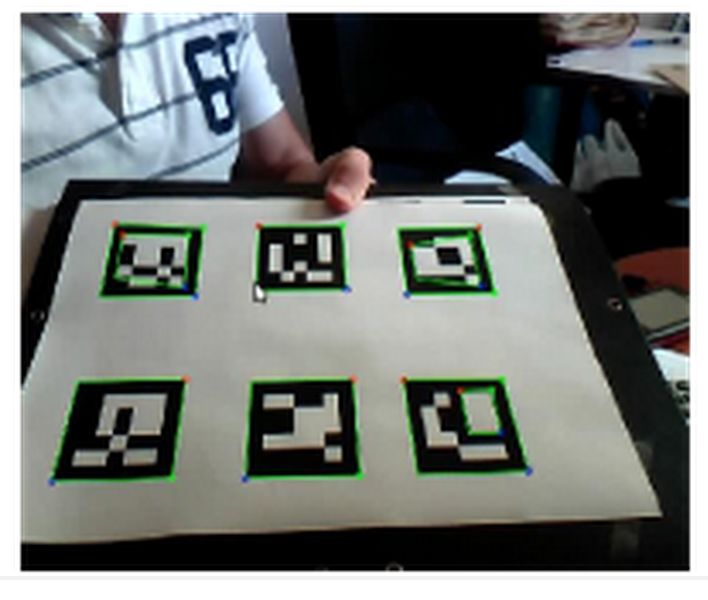
\includegraphics[scale=0.6, angle=0]{Files/Figures/aruco4.png}
    \caption[Παράδειγμα εντοπισμού marker και επαύξησης της σκηνής \cite{howmarkerswork}]{ Παράδειγμα εντοπισμού marker και επαύξησης της σκηνής \cite{howmarkerswork}}
    \label{fig:aruco4}
\end{figure}

\begin{figure}[H]
    \centering
    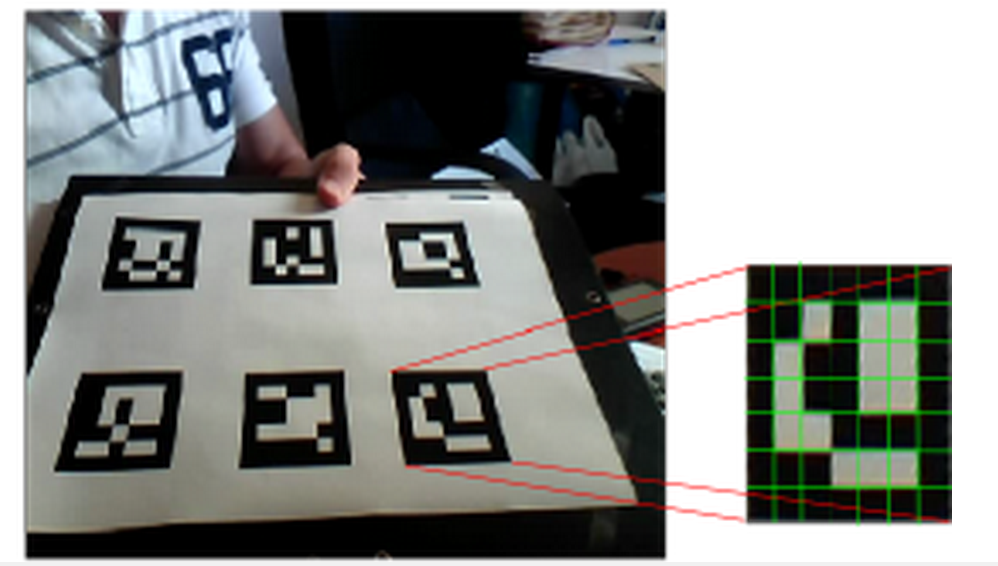
\includegraphics[scale=0.6, angle=0]{Files/Figures/aruco5.png}
    \caption[Παράδειγμα εντοπισμού marker και επαύξησης της σκηνής \cite{howmarkerswork}]{ Παράδειγμα εντοπισμού marker και επαύξησης της σκηνής \cite{howmarkerswork}}
    \label{fig:aruco5}
\end{figure}

\begin{figure}[H]
    \centering
    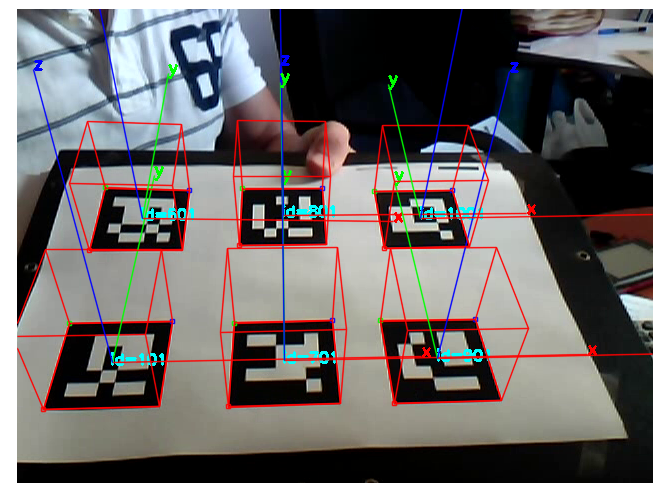
\includegraphics[scale=0.6, angle=0]{Files/Figures/aruco6.png}
    \caption[Παράδειγμα εντοπισμού marker και επαύξησης της σκηνής \cite{howmarkerswork}]{ Παράδειγμα εντοπισμού marker και επαύξησης της σκηνής \cite{howmarkerswork}}
    \label{fig:aruco5}
\end{figure}


\begin{figure}[H]
    \centering
    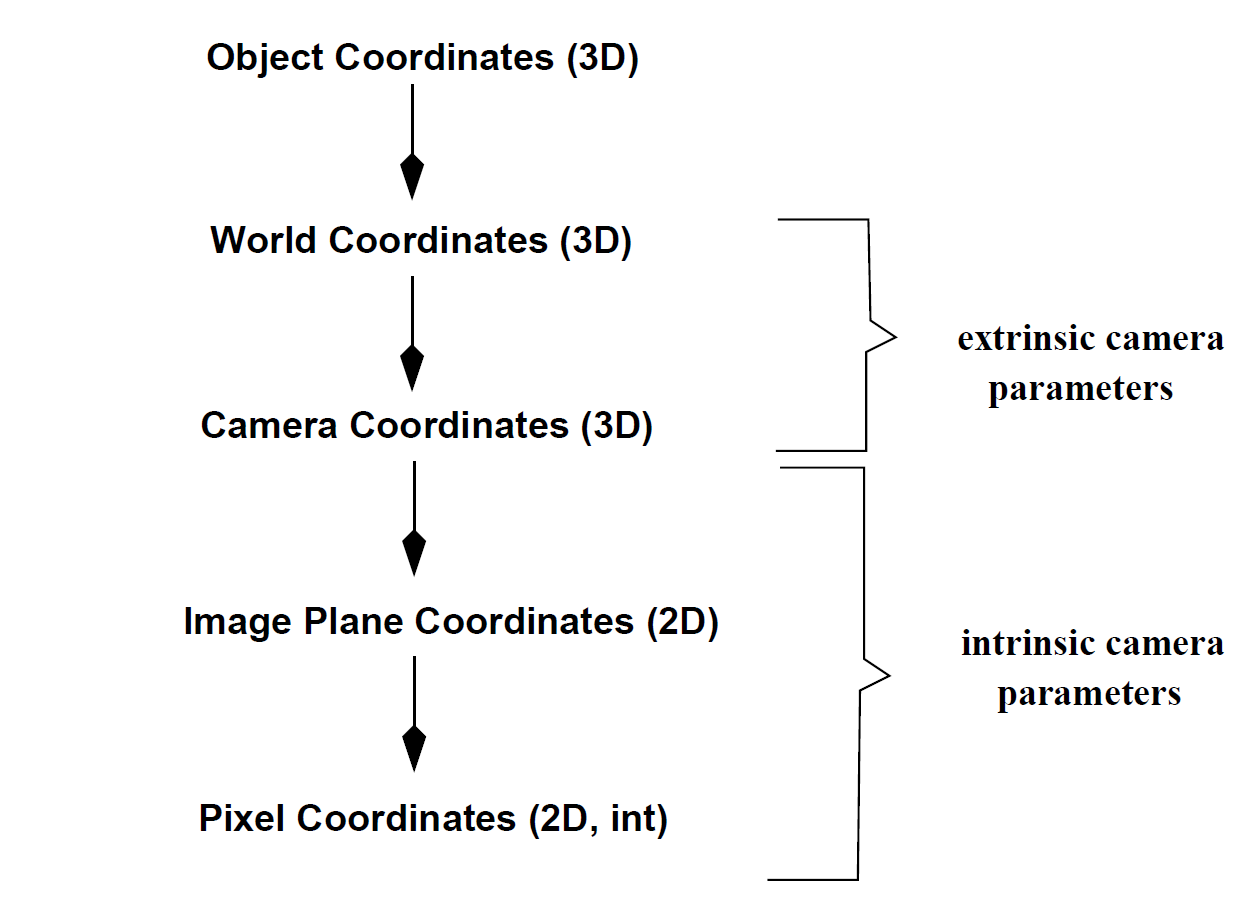
\includegraphics[scale=0.7, angle=0]{Files/Figures/coordinatesDiagram.png}
    \caption[Σειρά μετασχηματισμών]{ Σειρά μετασχηματισμών}
    \label{fig:coordinatesDiagram}
\end{figure}




\subsection{Εκτίμηση Θέσης Marker}



%malik
-συστήματα συντεταγμένων
Οι παρακάτω 3 μετασχηματισμοί όπως περιγράφονται στο \cite{Vallino1998}, που πρέπει να γίνουν γνωστοί πριν την ανάπτυξη εφαρμογών επαυξημένης πραγματικότητας είναι οι μετασχηματισμοί αντικειμένου-σε-κοσμικές, κοσμικές-σε-κάμερας, κάμερας-σε-επίπεδο εικόνας. 

\textbf{Object-to-World Transformations ($M_{O}$)}

Αν υποθέσουμε ότι έχουμε ένα εικονικό αντικείμενο κεντραρισμένο ως προς το τοπικό του σύστημα συντεταγμένων, το $M_{O}$ ορίζεται ως ο μετασχηματισμός από το τοπικό αυτό σύστημα σε μία θέση και έναν προσανατολισμό μέσα στο κοσμικό σύστημα συντεταγμένων που ορίζει την κύρια σκηνή.

\textbf{World-to-camera ($M_{c}$)}

Ο μετασχηματισμός $M_{c}$ ορίζει τη θέση και τον προσανατολισμό (πόζα) της βιντεοκάμερας που χρησιμοποιείται για τη θέαση της κύριας σκηνής, επιτρέποντας σε σημεία του πραγματικού κόσμου να οριστούν ως προς την κάμερα.

\textbf{Camera-to-image plane ($M_{p}$)}

Ο μετασχηματισμός $M_{p}$ ορίζει μία προβολής από το 3D χώρο στο 3D χώρο, έτσι ώστε οι συντεταγμένες της κάμερας να μπορούν να μετασχηματιστούν σε συντεταγμένες εικόνας, προκειμένου να μπορούν να προβληθούν σε μία οθόνη ή σε ένα HMD.


\begin{figure}[H]
    \centering
    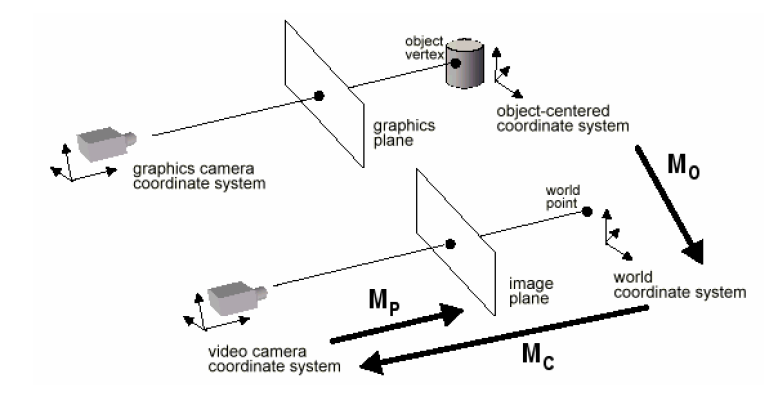
\includegraphics[scale=1.3, angle=0]{Files/Figures/coordinatesystems.png}
    \caption[Συστήματα Συντεταγμένων στην Επαυξημένη Πραγματικότητα]{Συστήματα Συντεταγμένων στην Επαυξημένη Πραγματικότητα}
    \label{fig:coordinatesystems}
\end{figure}

Για να μπορέσει μία εφαρμογή επαυξημένης πραγματικότητας να απεικονίσει σωστά ένα εικονικό τρισδιάστατο αντικείμενο πάνω από μία πραγματική σκηνή, οι παραπάνω γεωμετρικοί μετασχηματισμοί πρέπει να είναι ακριβείς.

Ένα σφάλμα σε οποιαδήποτε από τις σχέσεις θα κάνει ανακριβές το registration, reducing the realism of the final augmented scene.

Χρησιμοποιώντας ομογενή συστήματα συντεταγμένων, η προφανής ενός τρισδιάστατου σημείου στον Ευκλείδιο χώρο [x, y, z, w] χρησιμοποιώντας την παρακάτω εξίσωση:

\begin{equation}
\begin{bmatrix}
u & v & h
\end{bmatrix}
^{T}=
M_{P(3x4)}M_{C(4x4)}M_{O(4x4)}
\begin{bmatrix}
x & y & z & w
\end{bmatrix}
^{T}
\end{equation}

Οι παρακάτω ενότητες θα παρουσιάσουν έννοιες της προβολικής όρασης που θα μας βοηθήσουν να υπολογίσουμε τους μετασχηματισμούς 
$M_{P}$, $M_{C}$, και $M_{O}$.



%τζιονας
Η εύρεση των εξωτερικών παραμέτρων ( με δεδομένη την εκ των προτέρων γνώση των εσωτερικών παραμέτρων) που δίνουν τη θέση και τον προσανατολισμό της κάμερας σε σχέση με τον πραγματικό δισδιάστατο κόσμο είναι γνωστή σαν εκτίμηση πόζας (pose estimation).

H σημασία της στην επαυξημένη πραγματικότητα είναι τεράστια, ιδιαίτερα στην περίπτωση που είναι επιθυμητή η επικάθιση 3D γραφικών σε σε μία εικόνα-όψη του πραγματικού κόσμου. ρίσκοντας τη θέση και τον προσανατολισμό της πραγματικής κάμερας, μπορούμε να "ευθυγραμμίσουμε" με αυτή την εικονική κάμερα του αντίστοιχου τρισδιάστατου μοντέλου. Σαν απότελεσμα έχουμε την εμφάνιση της σωστής όψης του 3D μοντέλου, στο κατάλληλο μέγεθος και στο κατάλληλο μέρος.

Οι εξωτερικές παράμετροι της κάμερας που αναζητούνται κατά την pose estimation είναι 2 πίνακες:

\begin{itemize}
\item Ο πίνακας R (rotation), μεγέθους 3x3, που αποτελείται από 3 διανύσματα στοιχειωδών περιστροφών $R=\begin{bmatrix} R1 & R2 & R3 ] \end{bmatrix}$. Τα διανύσματα αυτά αντιπροσωπεύουν, όπως προαναφέρθηκε, την περιστροφή της κάμερας γύρω από τους 3 άξονες ενός συστήματος συντεταγμένων (3 βαθμοί ελευθερίας)
\item Ο πίνακας t μεγέθους 3x1, που αντιπροσωπεύει τη μετατόπιση της κάμερας. Κάθε στοιχείο του διανύσματος εκφράζει τη μετακίνηση στον κατάλληλο άξονα του συστήματος συντεταγμένων (3 βαθμοί ελευθερίας).
\end{itemize}

%εικονα

Συνοψίζοντας, κατά τη διαδικασία pose estimation ψάχνουμε να βρούμε 6 παραμέτρους συνολικά, γιαυτό γίνεται λόγος για pose estimation 6 βαθμών ελευθερίας.

Όπως μπορεί να γίνει εύκολα αντιληπτό, ο συνδυασμός αυτός της rotation και της translation μπορεί να μοντελοποιήσει οποιαδήποτε κίνηση της κάμερας.

%eikona

Η ανάλυση των μεθόδων pose estimation ξεφεύγει από τους στόχους της εργασίας, όμως θα παρουσιαστεί η μέθοδος που χρησιμοποιήθηκε.



\subsection{Multimarker Setup}




%from summary
Στις προηγούμενες ενότητες αναφερθήκαμε στις διαδικασίες, εκείνες, που είναι απαραίτητες για την ανίχνευση markers σε μία σκηνή με στόχο την εύρεση της σχετικής θέσης της κάμερας ως προς το marker. Ωστόσο ο εντοπισμός ενός marker μπορεί να αποτύχει για διάφορους λόγους όπως οι κακές συνθήκες φωτισμού της σκηνής, ορισμένες γρήγορες κινήσεις της κάμερας, αποκρύψεις του marker από άλλα αντικείμενα ή από τα χέρια του χρήστη κ.λ.π. 



Για να λυθεί αυτό το πρόβλημα, ορισμένες βιβλιοθήκες επιτρέπουν τη χρήση πολλαπλών markers μαζί τα οποία ονομάζονται πεδία markers ή markerboards. Ένα markerboard είναι ένας markers που αποτελείται από αρκετούς άλλους markers καθορισμένους σε μία διάταξη. Τα markerboards παρουσιάζουν δύο κύρια πλεονεκτήματα. 

Πρώτα απ'όλα έχουν περισσότερα από ένα markers, που σημαίνει ότι είναι δυσκολότερο να χαθούν όλα την ίδια στιμή. Επίσης όσο περισσότερα markers ανιχνευθούν, τόσο περισσότερα σημεία είναι διαθέσιμα για τον υπολογισμό των εξωτερικών παραμέτρων της κάμερας.
Επομένως, η ακρίβεια του συστήματος αυξάνεται. 


%siltanen
Οι 4 γωνίες ενός marker καθορίζουν την πόζα της κάμερας όπως αναφέρθηκε και προηγουμένως. Ωστόσο, η χρήση επιπλέον σημείων σταθεροποιεί το σύστημα tracking, βελτιώνοντας την ακρίβεια και επιτρέποντας στο σύστημα να αφαιρέσει ακραίες τιμές. Ειδικά αν υπάρχει θόρυβος, επιπλέον σημεία αναφοράς μπορούν να βελτιώσουν την ακρίβεια και την ανθεκτικότητα του συστήματος. Τρεις κύριες προσεγγίσεις που χρησιμοποιούνται για την ανίχνευση της πόζας είναι:

\begin{itemize}
\item Η χρήση περισσότερων από 4 σημείων ανά marker
\item Η χρήση περισσότερων από 1 markers
\item Η χρήση φυσικών χαρακτηριστικών σε συνδυασμό με markers.
\end{itemize}


Η βελτίωση στη σταθερότητα της πρώτης προσέγγισης είναι μικρή, καθώς τα σημεία κατανέμονται σε μία φυσικά στενή περιοχή και επομένως αυξάνουν τη σταθερότητα ελάχιστα. Ένα γνωστό πρόβλημα στο tracking είναι το γεγονός ότι το πεδίο όρασης των καμερών (field-of-view) είναι στενό ειδικά σε φορητές συσκευές. Αν ο χρήστης μετακινήσει την κάμερα, τότε χάνεται η θέα του marker. Ένα ευρύτερο field-of-view δε βοηθά ιδιαίτερα αν ο χρήστης περιστρέψει την κάμερα. Έπομένως η χρήση ενός συστήματος ανίχνευσης ενός marker περιορίζει τις επιτρεπτές κινήσεις του χρήστη, καθώς η κάμερα πρέπει να βλέπει το marker συνεχώς.

Αυτός ο περιορισμός δεν είναι επιθυμητός σε πολλές εφαρμογές και επομένως, η δεύτερη και η τρίτη επιλογή προτιμούνται. Τα συστήματα επαυξημένης πραγματικότητας τα χρησιμοποιούν για να βελτιώσουν την χρησιμότητα και τη ανθεκτικότητα ενός συστήματος.
Σε αυτή την ενότητα, αναφερόμαστε στη δεύτερη επιλογή και περιγράφουμε πως ένα σύστημα επαυξημένης πραγματικότητας μπορεί να ορίσει και να ανιχνεύσει ένα multi-marker setup. 

Ένα σύστημα ανίχνευσης μπορεί να ανταπεξέλθει σε μεγάλες κινήσεις της κάμερας, αν ο χρήστης κατανείμει αρκετούς markers σε διαφορετικές κατευθύνσεις. Όταν το σύστημα ανιχνεύσει και εντοπίσει κάθε marker ξεχωριστά, η πληροφορία που σχετίζεται με κάθε marker χάνεται, μόλις στο σύστημα είναι ανέφικτο να εντοπίσει το marker. 
Τα συστήματα Multi-marker ή αλλιώς πεδία markers, συνδυάζουν την πληροφορία από όλα τα markers και επομένως παρουσιάζουν μεγαλύτερη ακρίβεια.\cite{yoon2006increasing}. Για παράδειγμα, μπορούν να διαχειριστούν μερικές αποκρύψεις και να εξάγουν τη θέση ενός marker ακόμα και αν είναι αόρατο, αρκεί να γίνει η ανίχνευση άλλων markers που ανήκουν στο ίδιο πεδίο των markers. Ένα multi-marker setup είναι ένα σύστημα που χρησιμοποιεί πολλά markers μαζί, για την εκτίμηση της πόζας της κάμερας. Ένα σύστημα, όπου κάθε marker χρησιμοποιείται ξεχωριστά για τον υπολογισμό της σχετικής πόζας ως προς την κάμερα δεν θεωρείται multi-marker, ακόμα και αν χρησιμοποιηθούν αρκετοί marker.

Προκειμένου να εξάγουμε τη θέση ενός μη εντοπισμένου marker, ένα σύστημα πρέπει να ξέρει τη σχετική θέση ενός marker σε σχέση με τα άλλα. Είτε η σχετική θέση των markers πρέπει να είναι προκαθορισμένη, ή το σύστημα πρέπει να επιτρέψει την ελεύθερη κατανομή των markers και να εξάγει μία διάταξη δεικτών καθώς τα ανιχνεύει. 

Προκαθορισμένα συστήματα multi-marker χρησιμοποιούνται ευρέως και υποστηρίζονται από αρκετά εργαλεία και βιβλιοθήκες. Για παράδειγα, το ARToolKit \cite{artoolkit}, η ALVAR \cite{alvar} και η ArUco\cite{aruco} διαθέτουν υποστήριξη. Η προσέγγιση ενός setup με επίπεδο multi-marker, είναι ίδια με τη χρήση ενός μεγάλου marker με περισσότερα από 4 σημεία. Τώρα το πεδίο των markers είναι ένα μεγάλο marker και τα markers μέσα σε αυτό είναι υπο-χαρακτηριστικά. 

Ένα σύστημα multi-marker μπορεί να χρησιμοποιήσει ένα ανεπίπεδο προκαθορισμένο marker επίσης, για παράδειγμα οι marker μπορούν να καλύπτουν τις πλευρές ενός κύβου, ορισμένοι να είναι σε ένα τοίχο κλπ.\cite{uematsu2005ar}
Οι προσεγγίσεις αυτές παρέχουν πληροφορίες ανίχνευσης για περιβάλλοντα μεγαλύτερης κλίμακας από συστήματα ανίχνευσης ενός μόνο marker. 

Τα markers τα οποία επισυνάπτονται πάνω σε τρισδιάστατα αντικείμενα επιτρέπουν στο σύστημα να τα ανγνωρίσει από διαφορετικές οπτικές γωνίες, κάτι το οποίο είναι επιθυμητό με tangible διεπαφές.
Το πρόβλημα με τις ανεπίπεδες προσεγγίσεις έχει να κάνει με το γεγονός ότι είναι δύσκολο να μετρηθεί η φυσική θέση και ο προσανατολισμός κάθε marker σε σχέση με ένα άλλο.
Αυτή η διαδικασία βαθμονόμησης απαιτεί χρόνο και είναι ανακριβής αν γίνει χειροκίνητα. [8]. Μπορούν να χρησιμοποιηθούν εξωτερικές βοήθειες για τη μέτρηση των θέσεων των markers, όπως για παράδειγμα ένα ταχόμετρο, αλλά οι οπτικές προσεγγίσεις έχουν μεγαλύτερο ενδιαφέρον από τη σκοπιά ενός συστήματος επαυξημένης πραγματικότητας αφού ένα τέτοιο σύστημα περιλαμβάνει μία κάμερα και μία υπολογιστική μονάδα έτσι και αλλιώς.

Κατά την δημιουργία ενός multi-marker setup, ο χρήστης μπορεί να τοποθετήσεις markers ελεύθερα σε ένα χώρο χωρίς προκαθορισμένους περιορισμούς και έπειτα το σύστημα δημιουργεί το πεδίο των markers με βάση την παρατήρηση των θέσεων των markers.

Η διαδικασία αυτή καλείται αυτόματη ανακατασκευή multi-marker setups.






\section{Αναγνώριση Χειρονομιών}
%ΓΕΝΙΚΑ ΓΙΑ ΤΗΝ ΑΝΑΓΝΩΡΙΣΗ ΧΕΙΡΟΝΟΜΙΩΝ ΚΑΙ ΤΗΝ ΚΟΙΝΩΝΙΚΗ ΑΠΟΔΟΧΗ ΚΑΙ ΤΗ ΧΡΗΣΙΜΟΤΗΤΑ ΣΕ ΕΦΑΡΜΟΓΕΣ


%Από εργασία μου δερματά

H αναγνώριση χειρονομιών είναι η διαδικασία κατά την οποία οι χειρονομίες οι οποίες γίνονται από τον χρήστη αναγνωρίζονται από έναν δέκτη. Η αναγνώριση και η ερμηνεία των χειρονομιών απαιτεί από μία μηχανή την ικανότητα να μετρήσει τις δυναμικές ή στατικές παραμορφώσεις του χεριού, του βραχίονα ή ακόμα και άλλων μερών του ανθρωπίνου σώματος, τα οποία συμμετέχουν στην κίνηση.

Σε κάθε σύστημα αναγνώρισης χειρονομιών το πρώτο στάδιο είναι η συλλογή δεδομένων από τον χρήστη.Οι πρώτες συσκευές συλλογής δεδομένων βασιζόντουσαν στη χρήση data gloves και καλωδίων, πράγμα που εμπόδιζε την φυσικότητα στην αλληλεπίδραση του χρήστη.Οι σημερινές προσεγγίσεις αξιοποιούν την χρήση βιντεοκάμερων και τεχνικών υπολογιστικής όρασης που καταγράφουν το αντικείμενο και με τεχνικές αναγνώρισης αναλύουν και ερμηνεύουν τις χειρονομίες.

Πολλές και ποικίλες είναι οι προσεγγίσεις των ερευνητών στην αναγνώριση των χειρονομιών.Αυτά που διαφέρουν σε κάθε προσέγγιση είναι ο τρόπος με τον οποίο κάθε ερευνητής κατάφερε να συλλέξει δεδομένα και οι τεχνικές επεξεργασίας εικόνας που εφάρμοσε για να εξάγει χαρακτηριστικά.

Οι νοηματικές χειρονομίες μπορούν να είναι πολύ σύνθετες, περιέχοντας ταυτόχρονες κινήσεις διάφορων σημείων, ωστόσο πρέπει να περιγραφούν στον υπολογιστή με τρόπο απλό και σαφή.

%hoggan
Οι χειρονομίες χρησιμοποιούνται ως μέσο αλληλεπίδρασης σε πολλά διαφορετικά είδη συσκευών και εφαρμογών. Μία από τις πιο γνωστές χειρονομίες είναι αυτή της χειρονομίας του "τσιμπήματος", που περιλαμβάνει την διαστολή ή συστολή της έκτασης των δακτύλων \cite{hoggan2013multi}.


Pinch It is defined as the movement of expansion and contraction of a nger spread. It has been used for different purposes depending on target applications, e.g. the zooming metaphor by contracting and expanding, scaling or picking. It resembles a grabbing or picking action and offers natural signal to select or move an object in an interactive system and due to the nature of the thumb and index ngers, the pinch grabbing is precise and has high performance.


Human interaction with computer technology has for many years been a machine-centric form of communication. It has relied on the user’s ability to conform to interface strategies that better suit the technology than the user. As the use of computer technology spreads, the physical and expressive limitations of current interaction methods are increasingly counter-productive. Current interface technology such as the mouse and keyboard associated with desktop computers has become ubiquitous in mainstream computing. This role is based on application interface technology that has been used for decades. As the application domain expands, this technology will reveal its performance inhibitions. In an effort to overcome the barrier associated with current interface solutions, much research is being done in the domain of gesture recognition. Because gesture recognition is a natural form of human expression, it seems reasonable to apply it to the communication channel of Human-Computer Interaction (HCI). Several techniques for capturing gesture have been proposed [OKA02, ULHA01, CROW95]. Gesture interpretation for HCI requires the measurability of hand, arm and body configurations. Initial methods were attempted to directly measure hand movements using glove-based strategies. These methods required that the user be attached to the computer through the connecting cables. This restricts the user significantly in their environment.

Overcoming this contact-based interpretation requires the inference-based methods of computer vision. As processor power continues to rise, the once complex algorithms of the field are becoming available as real-time applications. Most computer vision-based gesture recognition strategies focus on static hand gestures known as postures. However, it has been argued that the motion within gesture communication conveys as much meaning as the postures themselves. Examples include global hand motion and isolated fingertip motion analysis. The interpretation of gesture can be broken down into three phases: modeling, analysis and recognition. Gesture modeling involves the schematic description of a gesture system that accounts for its known or inferred properties. Gesture analysis involves the computation of the model parameters based on detected image features captured by the camera. The recognition phase involves the classification of gestures based on the computed model parameters. These phases are outlined in figure 2.12.

Although much research has been done in the field of gesture recognition, HCI interaction involving accurate, real-time interpretation is a long way off. The key to simplifying the domain of human gesture possibilities is to construct a gesture model which clearly describes the sub-domain of gesture that will be classified by the associated system.



To determine an appropriate model for a given HCI system, the application must be clearly defined. Simple gesture requirements result in simple gesture models. Likewise, complex gesture interpretation, involves defining a complex model.

Gesture is defined as the use of body and motion as a form of expression and social interaction. This interaction must be interpreted for communication to be successful. Gesture interpretation is considered a psychological issue, which plays a role in the taxonomy of the varying types of human gesture. Figure 2.13 outlines one such taxonomy.

It is crucial for any gesture recognition system to distinguish between the higher level classifications such as gesture versus unintentional movements and manipulation versus communicative. It has been suggested that the temporal domain of human gesture, for example, can help classify a gesture from unintentional movement. The temporal aspect of gesture has three phases: preparation, nucleus, and retraction [PAVL97]. The preparation phase involves the preparatory movement of the body from its rest position. The nucleus phase involves a definite form of body, while the retraction phase describes the return of the body to its rest position. The preparation and retraction phase are characterized by rapid motion, whereas the nucleus phase shows relatively slow motion. Some measurable stray from these temporal properties could indicate unintentional movement as opposed to gestures in the classification process. Two forms of modeling are being explored; appearance and 3D model-based modeling. Appearance-based modeling deals with the direct interpretation of gesture from images using templates. Image content features such as contours, edges, moments and even fingertips can form a basis for parameter extraction with respect to the gesture model chosen. Three-dimensional model-based modeling is used to describe motion and posture in order to then infer the gesture information. Volumetric models are visually descriptive, but are complex to interpret using computer vision. Skeletal models describe joint angles which can be used to infer posture and track motion.


\subsection{Αναγνώριση Blob}
%ΤΙ ΕΙΝΑΙ Η ΑΝΑΓΝΩΡΙΣΗ BLOB


\subsection{Αναγνώριση Χειρονομίας Τσιμπήματος}
%ANALYΣΕ ΤΟ PINCH, ΠΩΣ ΓΙΝΕΤΑΙ, ΓΙΑΤΙ ΕΙΝΑΙ ΕΥΚΟΛΟ,ΠΟΥ ΧΡΗΣΙΜΟΠΟΙΕΙΤΑΙ, ΠΩΣ ΑΝΙΧΝΕΥΕΤΑΙ(WILSON,ETC)

%wang-popovi


Pinching has been shown to be an effective gesture for “clicking”
in 3D space. Hilliges and colleagues use a single depth
camera to detect pinches above a table top [9]. Benko and
Wilson [4] track pinches using an infrared camera above a
projector. Wilson uses a webcam to detect pinches above
the keyboard [26]. However, all three approaches rely on
a single-view pinch detection technique that suffers from occlusions,
restricting the hand orientations that can be tracked.
A unique feature of our approach is the use of two widebaseline
viewpoints. Our two-view approach resolves occlusions
from one view using information from the other, enabling
robust gesture (e.g. pinch) detection. Our contribution
is independent of the particular type of camera used (depth
or RGB).
%--

Successful gesture recognition requires clear classification of the model parameters. This process can be difficult when attempting feature extraction schemes that rely on complex computer vision techniques. For example, contours can be misinterpreted when used for the recognition of gesture so their use is usually restricted to tracking. On the other hand, slight changes in hand rotation while presenting the same posture can be interpreted as different postures using geometric moments. Temporal variance is an important issue that needs to be studied in more detail. For example, hand clapping should be recognized properly regardless if it is done slowly or quickly. Hidden Markov Models (HMMs) have shown promise in distinguishing gesture in the presence of duration and variation changes

Another recognition approach is to use motion history images (MHIs) or temporal templates. Motion templates accumulate the motion history of a sequence of visual images into a single two-dimensional image. Each MHI is parameterized by the time history window that was used for its computation. Multiple templates with varying history window times are gathered to allow time duration invariance. This process is computationally simple, but recognition problems can stem from the presence of artifacts in the images when auxiliary motions are present. Although it seems that 3D model-based approaches can capture the richest set of hand gestures in HCI, the applications that use such methods are rarely real-time. The most widely used gesture recognition approaches use appearance-based models. Current applications in the field of hand gesture related to HCI are attempting to replace the keyboard and mouse hardware with gesture recognition. Exciting possibilities with helping physically-challenged individuals and the manipulation of virtual objects are being explored.



%\section{Διαδραστική Επαυξημένη Πραγματικότητα}
%OTI ΔΕΝ ΕΙΠΑΜΕ ΣΤΗΝ ΕΙΣΑΓΩΓΗ ΓΙΑ AR, ΚΥΡΙΩΣ ΑΝΑΦΟΡΑ ΕΡΓΑΣΙΩΝ ΠΟΥ ΑΣΧΟΛΟΥΝΤΑΙ ΜΕ INTERACTION OF VIRTUAL OBJECTS, KAI MEΘΟΔΟΥΣ ΠΟΥ ΧΡΗΣΙΜΟΠΟΙΟΥΝΤΑΙ, ΓΙΑΤΙ ΕΙΝΑΙ ΧΡΗΣΙΜΗ Η ΑΛΛΗΛΕΠΙΔΡΑΣΗ ΣΤΟ ar


\section{Σχετικές Ερευνητικές Εργασίες}
%ΑΝΑΦΕΡΕ ΠΑΡΟΜΟΙΕΣ ΕΡΓΑΣΙΕΣ ΓΙΑ GESTURE INTERACTION, AR TABLETOP GAMING, KAI AZUMA CLASSICS ETC.
%ΠΕΣ ΣΙΓΟΥΡΑ ΓΙΑ ΠΑΡΟΜΟΙΑ ΣΚΑΚΙΑ ΣΤΟ ΤΕΛΟΣ
%ΨΑΧΝΟΝΤΑΣ ΣΕ PAPERS ΑΝΑΦΕΡΕ ΠΑΡΟΜΟΙΕΣ ΕΡΓΑΣΙΕΣ ΝΑ ΕΧΟΥΝ ΣΧΕΣΗ ΜΕ GESTURE RECOGNITION FOR AR, VIRTUAL OBJECT MANIPULATION, AR TABLETOP GAMES
Σε προηγούμενες ερευνητικές εργασίες, παρουσιάστηκαν διαφορετικές προσεγγίσεις για την κατανόηση των δυνατοτήτων που προσφέρουν οι χειρονομίες στην αλληλεπίδραση με εικονικά αντικείμενα σε ένα περιβάλλον επαυξημένης πραγματικότητας. Επιπλέον, σε βιβλιογραφικές αναφορές μπορούμε να εντοπίσουμε τις δυνατότητες της επαυξημένης πραγματικότητας στον χώρο της ψυχαγωγίας και συγκεκριμένα των βιντεοπαιχνιδιών, τις βασικές έννοιες της αλληλεπίδρασης μεσω χειρονομιών και της ρεαλιστικής απεικόνισης εικονικών αντικειμένων.


%thomas-cie-apps of ar gaming
Augmented reality chess games have been implemented on previous works. One approach
[1] used a handheld pen prop with a marker cube on top of it in order to interact with the
chess pieces. As the writers admit, the tracking of interaction props was inaccurate and slow
to provide unencumbered and natural use. Another one[2] used nger tracking techniques that
allow gestural interaction with the chess pieces. In this approach, manipulation of virtual objects
is possible using grab and release gestures, as well as image processing techniques to detect hand
gestures, using a single camera. The nger tracker that is implemented is using a hands 3D
model that can determine enough information to robustly track the position, orientation and
pose of the users index nger. However, this solution resorts to using a marked glove with
retro-re
ective spheres on top of the forengers joints, something that may disturb users and is
denitely not a natural way to interact with content. Other approaches utilize mobile markers
that correspond to a specic type of chess piece and users had to move the markers to different
positions of a chessboard in order to play the chess game. Of course this would take quite an
amount of effort to correctly print and create the congurable chessboard and is really similar
to just using a real chessboard with real chess pieces.


Η εφαρμογή AR2Hockey ήταν ένα από τα πρώτα βιντεοπαιχνίδια στο χώρο της επαυξημένης πραγματικότητας[Ohshima et al. 1998]. Στο συγκεκριμένο παιχνίδια, χρησιμοποιοιείται τεχνολογία optical see-through HMD display για 2 παίκτες. The game is played on a standard table with landmarks. The landmarks allow for a hybrid optical tracking and the Polhemus’ Fastrack. The game basically supports the traditional form of air hockey, but replaces the physical pucks with virtual ones. As an extension to this,Mueller et al. developed an AR remote version of air hockey [Mueller et al. 2006]. Two remote physical air hockey tables, one for each player, provide the playing surface for the game. There is a video conferencing display across the middle of each table providing a real-time video feed of the other player. What makes this game different is that the users play with physical pucks. Once a puck is hit across the table, it is caught with a mechanism under the video conference display. The mechanism then automatically shoots the puck back in response to the shot from the other player. The game of pool (or billiards) has been investigated by a number of researchers as an application domain for AR. Jebara et al. developed the first mobile AR pool system [Jebara et al. 1997]. This is an HMDbased AR game, for which many of the first algorithms for image processing and physics engines for pool-based games were developed. This game served as a trainer for the end user by displaying AR information on the correct cue placement. Each of these games supports a physical gaming interface, adding to the evidence that AR incorporates both the physical and virtual worlds. AR2Hockey was a very early AR game, and as such required more expensive display and tracking equipment; but the price for both these forms of hardware has fallen dramatically. The Jebara et al. pool system also required a large structure, the pool table, to play the game upon. This system also incorporates a tutoring system for the players, including suggestions for shots.


A number of AR card games have been developed: Billinghurst et al. created an ARToolkit memory game, where the users flip physical cards [Billinghurst et al. 2000]. When a card is flipped over, a 3D graphic is displayed. The cards interact with each other by playing an animation when there is a match between the cards. This was the first AR game developed with the ARToolkit. Diaz et al. created a variant which employed hand gestures as the means of interaction [Diaz et al. 2006]. They used special cards to enable the system to sense card flipping by embedding Hall effect switches in the cards. BattleBoard is another example of a tabletop AR card game [Andersen et al. 2004]. This is an ARToolkit fiducial marker-based AR system which attaches virtual game pieces to the markers. One player employs an HMD with a camera and the second player views the game through a monitor. Battles are fought when pieces come in close proximity to each other, and thus activate AR animations. The Billinghurst et al. card game was designed for a public demonstration at an ACM SIGGraph conference with quick gameplay. BattleBoard employs a similar technology to the Billinghurst et al. card game, but BattleBoard’s design is more advanced, and is similar to a duelling card game. The Tankwar game was developed for more extended gameplay, investigating how AR could be employed for games with a more traditional time span.


%interaction in ar games
A drama-based game, Fac¸ade, was extended into an HMD AR version, AR Fac¸ade [Dow et al. 2007a, 2006, 2007b]. This game is a major break from traditional AR gaming ideas developed previously. This is a complex, real-life, role-playing game; very much like interactive theatre. Originally, the game was played on a traditional workstation; AR Fac¸ade is played on a HMD with a mobile backpack system, with gestures and voice as the main forms of interaction. The authors constructed virtual and physical representations of many of the game objects, such as walls and furniture, in an apartment. Objects that were manipulated by both the virtual characters and the physical players were presented as AR objects to the game player in the HMD. Due to the large area the game is played in a large area with an IS1200 tracking system. A Wizard of Oz method was employed to support user interactions to make formore robust gesture and speech processing systems during user studies. The authors found this form of interaction engaging for the user, but more research is required

%playstation app with board and monitor for AR
Το βιντεοπαιχνίδι Eye of Judgement της πλατφόρμας Sony PS3 είναι ένα βιντεοπαιχνίδι επαυξημένης πραγματικότητας σε τρίτο πρόσωπο, που περιλαμβάνει μία ψηφιακή βιντεοκάμερα η οποία καταγράφει το ταμπλό του παιχνιδιού και απεικονίζει μία επαυξημένη του έκδοση στην τηλεόραση. Αυτός ο τύπος παιχνιδιού απαιτεί από τους χρήστες να επικεντρώνουν την προσοχή τους τόσο στο πραγματικό ταμπλό, όσο και στην έκδοση που παρουσιάζεται στην οθόνη. Μόλις οι κάρτες του παιχνιδιού τοποθετηθούν πάνω στο ταμπλό, δρουν ως καθοδηγητικοί δείκτες(markers) για τον εντοπισμό τεράτων επαυξημένης πραγματικότητας και τα κομμάτια του παιχνιδιού απεικονίζονται επάνω τους. Η μηχανή παιχνιδιών αναλαμβάνει τα τρισδιάστατα γραφικά των καρτών μόλις εντοπιστούν. Το παιχνιδί αυτό, ήταν ένα από τα πρώτα εμπορικά βιντεοπαιχνίδια επαυξημένης πραγματικότητας που κυκλοφόρησαν στην αγορά που επέτρεπε τη χρήση καθογητητικών δεικτών (fiducial markers).


%Εργασίες με σκάκι ή pinch gestures για χειρισμό εικονικών αντικειμένων 
Οι Dorfmuller-Ulhaas και Schmalstieg δημιούργησαν ένα σύστημα οπτικής ανίχνευσης δακτύλων, με απώτερο σκοπό την αφαίρεση των ενοχλητικών καλωδίων κατά τη διάρκεια της αλληλεπίδρασης με τα εικονικά αντικείμενα. Μάλιστα, η τεχνολογίας που ανέπτυξαν, παρουσιάστηκε μέσα από μία επαυξημένη έκδοση ενός πολύ γνωστού παιχνιδιού, που δεν είναι άλλο από το σκάκι. [Dorfmuller-Ulhaas and Schmalstieg 2001].

%vale kai mobile collaborative ar chess


%wang,popovi
RELATED WORK
Many methods have been proposed for markerless or gloveless
hand tracking, but they are either too slow for interactive
applications, e.g. [24, 7], or the range of poses that they can
detect do not permit the precise selection required in CAD
applications, e.g. [14, 13, 20]. In comparison, our system
achieves bimanual 6-DOF pose estimation at interactive rates
and reliably detects poses suited for discrete selection such as
pinching and pointing.
Glove tracking has been proposed to ease and speed up the
problem of hand tracking, e.g. [27, 25]. However, gloves are
a significant drawback if one wants to also use the keyboard
and mouse. Users may be reluctant to put on a glove when
switching from a 2D task such as menu navigation to a 3D
task such as object assembly. Wearing a glove may also become
uncomfortable during long work sessions.


%krevelen
Besides registering virtual data with the user‟s real world
perception, the system needs to provide some kind of interface
with both virtual and real objects. Our technological
advancing society needs new ways of interfacing with both
the physical and digital world to enable people to engage in
those environments [67]. 
WIMP (windows, icons, menus, and pointing), as the
conventional desktop UI metaphor is referred to, does not
apply that well to AR systems. Not only is interaction required
with six degrees of freedom (6DOF) rather than 2D, the use of conventional devices like a mouse and keyboard
are cumbersome to wear and reduce the AR experience.
Like in WIMP UIs, AR interfaces have to support selecting,
positioning, and rotating of virtual objects, drawing
paths or trajectories, assigning quantitative values (quantification)
and text input. However as a general UI principle,
AR interaction also includes the selection, annotation, and,
possibly, direct manipulation of physical objects. This
computing paradigm is still a challenge [20].




In stead of using hand-worn trackers, hand movement may
also be tracked visually, leaving the hands unencumbered. A
head-worn or collar-mounted camera pointed at the user‟s
hands can be used for gesture recognition. Through gesture
recognition, an AR could automatically draw up reports of
activities [105]. For 3D interaction, UbiHand uses
wrist-mounted cameras enable gesture recognition [14],
while the Mobile Augmented Reality Interface Sign Interpretation Language 16 [16] recognises hand gestures on a
virtual keyboard displayed on the user‟s hand (Fig. 12). A
simple hand gesture using the Handy AR system can also be
used for the initialization of markerless tracking, which estimates
a camera pose from a user‟s outstretched hand [97].
Cameras are also useful to record and document the user‟s
view, e.g. for providing a live video feed for teleconferencing,
for informing a remote expert about the findings of AR
field-workers, or simply for documenting and storing everything
that is taking place in front of the mobile AR system
user.
Common in indoor virtual or augmented environments is
the use of additional orientation and position trackers to
provide 6DOF hand tracking for manipulating virtual objects.
For outdoor environments, Foxlin and Harrington [60] experimented
with ultrasonic tracking of finger-worn acoustic
emitters using three head-worn microphones




Immersed in an environment containing virtual information, the user is left with few mechanisms for interacting with the virtual augmentations. The use of hardware devices [VEIG02] can be physically restrictive given the special freedom goals of Augmented Reality. Interaction with virtual augmentation through a physical mediator such as a touch screen [ULHA01] is becoming a common practice. An interesting alternative is the use of natural human gestures to communicate directly with the environment. Gesture recognition has been explored mainly for the purpose of communicative interaction. Gesture systems have explored many aspects of hand gesture including three-dimensional hand posture [HEAP96] and fingertip motion [OKA02, ULHA01, CROW95]. The system presented in this chapter attempts to bridge these two fields of study by describing a hand gesture system that is used for manipulative interaction with the virtual augmentation. Although natural human gestures are too complex to recognize in realtime, simple gesture models can be defined to allow a practical interactive medium for real-time Augmented Reality systems.


%vale to google glass manipulation project

\section{Προκλήσεις και Προβλήματα}
%ΣΥΓΧΡΟΝΑ ΠΡΟΒΛΗΜΑΤΑ ΣΤΟ AR

%ziegler
State of the Art Recent tracking systems produced very good results for indoor applications. Predominantly, they use hybrid approaches and work within a limited range (cp. [ZDB08, HF04, ABB+01]). According to Zhou et al.[ZDB08] current tracking systems consist of two stages. The first stage is dedicated to either learning and training or feature extraction. The second stage takes care of the tracking itself, using the knowledge gained through training or the features that have been extracted. The first stage usually requires the most computational resources, if the system uses a learning algorithm. Using a learning stage can reduce the resources the on-line tracking needs, enabling the system to work in real time. 2.3.5.1 Limitations and Challenges Even though tracking systems are accurate enough to achieve good results, the environments they work in are usually restricted not only to being indoors but also to being known in advance[ABB+01]. Dynamical adaption to unknown environments still poses a challenge. Complex scenes are challenging for real-time 3D tracking as is the motion of target objects[ZDB08]. Coping with rapid camera movements is difficult as resulting motion-blur hinders the re-observation of features. Rapid and unpredictable changes, that may occur in outdoor environments, constrain tracking results[HF04]. Especially illumination changes, which often and repeatedly occur outdoors, complicate the tracking process[ZDB08]. Basically all changes which cannot be controlled or anticipated are hard to handle. Some systems feature automatic reinitialisation, but the recovery of the camera pose, when the tracking has failed, cannot be achieved easily[ZDB08]. It is limited to applications which possess enough knowledge about the environment or which do not solely rely on vision-based tracking. 2.3.5.2 Trends Current research features many tracking approaches. Coping with unknown outdoor environments is an important topic. One way researchers are trying to achieve that is by further investigating hybrid approaches. As the growing number of publications during the past years indicate, Mobile AR becomes more and more popular among researches[SW07, WRM+08]. The growing computational resources of mobile devices present novel possibilities. The number of commercial applications from which users can choose continually rises. Among them are Layar9, Nokia Point \& Find10, Twitter AR11 and Virus Killer 36012. Building a reference presentation of the environment while tracking is a popular trend, research focusing especially on Simultaneous Localisation and Mapping (SLAM)[CGKM07, DRMS07, KM09]. Such systems usually require a high amount of computational resources. However, through certain restrictions, SLAM works on a mobile phone, too, as has recently been shown by the work of Klein and Murray[KM09]. Instead of using as many features as possible and hoping that some of the chosen features provide robust tracking, researchers try to find methods to detect only suitable and useful features in the first place[ZDB08, ST94]. Researchers try to find ways of making initialisation processes automatic[SKSK07]. Focusing on model-based tracking is popular as well[FL07, WS07]. Last but not least, ubiquitous tracking, that is tracking acquired by forming a dense network of sensors that enables tracking everywhere, seems to be achievable in the near future[HPK+07].


%--
Μία από τις μεγαλύτερες προκλήσεις με τις οποίες έρχονται αντιμέτωποι οι δημιουργοί εφαρμογών επαυξημένης πραγματικότητας είναι η σωστή τοποθέτηση του εικονικού αντικειμένου εντός του πραγματικού περιβάλλοντος, έτσι ώστε η συνθετική πληροφορία να δίνει την εντύπωση ότι ανήκει σε αυτό. Η διαδικασία αυτή είναι γνωστή ως registration (γεωαναφορά). Η σωστή συγχώνευση και ευθυγράμμιση των δύο κόσμων – του φυσικού και του παραγόμενου από υπολογιστή – είναι κύρια προϋπόθεση για την εκπλήρωση του στόχου των εφαρμογών επαυξημένης πραγματικότητας, ενώ λάθη ή ανακρίβειες στην τοποθέτηση του εικονικού αντικειμένου θα έχουν ως αποτέλεσμα να χαθεί η ψευδαίσθηση ότι οι δύο κόσμοι συνυπάρχουν [3]. Πολλές εφαρμογές, μάλιστα, όπως για παράδειγμα στην ιατρική, απαιτούν ακριβή γεωαναφορά και δεν είναι επιτρεπτά λάθη και αστοχίες. Για τη σωστή γεωαναφορά, απαραίτητη προϋπόθεση είναι η πρότερη ανίχνευση της θέσης και του προσανατολισμού της κάμερας – και γενικά της συσκευής μέσω της οποίας επαυξάνεται η πραγματικότητα – ή του κεφαλιού του χρήστη (π.χ. σε εφαρμογή με HMD). Η διαδικασία αυτή είναι γνωστή ως tracking (ανίχνευση), απαντά στα ερωτήματα: πού βρίσκεται ο χρήστης, πού εστιάζεται το ενδιαφέρον του και πού πρέπει να παρουσιαστεί το εικονικό αντικείμενο [72] και συνεπώς η σωστή και ακριβής, ανάλογα με την εφαρμογή διεκπεραίωσή της είναι κρίσιμη για τη δημιουργία πειστικών εφαρμογών επαυξημένης πραγματικότητας. Για την επίτευξη των τελευταίων, η ανίχνευση πρέπει πρακτικά να διεξάγεται σε πραγματικό χρόνο, δηλαδή η εκτίμηση της θέσης να γίνεται σε χιλιοστά του δευτερολέπτου, καθώς επίσης και να είναι εύρωστη, δηλαδή να δίνει ικανοποιητικά αποτελέσματα κάτω από ποικίλες συνθήκες, όπως για παράδειγμα σε μεταβαλλόμενο φωτισμό [68]. Υπάρχουν πολλές μέθοδοι ανίχνευσης 6 βαθμών ελευθερίας (6DOF tracking), όπως το μηχανικό tracking, τεχνική που υιοθετήθηκε και από το πρώτο σύστημα επαυξημένης πραγματικότητας του Sutherland, το υπερηχητικό tracking και το οπτικό tracking. Υπάρχουν και άλλες που υπολογίζουν μόνο θέση ή προσανατολισμό, όπως για παράδειγμα το tracking που βασίζεται σε πληροφορίες μόνο από GPS ή μόνο από γυροσκόπια [15]. Για εφαρμογές που απαιτούν ακριβή γεωαναφορά, ωστόσο, απαιτείται ακριβές στιγμιαίο 6DOF tracking υπό οποιεσδήποτε συνθήκες. Επειδή η τέλεια ανίχνευση είναι – τουλάχιστον προς το παρόν – ανέφικτη, εξαιτίας των χρονικών καθυστερήσεων ή και των περιορισμών λόγω ακριβείας, κύρια πρόκληση αποτελεί η εύρεση της μεθόδου ανίχνευσης που είναι ιδανική για τη συγκεκριμένη κάθε φορά εφαρμογή [73]. Υπάρχει ένας ακόμη αριθμός προκλήσεων που συνδέονται με το πρόβλημα της ανίχνευσης και τοποθέτησης του εικονικού αντικειμένου εντός του φυσικού περιβάλλοντος [4], η κυριότερη από τις οποίες είναι οι αποκρύψεις (occlusion). Σύμφωνα με την τελευταία, πρέπει να επιτυγχάνεται η πλήρης ή μερική απόκρυψη του εικονικού αντικειμένου όταν κάποιο άλλο αντικείμενο του πραγματικού περιβάλλοντος τοποθετείται μπροστά από αυτό και το κρύβει, πλήρως ή μερικώς. Άλλη δυσκολία στις εφαρμογές επαυξημένης πραγματικότητας, σχετική με την οπτική ανίχνευση, είναι η μη εστιασμένη κάμερα στο marker ή στο πρότυπο που πρέπει να αναγνωριστεί για την επαύξηση της πραγματικότητας, γεγονός το οποίο μπορεί να οδηγήσει στη μη αναγνώρισή του, ή σε λάθη στην τοποθέτηση του εικονικού αντικειμένου, λόγω της χαμηλότερης ακρίβειας με την οποία αποδίδεται. Μία ακόμη πρόκληση, συγγενική με την οπτική ανίχνευση (visual tracking), είναι ο μη ομοιόμορφος φωτισμός, λόγω του οποίου ένα marker μπορεί να συσκοτιστεί σε κάποια τμήματά του και να μην αναγνωρίζεται από το πρόγραμμα ή να αναγνωρίζεται ως διαφορετικό marker. Όμοια, λόγω μεταβαλλόμενου φωτισμού, υπάρχει η πιθανότητα μη αναγνώρισης της εικόνας που έχει οριστεί ως πρότυπο. Τέλος, η θαμπάδα που μπορεί να προκληθεί λόγω γρήγορης κίνησης της κάμερας – κυρίως μίας κινητής συσκευής – είναι ένας ακόμα παράγοντας που δύναται να δυσκολέψει τη σωστή επαύξηση της πραγματικής σκηνής. Ένα κύριο στοιχείο των εφαρμογών επαυξημένης πραγματικότητας είναι η απεικόνιση του εικονικού αντικειμένου στην πραγματική σκηνή, δηλαδή η δημιουργία της συνθετικής επαυξημένης σκηνής, σε πραγματικό χρόνο (real-time rendering). Η φύση κάποιων εφαρμογών απαιτεί οι γραφικές πληροφορίες να ενσωματώνονται στο φυσικό περιβάλλον με τέτοιο τρόπο ώστε ο παρατηρητής να μην μπορεί να ξεχωρίσει ποιο είναι το πραγματικό και ποιο το εικονικό. Στις εφαρμογές αυτές, εκτός από το σωστό και ακριβές tracking και registration, απαιτείται ταυτόχρονα και φωτορεαλιστικό rendering, με σωστή σκίαση και φωτισμό του εικονικού αντικειμένου και οποιαδήποτε άλλη αυτόματη από το λογισμικό επεξεργασία πραγματικού χρόνου αυτό συνεπάγεται [6]. Καθοριστικό στοιχείο στη βελτίωση της ποιότητας του rendering αποτελεί η ικανότητα της εφαρμογής να λαμβάνει και να αξιοποιεί πληροφορία για το φωτισμό του περιβάλλοντος και την ανάκλαση [3]. Ένα ακόμη βασικό στοιχείο των εφαρμογών επαυξημένης πραγματικότητας είναι, όπως έχει ήδη αναφερθεί, η τεχνολογία θέασης, η οποία ταυτόχρονα αποτελεί και μία πρόκληση, καθώς η βελτίωσή της, ανάλογα με τις απαιτήσεις της εκάστοτε εφαρμογής, μπορεί να συντελέσει σε μεγαλύτερη αποδοχή της τεχνολογίας αυτής από το κοινό. Πράγματι, είναι πολύ πιο βολικό και «γνώριμο» στον άνθρωπο να φορέσει γυαλιά ή φακούς που θα επαυξήσουν την πραγματικότητά του σε σχέση με κάποια βαριά και μεγάλη συσκευή που προσαρτάται στο κεφάλι του (HMD ή HMPD). Εκτός από τέτοιου είδους περιορισμούς, που οφείλονται στον ανθρώπινο παράγοντα και για τους οποίους γίνονται σήμερα πολλές προσπάθειες βελτίωσης, υφίστανται και άλλες προκλήσεις σχετικές με την τεχνολογία θέασης της επαυξημένης πραγματικότητας [6], όπως είναι για παράδειγμα οι οπτικοί περιορισμοί λόγω του περιορισμένου οπτικού πεδίου του χρήστη, καθώς και οι τεχνικοί περιορισμοί, όπως η περιορισμένη ανάλυση και διάφοροι άλλοι παράγοντες. Εκτός των παραπάνω σημαντικών προκλήσεων με τις οποίες έρχονται αντιμέτωπες οι εφαρμογές επαυξημένης πραγματικότητας, υπάρχουν και άλλα τεχνικά ζητήματα σχετικά με αυτές, όπως είναι η αλληλεπίδραση του χρήστη με την εικονική πληροφορία, γεγονός το οποίο θα του δώσει την αίσθηση της πλήρους ενσωμάτωσης στο συνθετικό αυτό κόσμο, που συνδυάζει το πραγματικό με το εικονικό. Τέλος, οι δημιουργοί των εφαρμογών επαυξημένης πραγματικότητας πρέπει να δίνουν σημασία και στο πλήθος των εικονικών πληροφοριών που υπερτίθενται στο πραγματικό περιβάλλον του χρήστη, έτσι ώστε αυτό να μην εμποδίζει το χρήστη από τη θέαση του φυσικού κόσμου, αλλά ούτε και να είναι ανεπαρκές.
 
%krevelen

AR faces technical challenges regarding for example binocular
(stereo) view, high resolution, colour depth, luminance,
contrast, field of view, and focus depth. However,
before AR becomes accepted as part of user‟s everyday life,
just like mobile phones and personal digital assistants
(PDAs), issues regarding intuitive interfaces, costs, weight,
power usage, ergonomics, and appearance must also be addressed.
A number of limitations, some of which have been
mentioned earlier, are categorised here.

-Portability and outdoor use
Most mobile AR systems mentioned in this survey are
cumbersome, requiring a heavy backpack to carry the PC,
sensors, display, batteries, and everything else. Connections
between all the devices must be able to withstand outdoor use,
including weather and shock, but universal serial bus (USB)
connectors are known to fail easily. However, recent developments
in mobile technology like cell phones and PDAs
are bridging the gap towards mobile AR.
Optical and video see-through displays are usually unsuited
for outdoor use due to low brightness, contrast, resolution,
and field of view. However, recently developed at
MicroVision, laser-powered displays offer a new dimension
in head-mounted and hand-held displays that overcomes this
problem.
Most portable computers have only one CPU which limits
the amount of visual and hybrid tracking. More generally,
consumer operating systems are not suited for real-time
computing, while specialised real-time operating systems
don‟t have the drivers to support the sensors and graphics in
modern hardware.

-Tracking and (auto)calibration
Tracking in unprepared environments remains a challenge
but hybrid approaches are becoming small enough to be added to mobile phones or PDAs. Calibration of these devices
is still complicated and extensive, but this may be
solved through calibration-free or auto-calibrating approaches
that minimise set-up requirements. The latter use
redundant sensor information to automatically measure and
compensate for changing calibration parameters [19].
Latency A large source of dynamic registration errors are
system delays [19]. Techniques like precalculation, temporal
stream matching (in video see-through such as live broadcasts),
and prediction of future viewpoints may solve some
delay. System latency can also be scheduled to reduce errors
through careful system design, and pre-rendered images may
be shifted at the last instant to compensate for pan-tilt motions.
Similarly, image warping may correct delays in 6DOF
motion (both translation and rotation).

-Depth perception
One difficult registration problem is accurate depth perception.
Stereoscopic displays help, but additional problems
including accommodation-vergence conflicts or low resolution
and dim displays cause object to appear further away
than they should be [52]. Correct occlusion ameliorates some
depth problems [138], as does consistent registration for
different eyepoint locations [158].
In early video see-through systems with a parallax, users
need to adapt to vertical displaced viewpoints. In an experiment
by Biocca and Rolland [35], subjects exhibit a large
overshoot in a depth-pointing task after removing the HMD.

-Overload and over-reliance
Aside from technical challenges, the user interface must
also follow some guidelines as not to overload the user with
information while also preventing the user to overly rely on
the AR system such that important cues from the environment
are missed [156]. At BMW, Bengler and Passaro [29] use
guidelines for AR system design in cars, including orientation
on the driving task, no moving or obstructing imagery,
add only information that improves driving performance,
avoid side effects like tunnel vision and cognitive capture,
and only use information that does not distract, intrude or
disturb given different situations.

-Social acceptance
Getting people to use AR may be more challenging than
expected, and many factors play a role in social acceptance of
AR ranging from unobtrusive fashionable appearance
(gloves, helmets, etc.) to privacy concerns. For instance,
Accenture‟s Assistant (Fig. 14) blinks a light when it records
for the sole purpose of alerting the person who is being recorded.
These fundamental issues must be addressed before
AR is widely accepted [73].

%---
The diversity of AR platforms, devices, tools and applications is stunning. Overall,
augmented reality is a pronounced visualisation method, which is used in many
application areas. It is especially advantageous in on-site real-time visualisations
of database information and for purposes where there is a need to enhance the
3D perceptive skills of the user. Augmented reality enables natural interactions
and is a good tool to create interactive games and enhance user experience in
other areas as well. In this work, we aim to give a thorough overview of the whole
field, whilst concentrating on the fundamental issues of single-camera visual augmented
reality.


In conclusion, the augmented reality application developer needs to take into consideration several different issues: technical, application and other issues affecting the user experience. The main technological issues relate directly to the definition of augmented reality (real-time, interactive, 3D, combining real and virtual). Application issues arise from the ease of creating AR applications. Other important issues relate to user experience. The main technological issues in augmented reality are �� performance �� interaction �� alignment.

The main application issues are �� content creation �� authoring. Other important issues affecting the user experience are �� visual perception �� user interface �� devices �� power consumption. Next, we review what we mean by these issues and how they affect the usability and user experience of an AR application. An augmented reality system needs to be able to perform in real-time. Otherwise, the system may augment old or flawed information, or the augmentation may not correspond to the current state of the environment. Performance issues are characteristic to all AR algorithm and application development. Research results from other fields (e.g. image processing) are not directly applicable to AR. For instance, traditional image inpainting methods do not fulfil the real-time requirement, and therefore they cannot be used for diminished reality as such (see Section 6.2). Performance is an issue especially in mobile environment where the processing power and memory are limited. The user should be able to interact with the system naturally. The usability and the user experience are disturbed if the interaction is unnatural. The interaction needs to be natural in the user interface level as we discussed in the Section 7.1. The same holds true at the application level; the interaction between the real world objects and virtual objects needs to be smooth as well. Application needs to adapt virtual elements according to real scene, as for example in our interior design application where the user was able to adjust virtual lights easily according to real ones (see Section 6.1.3). At times, the application needs to remove existing objects virtually to be able to augment virtual objects on the same place. We discussed in Section 6.2 how to handle this kind of interaction with diminished reality. The camera calibration needs to be correct and the tracking needs to be accurate. Otherwise, the augmented data is shifted in the real environment: the virtual overlay is in the wrong place or it flutters. People find this alignment error annoying. In Chapter 3, we concentrated on marker-based approaches for accurate tracking, and in Chapter 4, on alternative tracking methods, mainly feature-based tracking and hybrid tracking methods. In addition, Appendix C gives an overview of camera calibration. The content creation is also an important aspect of application development. An application can visualise information from a database (e.g. in augmented assembly) or provide textual information (e.g. in AR browsers). Sometimes the information in database is in unsuitable format and format conversion is needed. In addition, when no database is available someone needs to create the content. Furthermore, if nice graphics are required, they need to be created to the approboth mobile environments and high quality visualisation. Besides content creation, authoring is a big application issue as we discussed in Section 7.4. Creation of AR applications should be brought to a non-expert nonprogramming level, where users can combine objects, interactions and events at a conceptual level. Visual perception should support the purpose of the application as we discussed in Chapter 6. Some applications require (photo-)realistic rendering, other applications benefit from focus and content -type highlighting of augmented objects. The user should be able to concentrate on the task, and the visual perception should sustain the task, without distracting the user. The user interface should be, as always, easy to use and intuitive. It should support the task at hand and make the user experience smooth as discussed in Section 7.1. The AR application should run on the appropriate device; mobile applications on lightweight devices, high-end visualisations on larger good-quality monitors. Furthermore, the terminal device should be taken into account already at the application design stage. There is no point in implementing computationally intensive methods on mobile phones if the application would then run on a slow frame rate. Devices often play very important role in the development process. The diversity of mobile platforms is perhaps the main obstacle for wider use of mobile AR applications. Applications need to be ported mostly to each platform separately, which deprives resources from application development. Furthermore, mobile devices are an ideal platform for consumer applications; they are equipped with cameras and new models with various additional sensors; people carry them with them all the time. Likewise, in special applications where an expert operates the system, it is feasible to invest in special devices such as HMDs, 3D displays, additional sensors, etc. if they support the task. One more aspect that significantly affects user experience is power consumption. Many applications require the user to be able to move freely, and thus wireless devices are optimal and then battery life plays a big role. A mobile application that discharges the battery in 15 minutes is unrealistic. We once tested a HMD where the camera ran out of batteries in less than two hours. The user had to change the batteries often, which was annoying especially as the camera and projector were wired to a computer anyway. It is hard to imagine this kind of setup in practical use, e.g. in a factory. In conclusion, the most important issue of augmented reality application development is the user experience, which is affected by all technological, application and other issues.


Η ποικιλομορφία συσκευών, εργαλείων και εφαρμογών επαυξημένης πραγματικότητας είναι εντυπωσιακή. Γενικά, η τεχνολογία της επαυξημένης πραγματικότητας είναι μια μέθοδος απεικόνισης που μπορεί να χρησιμοποιηθεί σε πολλές εφαρμογές, ενώ παράλληλα επιτρέπει φυσικές αλληλεπιδράσεις και είναι ένα καλό εργαλείο ανάπτυξης διαδραστικών βιντεοπαιχνιδιών που μπορεί να ενισχύσει την εμπειρία που βιώνουν οι χρήστες. Σε αυτή την εργασία, στοχεύουμε στη δημιουργία μιας μεθόδου που προσφέρει απλό και γρήγορο χειρισμό των εικονικών αντικειμένων. Οι αλγόριθμοι που αναπτύσσονται, εξετάζονται και αξιολογούνται υλοποιώντας ένα βιντεοπαιχνίδι επαυξημένης πραγματικότητας του γνωστού επιτραπέζιου παιχνιδιού, του σκακιού.

%μαλικ
While a variety of solutions to the registration problem have been proposed in the augmented reality literature, none fully address all the requirements of a robust system that is ready for consumer-level products. Some systems provide excellent stability and robustness of registration, but require sophisticated calibration steps and expensive hybrid tracking equipment. Other accurate vision-only registration approaches work with low-cost hardware, but the computational costs currently don’t allow interactive frame rates. Still others achieve real-time performance on low-cost hardware, but at the expense of stability and robustness. As can be seen, the various approaches all establish their own balance between cost, performance, and accuracy based on application-specific requirements. The ultimate goal of augmented reality is to provide seamless integration of virtual objects with natural, unprepared environments. Additionally, this integration should be automatic and reliable in a wide variety of lighting conditions and at various distances and user orientations, with the ability to interact with the virtual imagery. This requires solutions to many open problems, particularly in automatic calibration systems and tracking in arbitrary environments [AZUM01]. No system has addressed all of the requirements of the ideal augmented reality environment, but progress is being made in each of the problem domains. Clearly, an evolutionary rather than revolutionary approach is required to bring AR out from the research labs and into mainstream products.


%vallino
None of the prior work discussed to this point has included any interaction with the virtual objects except for the visual changes seen in the augmented reality display whenever the user changed viewpoint. One performance goal for an augmented reality system is that the user can naturally interact with the virtual objects. This interaction should include not only moving the objects, but also feeling their surfaces and the forces applied to them by gravity and by other objects in the environment. Haptic relates to the sense of touch. The user of a haptic interface receives tactile feedback that adds the ability to feel objects. There is no work in the literature that describes haptic extensions in augmented reality systems. All the previous haptic research is in the areas of telemanipulation and virtual reality. We can apply the work in these two areas for haptic interaction with the virtual objects but it does not provide insights into the problems of registration with the real scene or interactions between real and virtual objects. One of the reasons stated by Mine, Brooks, et. al. (1997) for the paucity of virtual-environment applications that have left the laboratory setting is the lack of haptic feedback. Brooks, Ouh-Young, et. al. (1990) describes one of the first examples of a haptic interface used in virtual reality. This system uses a large sized telemanipulation arm that is driven by motors to give force feedback to the user. Molecular docking is the application area addressed by the project. The user operates in an immersive environment experimenting with finding positions for bonding two molecules together. The forces of repulsion and attraction for a bonding operation are correctly simulated and applied to the manipulator. The molecular experts using this system find that this addition of haptic sensation greatly improves their ability to discover novel compound arrangements. Two reported medical applications of haptic interfaces in virtual environments are for medical training. Ziegler, Brandt, et. al. (1997) describe a simulator for arthroscopic surgery that uses force feedback in the virtual environment to train surgeons in the procedure. Using the Rutgers Master II force feedback device Dinsmore, Langrana, et. al. (1997) built a virtual environment for training physicians to locate and palpate tumor masses. The haptic device that is most suited for our augmented reality applications is the Phantom. Its applicability is due not only to its small size but also for the range of haptic feedback that is available. This tabletop device provides force feedback to the user’s fingertip. Because of its size it is well suited for workspaces that fall into the category of virtual-environment interaction that is “working within arm’s reach” (Mine, Brooks et al. 1997). The demonstrations of the work of State, Hirota et. al. (1996) show interaction with virtual objects. Correct visual interactions occur when virtual objects move behind a real object. Using the metaphor of a magnetic finger, the user is also able to attach a virtual object to his fingertip and move it within the workspace. This is all done within a framework of hybrid position tracking that requires knowledge of the 3D location of fiducial points in the scene. There is neither haptic feedback nor dynamic interactions between the virtual and real objects. Using the registration technique of Uenohara and Kanade (1995), Yokokohji, Hollis et. al. (1996) demonstrate a haptic interface for an augmented reality system. They use a Puma 560 robot for the force feedback and track a small plane attached to the end effector of the robot. The entire real scene is draped in blue cloth to allow for easy chroma-keying of the video image of the user’s arm and hand. The augmented display merges a virtual cube located where the small plane was detected and live video of the user’s arm and hand. There is neither motion of the virtual object nor interactions between virtual and real objects in their system.